\documentclass{extarticle} 
\usepackage[utf8]{inputenc}
\usepackage{graphicx}
\usepackage{geometry}
\usepackage{listings}
\usepackage{hyperref}

% Manually set the font size to 20pt
\makeatletter
\renewcommand\normalsize{%
   \@setfontsize\normalsize\@xxpt{25}%
   \abovedisplayskip 20\p@ \@plus10\p@ \@minus5\p@
   \abovedisplayshortskip \z@ \@plus3\p@
   \belowdisplayshortskip 6\p@ \@plus3\p@ \@minus3\p@
   \belowdisplayskip \abovedisplayskip
   \let\@listi\@listI}
\normalsize
\makeatother

\geometry{
    a4paper,
    total={170mm,257mm},
    left=20mm,
    right=20mm,
    top=30mm,
    bottom=30mm
}

\begin{document}

\begin{titlepage}
    \centering
    \vspace*{2cm}
    {\Huge\textbf{CSE 406}}\\
    \vspace{0.5cm}
    {\Large\textbf{Computer Security Sessional}}\\
    \vspace{1.5cm}
    {\Huge\textbf{Documentation Report}}\\
    \vspace{0.2cm}
    {\Huge\textbf{of}}\\
    \vspace{0.2cm}
    {\Huge\textbf{AUTOPSY}}\\
    \vspace{1cm}
    {\Large\textbf{Abdullah Nayem Wasi Emran}}\\
    \vspace{0.2cm}
    {\large\textbf{1905034}}\\
    \vspace{0.3cm}
    {\Large\textbf{Rakib Abdullah}}\\
    \vspace{0.2cm}
    {\large\textbf{1905047}}\\
    \vspace{1cm}
    {\includegraphics[width=0.2\textwidth]{BUET_LOGO.svg.png}}\\
    \vspace{1cm}
    {\Large\textbf{Department of Computer Science and Engineering}}\\
    \vspace{0.2cm}
    {\Large\textbf{Bangladesh University of Engineering and Technology}}\\
\end{titlepage}

% Content after the title page
\section{An Introduction to Autopsy}
\subsection{Introduction}
Autopsy stands as a dynamic digital forensic solution, aiding investigators in dissecting and managing evidence seamlessly. Renowned for its user-friendly interface and robust functionalities, Autopsy simplifies the intricate processes of forensic analysis. It offers comprehensive assistance throughout investigations, earning the trust of law enforcement, military personnel, and corporate examiners alike.

\subsection{Capabilities of Autopsy}
Autopsy offers a wide range of functionalities, including:
\begin{itemize}
    \item File investigation
    \item Keyword search
    \item Archive parsing
    \item Hash filtering
    \item Data integrity checking
    \item Data recovery
    \item Picture examination and image analysis
    \item Database exploration and analysis
    \item Registry analysis
    \item Email exploration
    \item Malware detection
    \item Event viewing
    \item History review
    \item Bookmarking
    \item Report creation
\end{itemize}

\subsection{Sequential Steps in Autopsy Investigation}
The steps in Autopsy for analyzing a data source involves the following steps:
\begin{enumerate}
    \item \textbf{Case Creation}: Start by creating a case, which acts as a container for data sources and reports.
    \item \textbf{Data Source Addition}: Add one or more data sources to the case.
    \item \textbf{Ingest Module Execution}: Run ingest modules on the data source. These modules work in the background to analyze the data.
    \item \textbf{Manual Analysis}: Conduct manual analysis by navigating through the data and reviewing the results from ingest modules to identify evidence.
    \item \textbf{Report Generation}: Generate a final report based on selected tags or results.
\end{enumerate}

\subsection{Managing Cases and Data Sources}
Autopsy works by organizing cases and their related data sources. Each case needs at least one data source for analysis. Types of data sources supported in Autopsy include:
\begin{itemize}
    \item Disk images or virtual machine files
    \item Local disks
    \item Logical files
    \item Files from unallocated space
    \item Autopsy Logical Imager results
    \item XRY Text Export
\end{itemize}
To analyze data using Autopsy, start by creating a case and adding the data source(s). Each data source is linked to a host. Then, select which modules to run on the data source. The results are stored in the case for analysis, and we can generate reports based on these results.

\subsection{Ingest Modules}

Ingest Modules are features that examine the information in the data sources. They thoroughly check files and understand what they contain.
Autopsy offers various Ingest Modules, including:

\begin{itemize}
    \item Hash Lookup
    \item File Type Identification
    \item Extracting Embedded Files
    \item Picture Analysis
    \item Keyword Search
    \item Email Parsing
    \item Checking for Extension Mismatches
    \item Detecting Encryption
    \item Android Analysis
    \item Identifying Interesting Files
    \item PhotoRec Carver
    \item Checking Data Source Integrity
    \item GPX Parsing
\end{itemize}

These tools are essential for uncovering important information during investigations.

\section{Creating a Case and Analysis}

Launching Autopsy will display options to create a new case or open an existing case. To create a new case, click on the New Case button. Add a case name and a base directory for the case.

\begin{center}
    \includegraphics[width=0.75\textwidth]{newCaseInfo.PNG}
\end{center}

Additionally, we can add a Case type: Single User or Multi User. Multi User cases are used when multiple users are working on the same case.

Then we will be prompted to add additional information about the case shown below:

\begin{center}
    \includegraphics[width=0.75\textwidth]{additionalInfo.PNG}
\end{center}

All fields on this panel are optional. Additionally, the Organization section will only be active if the central repository is enabled.

After creating the case, we will be prompted to add a data source shown below:

\begin{center}
    \includegraphics[width=0.75\textwidth]{addDataSource.PNG}
\end{center}

We need to select the host for the data source. There are three options:

\begin{itemize}
    \item Generate new host based on data source name - this will typically create a host with a name similar to our data source with the ID used in the database appended for uniqueness.
    \item Specify new host name - this will allow us to create a new host with a custom name.
    \item Use existing host - this will allow us to select an existing host from the database.
\end{itemize}

After selecting the host, we need to select the data source type.

\begin{center}
    \includegraphics[width=0.75\textwidth]{selectDataSourceType.PNG}
\end{center}

Next we will be prompted to select the data source file. 

\begin{center}
    \includegraphics[width=0.75\textwidth]{selectDataSourceFile.PNG}
\end{center}

After selecting the data source file, we will be prompted to configure the Ingest Modules:

\begin{center}
    \includegraphics[width=0.75\textwidth]{configureIngestModule.PNG}
\end{center}

Then we need to wait while Autopsy performs a basic examination of the data source and populates an embedded database with an entry for each file in the data source.
After the basic examination of the data source is complete, the ingest modules will likely still be running but we can start browsing through the files in our data source.

\section{Examination utilizing Ingest Modules}

\subsection{Recent Activity}
The Recent Activity module in Autopsy gathers user engagement data from web browsers, installed programs, and the operating system, providing insights into online searches, visited websites, system actions, and connections made. Additionally, it initiates Regripper to analyze Registry hive data, enhancing the scope of information retrieval. This module allows users to scrutinize activities spanning the last week, offering a comprehensive overview of device usage and interactions

\subsubsection*{Configuring Custom Web Categories}
\begin{enumerate}
  \item Open Autopsy.
  \item Go to \textbf{Tools} in the menu bar.
  \item Select \textbf{Options}.
  \item Navigate to \textbf{Custom Web Categories}.
\end{enumerate}

\begin{figure}[h]
\centering
\begin{minipage}{0.5\textwidth}
  \centering
  \begin{center}
    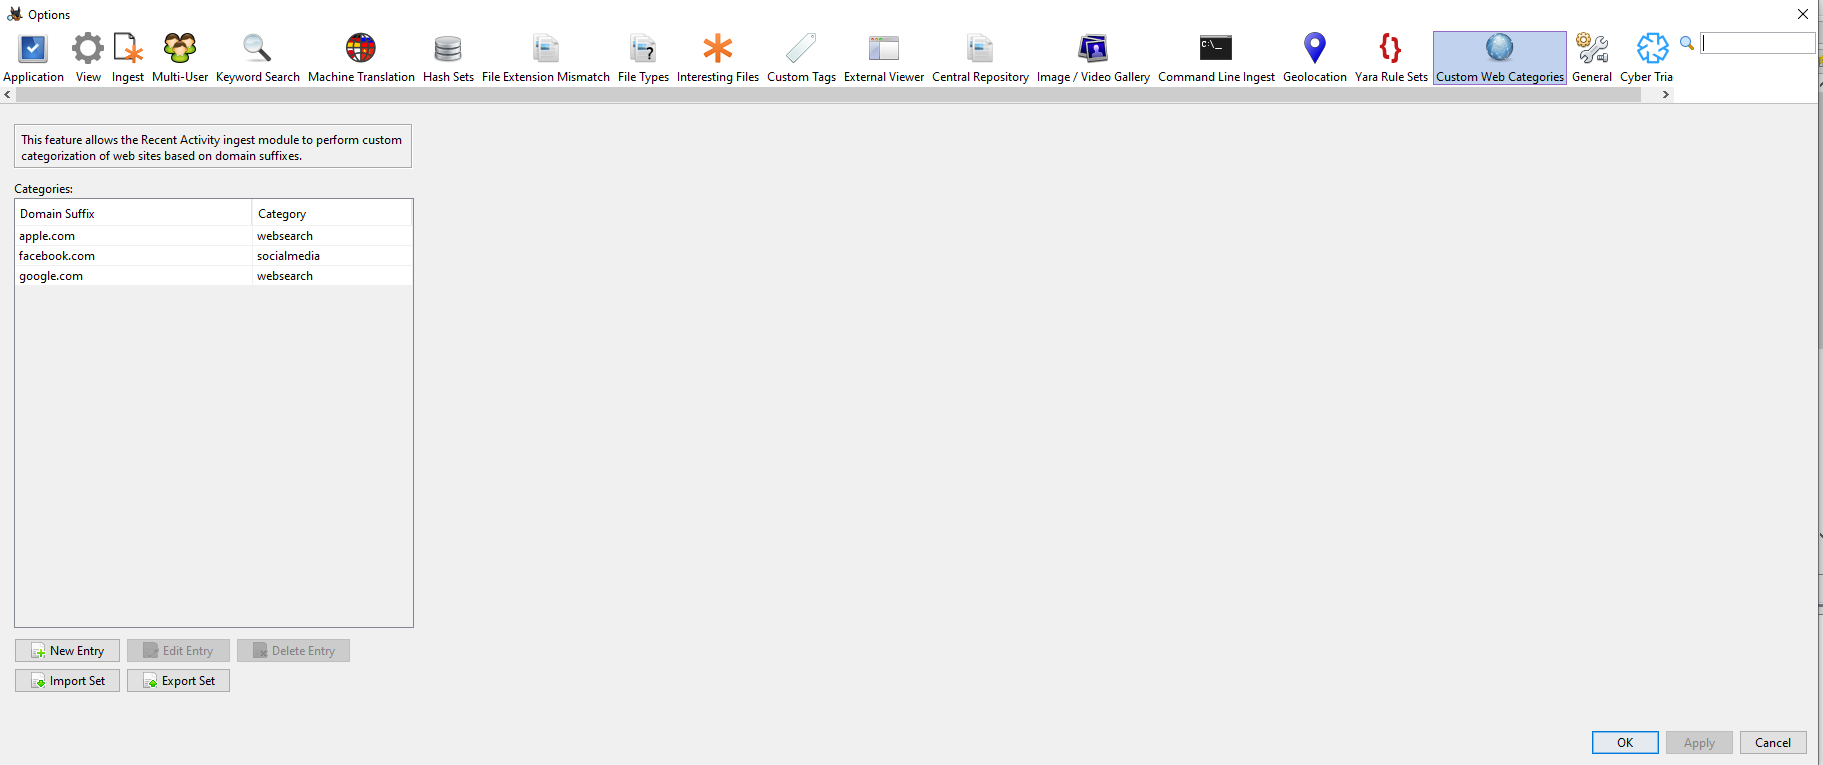
\includegraphics[width=0.75\textwidth]{3/3.1/recent activity settings.PNG}
\end{center}
  \caption{Recent Activity Settings}
\end{minipage}
\hfill
\begin{minipage}{0.45\textwidth}
  \centering
  \begin{center}
    \includegraphics[width=0.75\textwidth]{3/3.1/Screenshot 2024-02-27 at 8.15.21 PM.png}
    \caption{Results of Recent Activity}
\end{center}
\end{minipage}
\end{figure}

\subsubsection*{Results}
The default settings' outcomes are displayed in the \textbf{Data Artifacts} section, while the results of customized settings are shown in the \textbf{Analysis Results } section, one after the other.

\subsection{Hash Lookup}
The Hash Lookup Module computes MD5 hash values for files and cross-references them in a database to classify files as notable, known, or unknown. In Autopsy, the Hash Sets tab enables users to maintain a list of files categorized as known good, meaning they're confirmed safe and can be excluded from routine file checks, saving time and system resources. Additionally, Hash Sets can manage files marked as notable or known bad, helping identify malicious or suspicious content during analysis to enhance security measures. This feature aids in flagging potential security threats or criminal activities for further investigation.

\subsubsection*{Configuring Hash Sets}

To set up custom hash sets in Autopsy, follow these steps:

\begin{enumerate}
  \item Open Autopsy.
  \item Navigate to \textbf{Tools} in the menu bar.
  \item Choose \textbf{Options}.
  \item Access the \textbf{Hash Sets} dialog box.
\end{enumerate}

In the \textbf{Hash Sets} dialog box, you can add known or notable hash sets. Utilize known hash sets such as the NSRL Reference Data Set (RDS) to quickly identify "known" files on a disk image, saving significant time and resources during analysis. Additionally, you have the flexibility to configure known or notable hash sets using your own dataset.

\begin{center}
    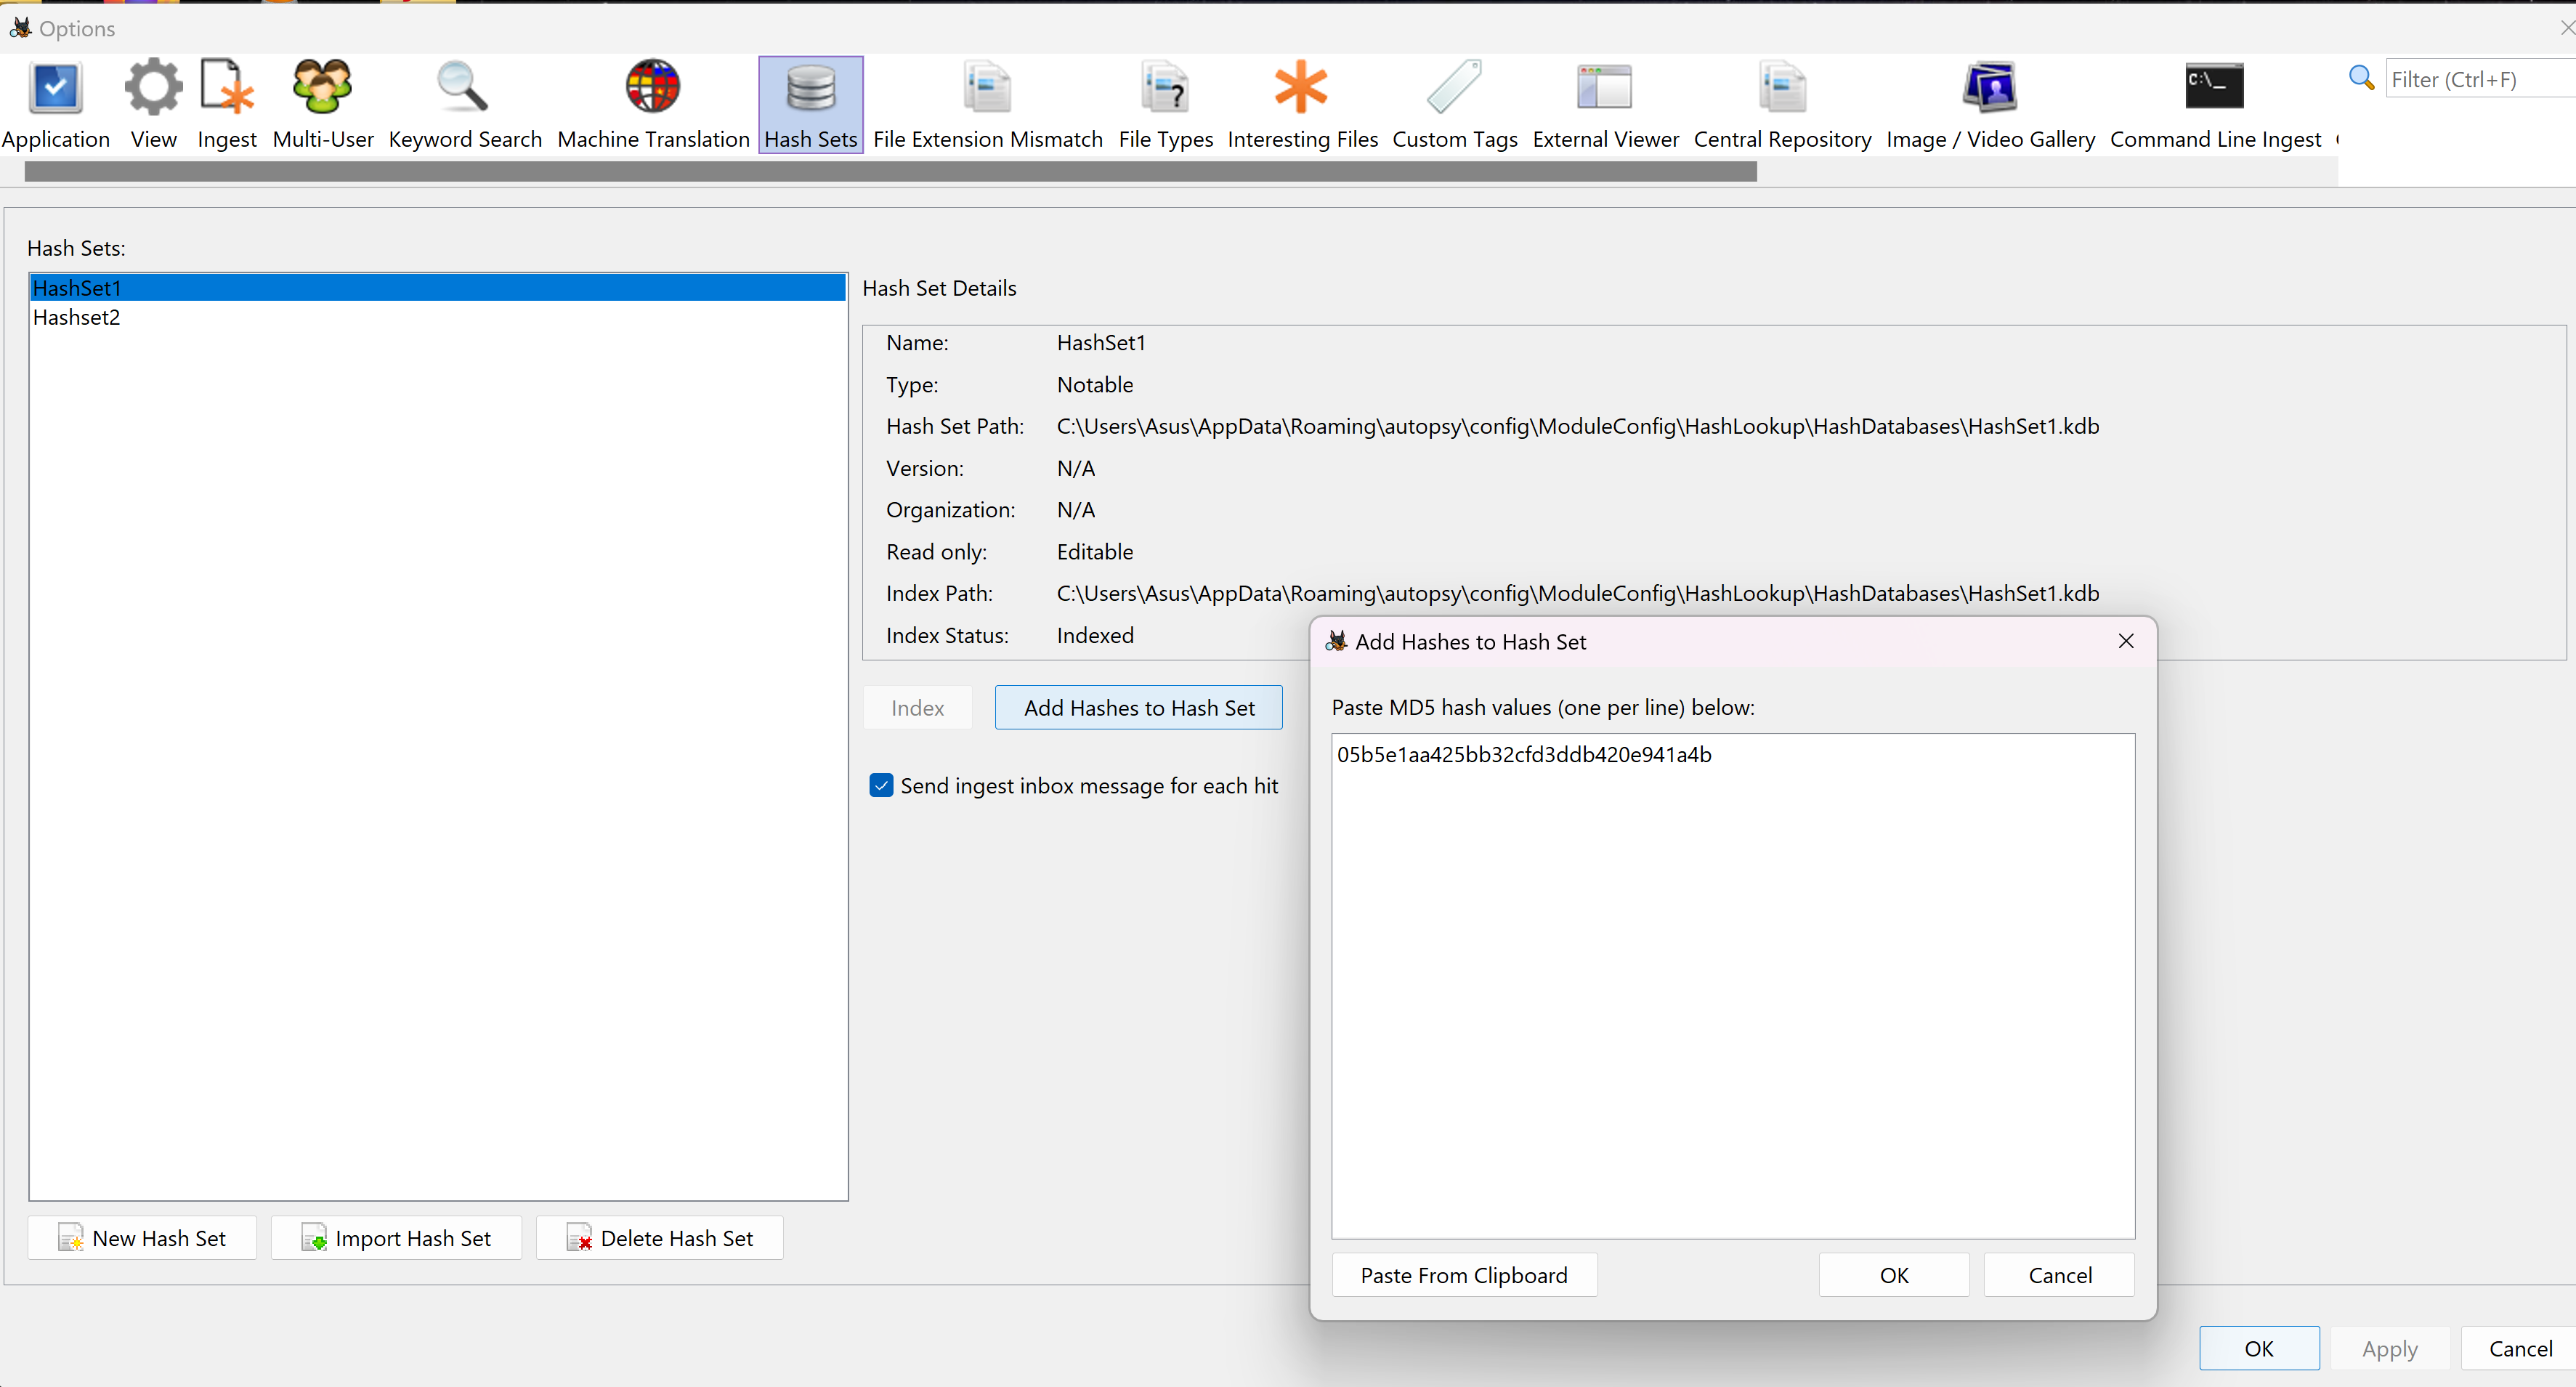
\includegraphics[width=0.75\textwidth]{3/3.2/Hash Set Custom Configuration.png}
\end{center}

\subsubsection*{Results}
In the \textbf{Analysis Results} under \textbf{Hashset Hits}, three matches are identified for files with hash values that correspond to those found in the \textbf{HashSet1} dataset.
\begin{center}
    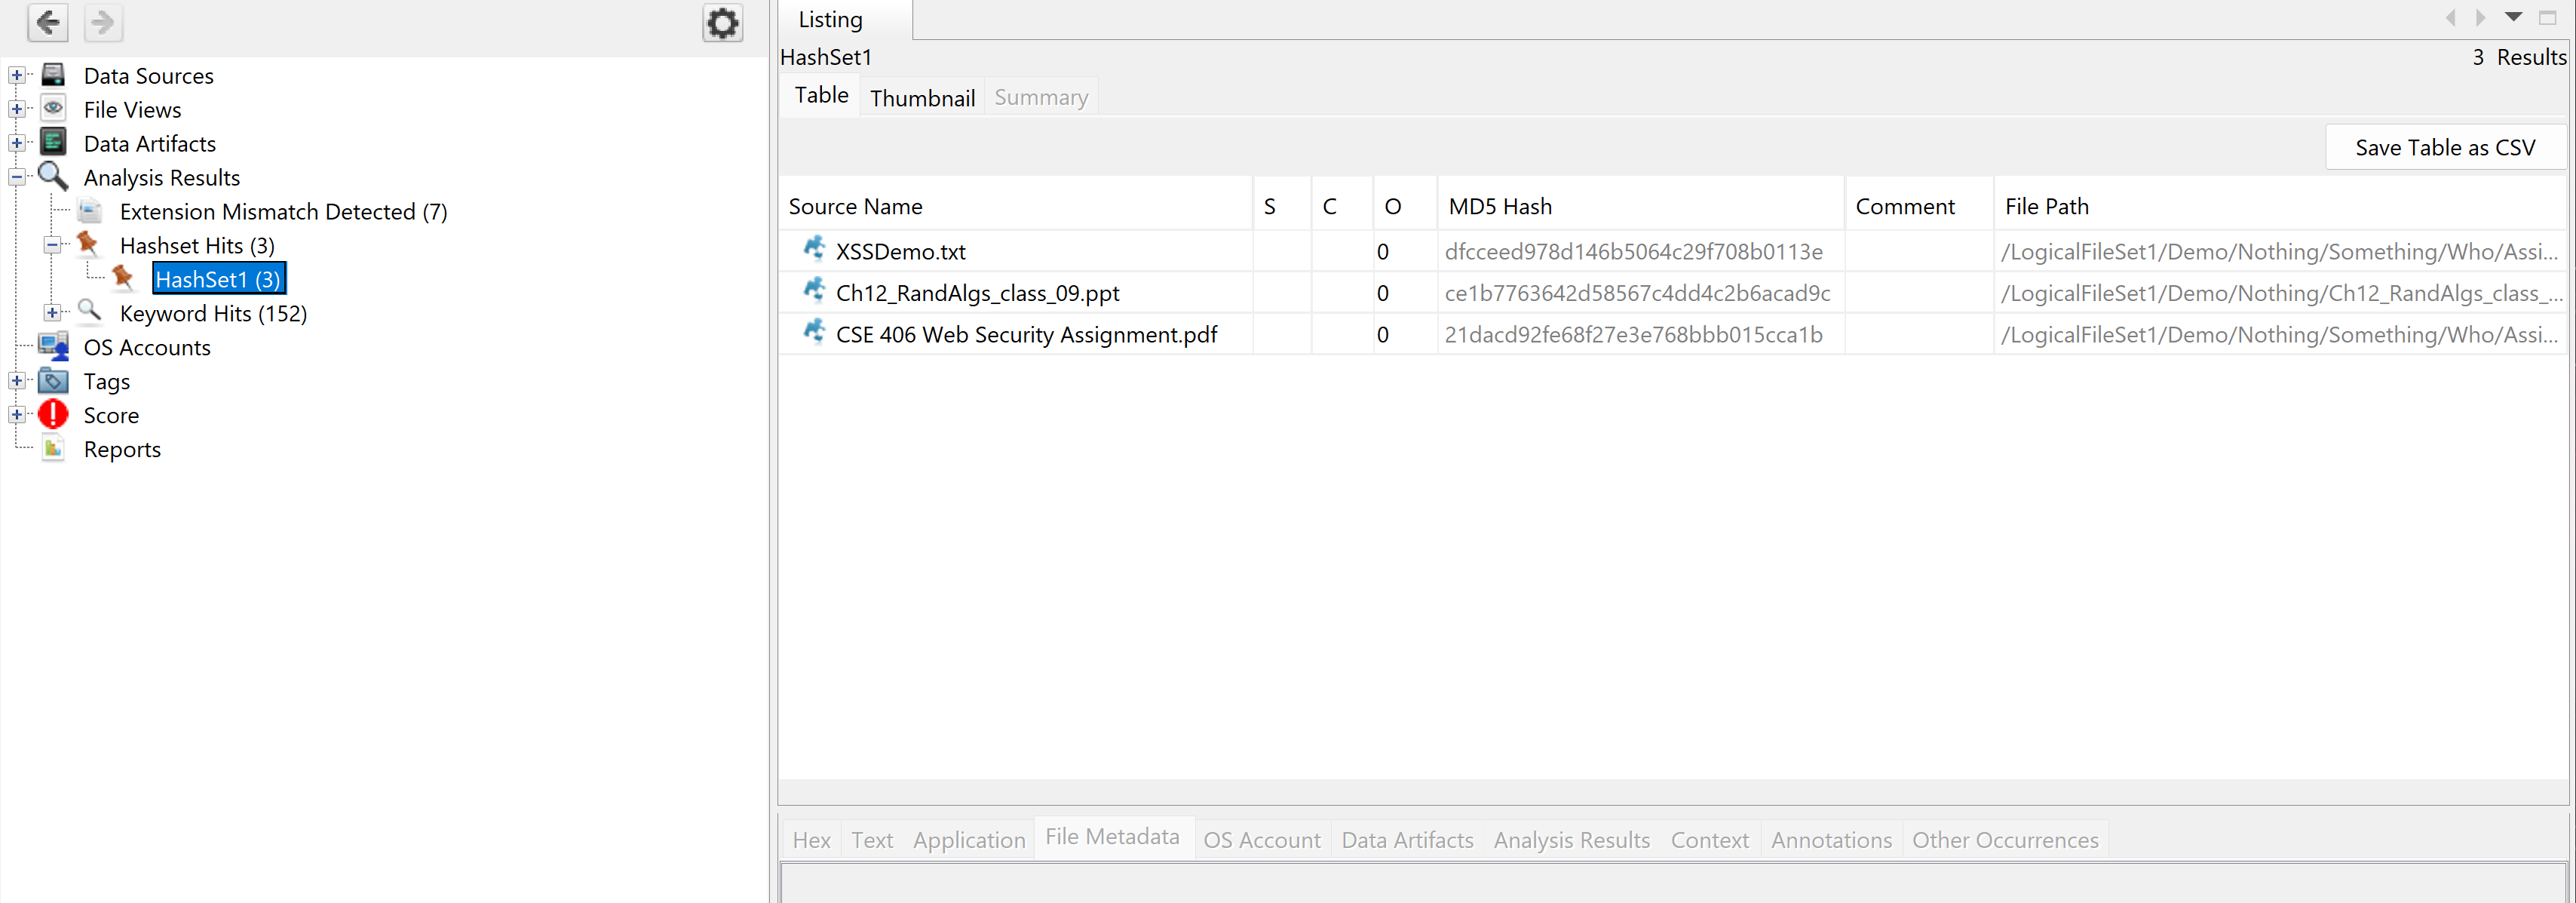
\includegraphics[width=0.75\textwidth]{3/3.2/Results of Hash Lookup ingest module.png}
\end{center}

\subsection{File Type Identification}

Autopsy's File Type ID module is crucial for identifying files based on their inherent signatures, rather than relying solely on file extensions. Utilizing the Tika library, Autopsy can customize criteria to accurately detect primary file IDs. This module plays a pivotal role within Autopsy, enabling the identification of file types within the data source. Moreover, it serves as a foundation for other modules like the \textbf{Extension Mismatch Detector Module} and \textbf{Keyword Search Module}, aiding in comprehensive file type identification within the data set.

\subsubsection*{Configuring Global File Type Identification Settings}
In global file type identification settings, we can configure custom file type of our interst

\begin{center}
    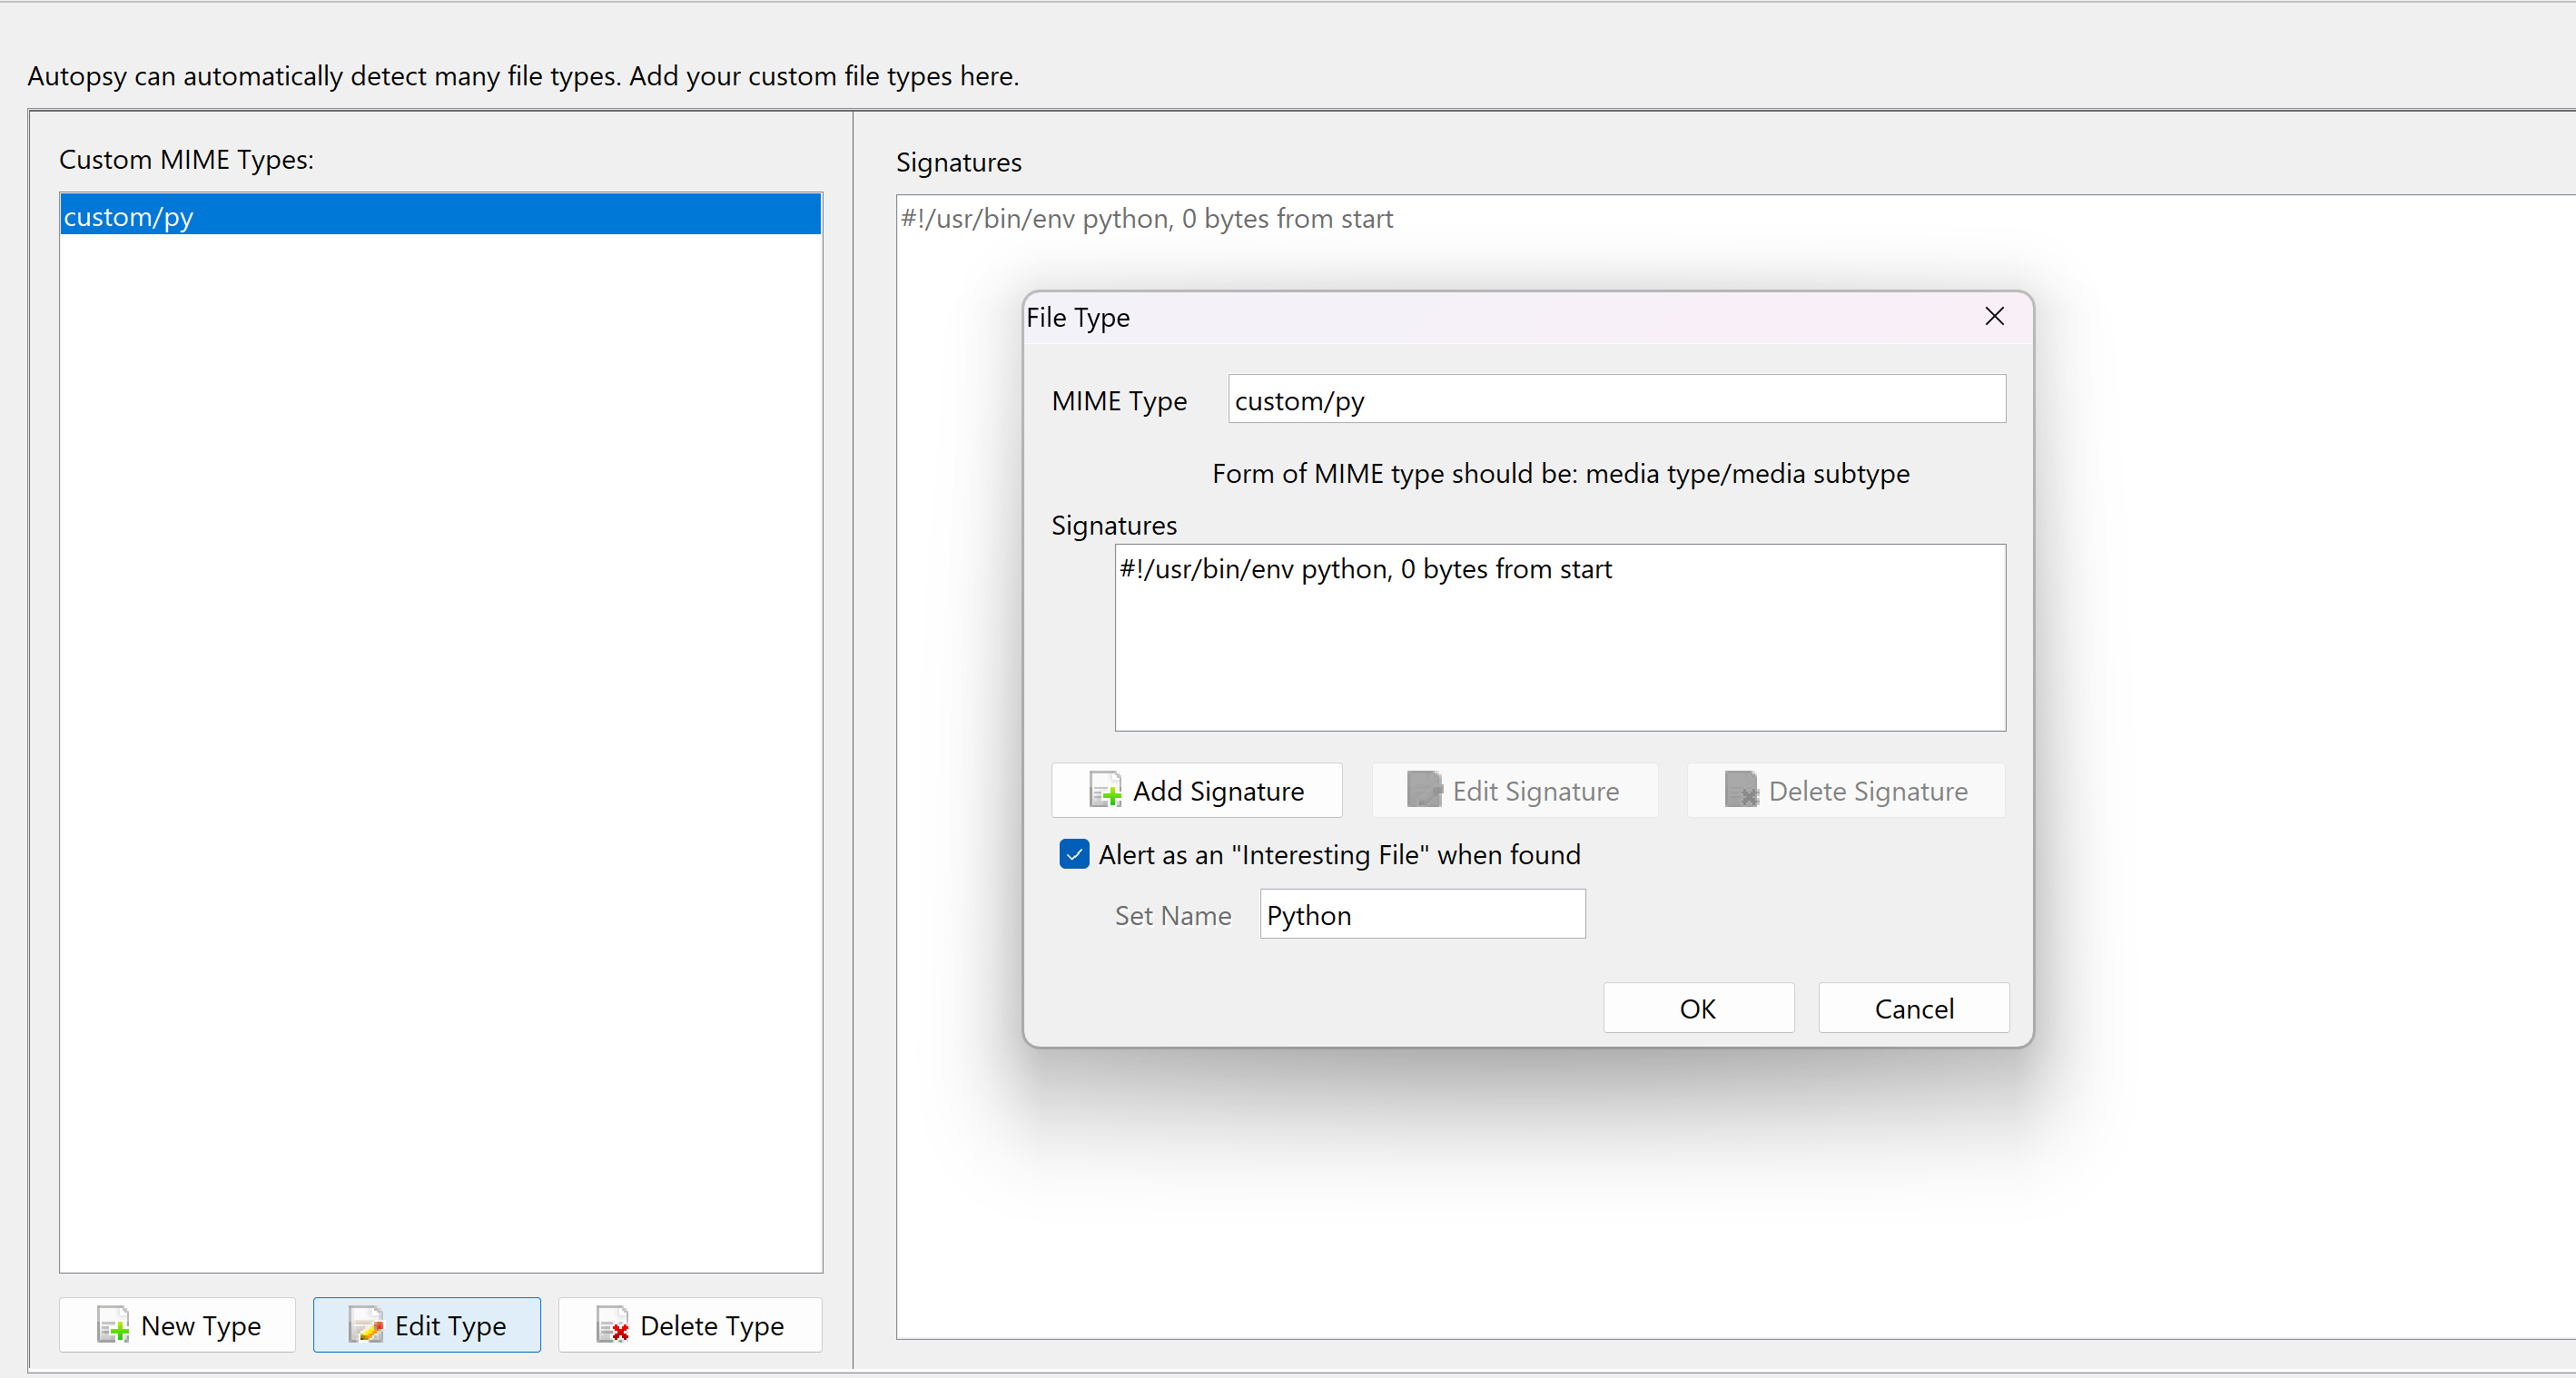
\includegraphics[width=0.75\textwidth]{3/3.3/File Type Identification Settings.png}
\end{center}

\subsubsection*{Results}
In the File Types tab of Autopsy, the results from the \textbf{File Type} Identification module are displayed in two groups: \textbf{By Extension} and \textbf{By Mime Type}. \textbf{By Extension} groups files based on their file extensions, which may sometimes include incorrect files due to corrupted extensions. On the other hand, By Mime Type groups files based on their MIME types. Additionally, results from custom settings are shown grouped according to the specified MIME names in the \textbf{Interesting Items} tab.

\begin{center}
    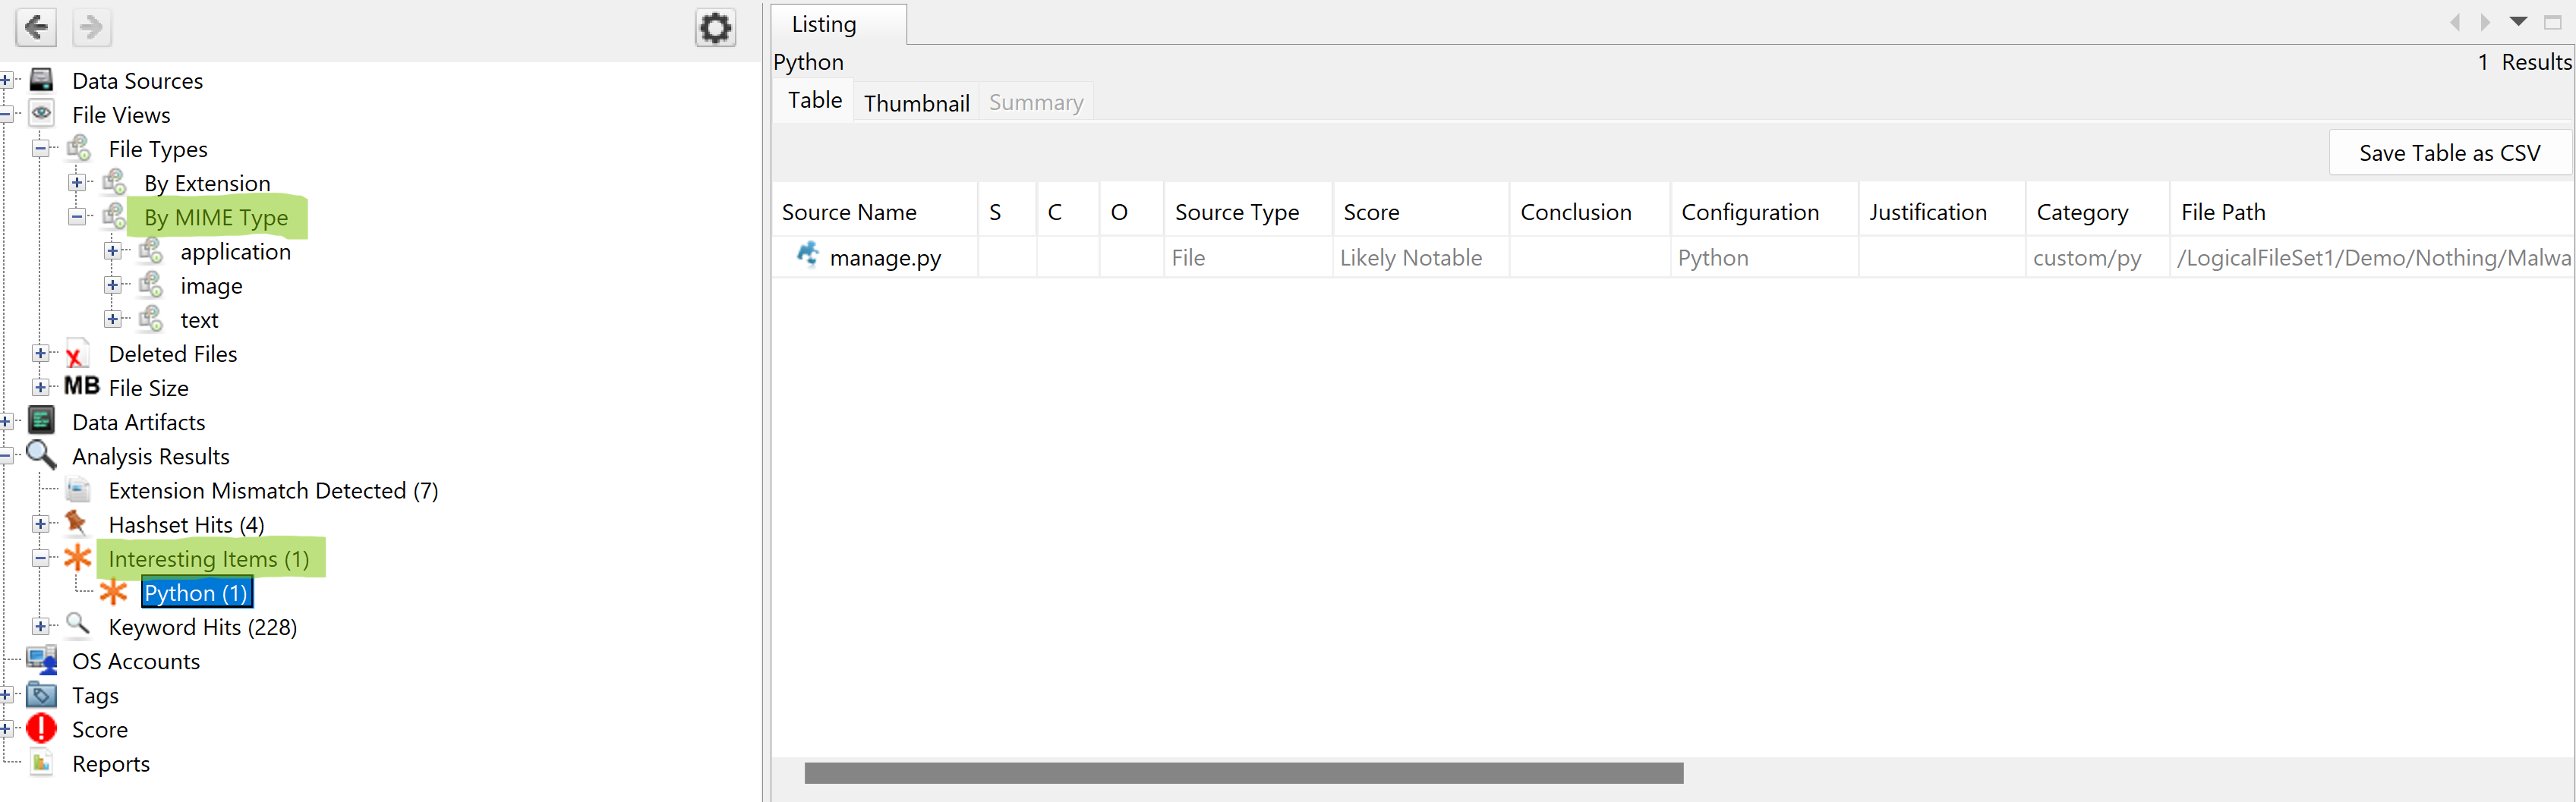
\includegraphics[width=0.75\textwidth]{3/3.3/Custom File Type Identification Settings.png}
\end{center}

\subsection{Embedded File Extractor}
The Embedded File Extractor module in Autopsy can open various archive formats such as ZIP, RAR, and others, as well as document formats like Doc, Docx, PPT, PPTX, XLS, and XLSX. It then sends the extracted files from these formats back through the ingest pipeline for further analysis. This module plays a crucial role in expanding archive files, allowing Autopsy to thoroughly analyze all files within the system. It also enables features like keyword search and hash lookup to examine files contained within these archives. However, it's worth noting that certain media content embedded within document formats like Doc, Docx, PPT, PPTX, XLS, and XLSX may not be extracted by the module.

\subsubsection*{Results}
Each extracted file appears in the data source tree view as a subordinate of the containing archive and as an archive within the \textbf{Views} section under \textbf{File Types } and \textbf{Archives}.

\begin{center}
    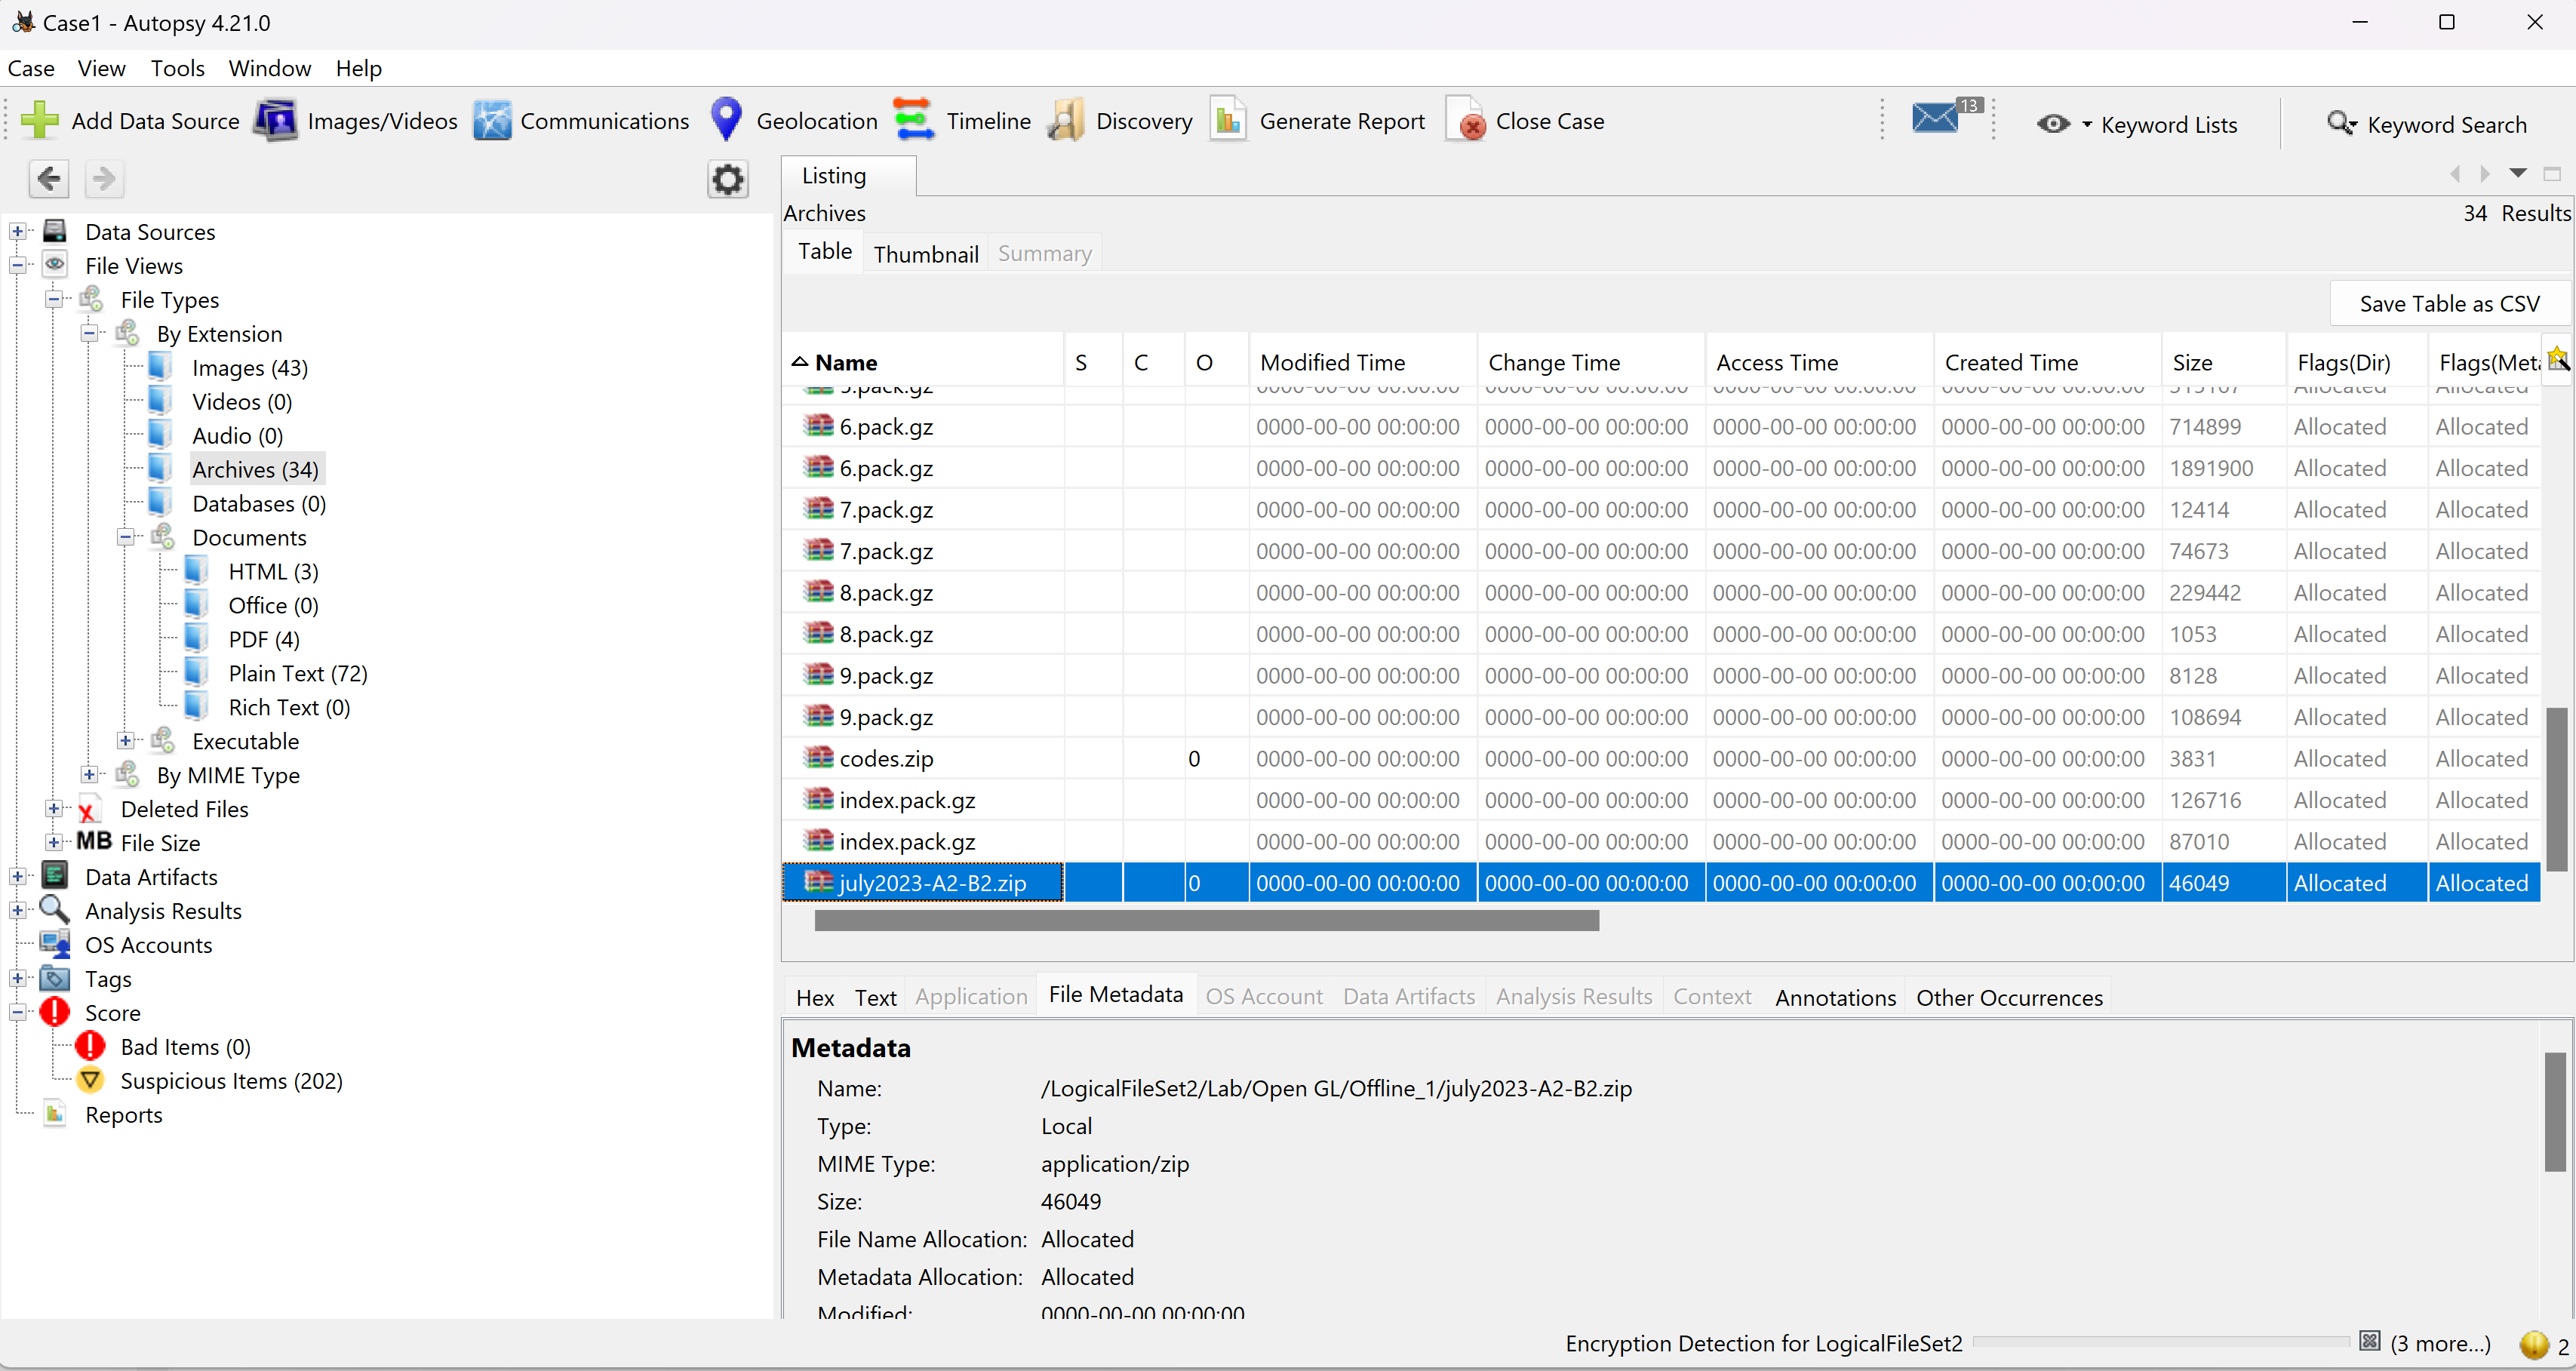
\includegraphics[width=0.75\textwidth]{3/3.4/Embedded File Extractor Results.png}
\end{center}

\subsection{Extension Mismatch Detector}
The Extension Mismatch Detector module utilizes the findings from the File Type Identification module to identify files with extensions that do not typically match their detected file type.

\subsubsection*{Configuring Extension Mismatch Detector Settings}
Within the \lstinline{Tools > Options > File Extension Mismatch} dialog box, users have the capability to both add and remove MIME types along with their corresponding extensions.

\begin{center}
    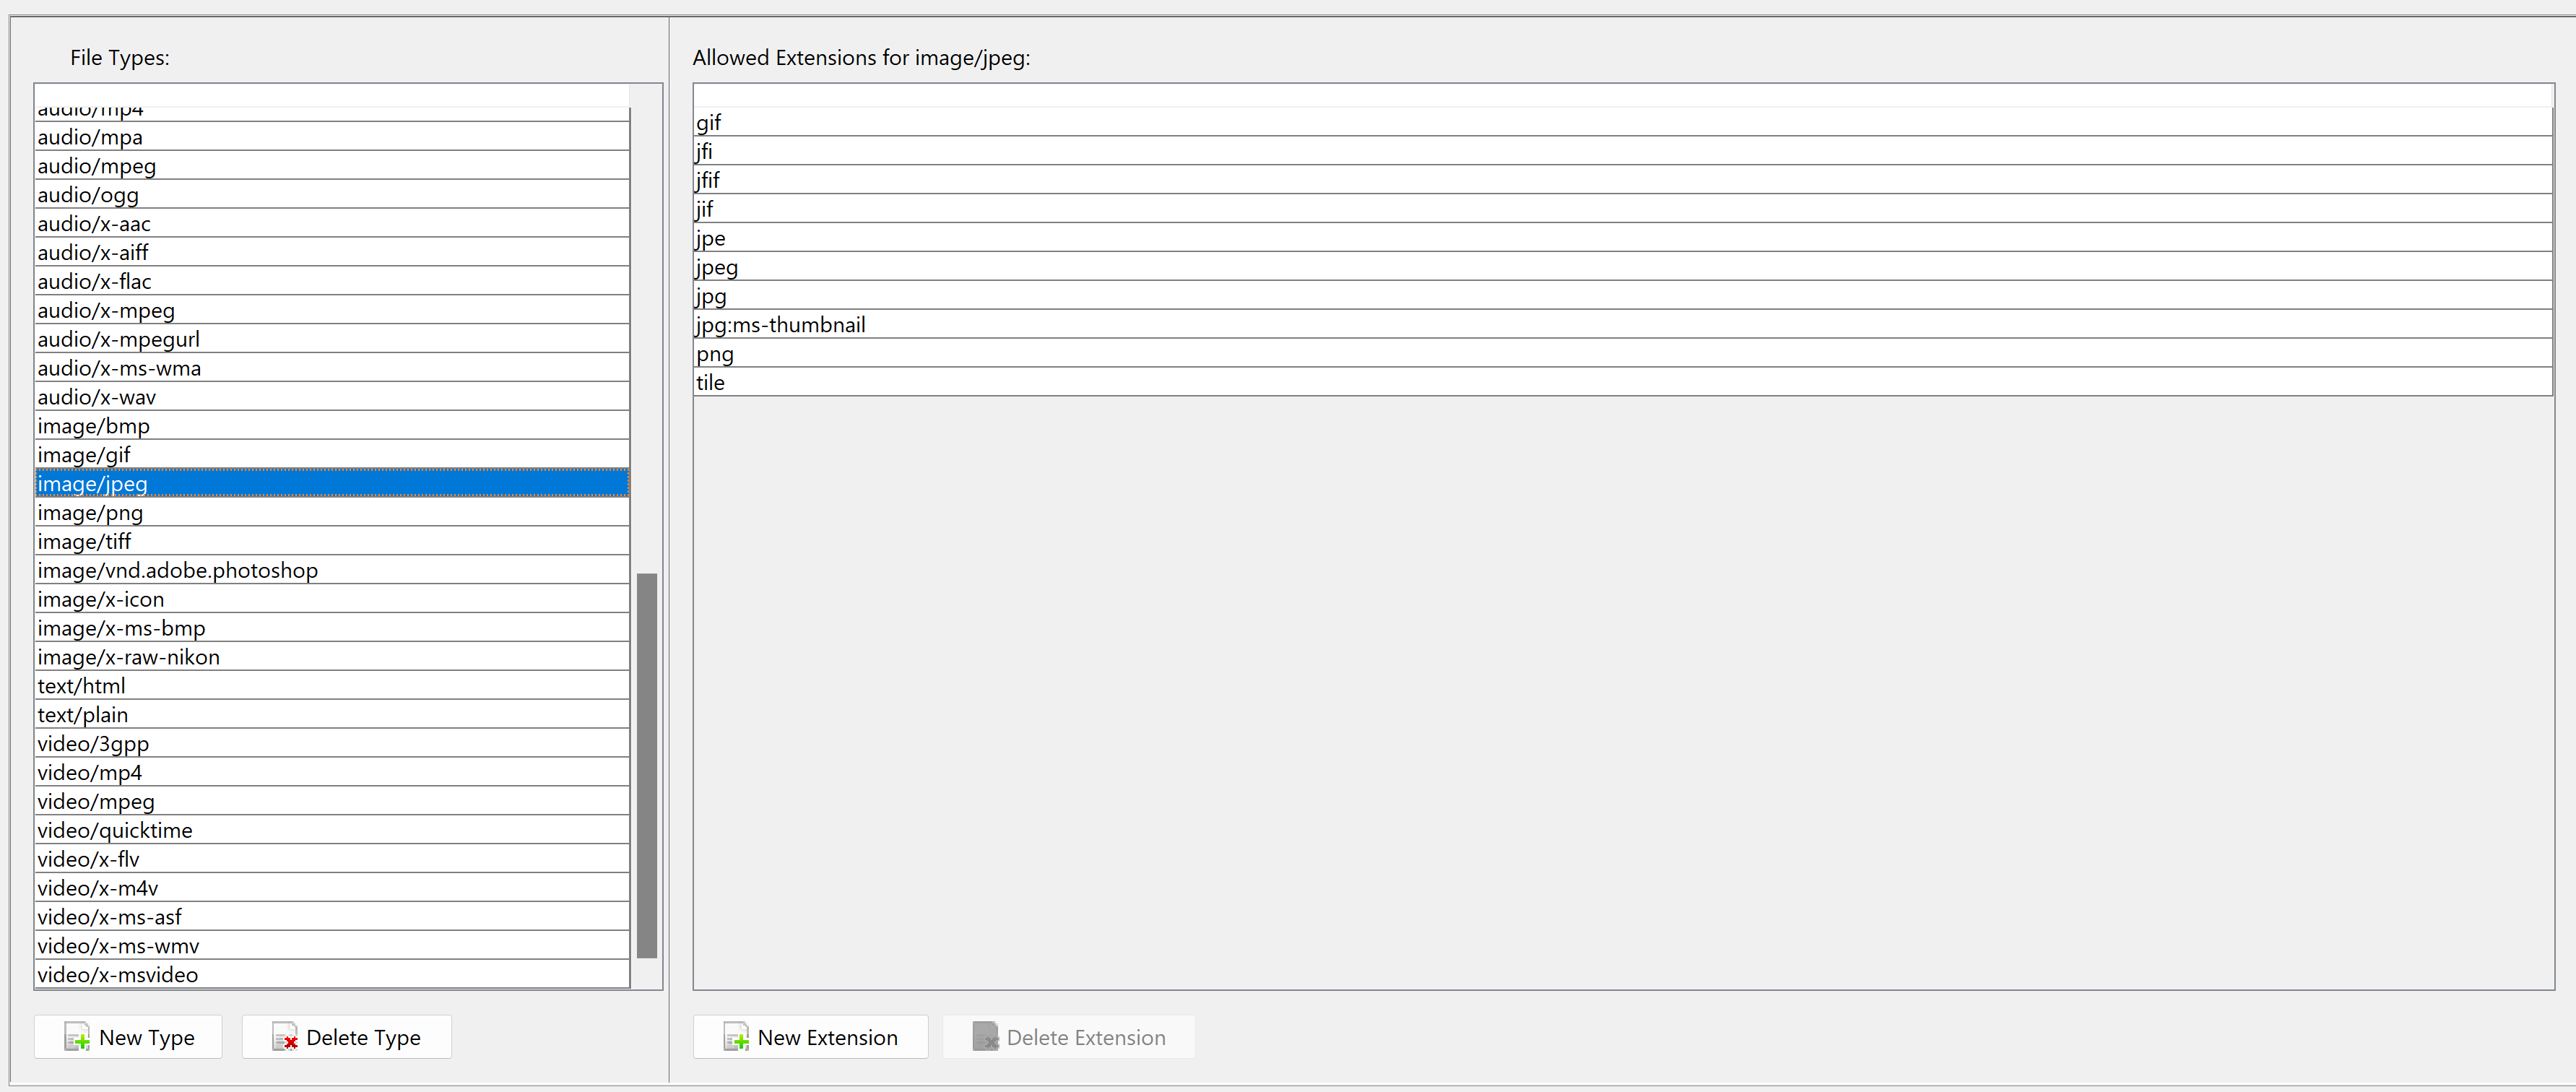
\includegraphics[width=0.75\textwidth]{3/3.5/Extension Mismatch Detector Settings .png}
\end{center}

\subsubsection*{Results}
Results are shown in \texttt{Analysis Results > Extension Mismatch Detected}.

\begin{center}
    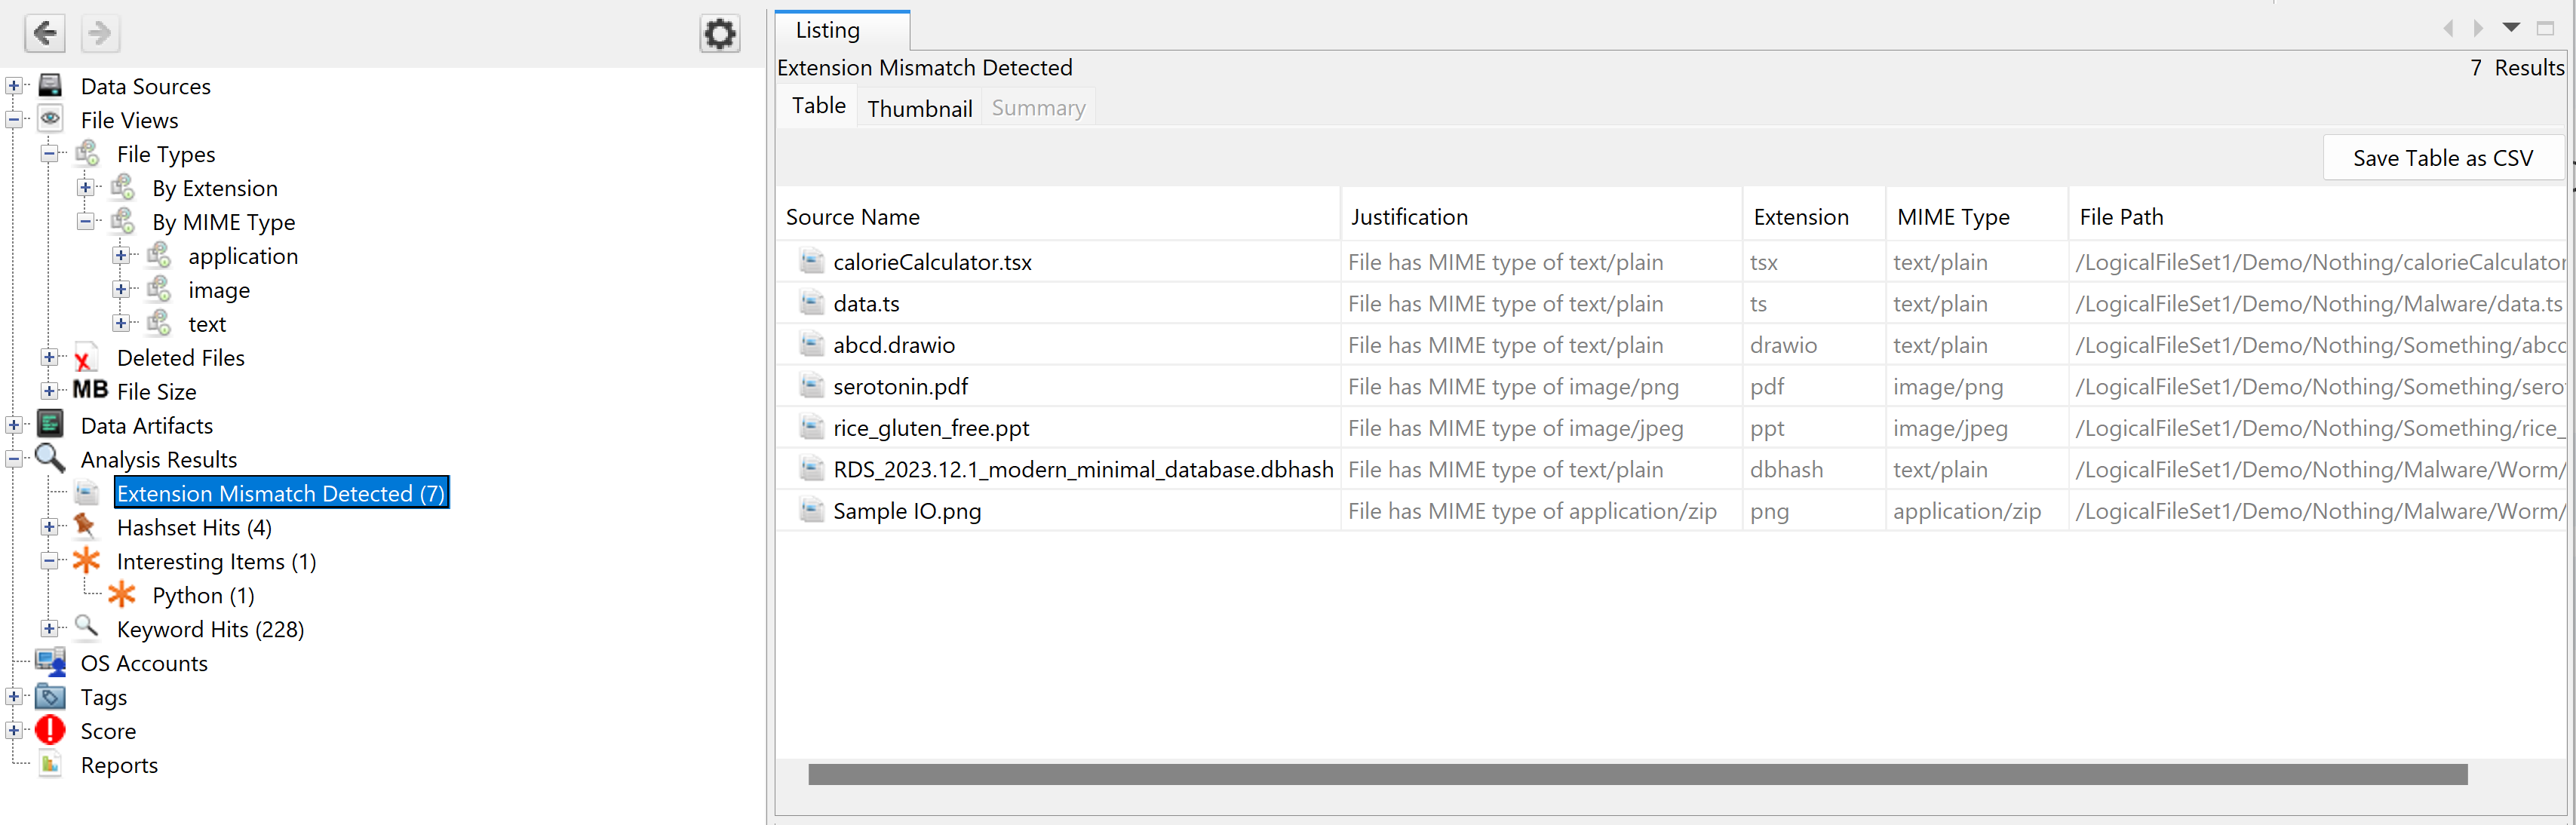
\includegraphics[width=0.75\textwidth]{3/3.5/Details of Mismatched Files.png}
\end{center}

\subsection{Picture Analyzer}
The Picture Analyzer module in Autopsy retrieves important information from images, such as location, date, time, camera model, and settings, known as EXIF metadata. This data is then added to the Blackboard for further analysis, providing insights into the photograph's details like where and when it was taken, and what camera was used. Additionally, the module converts HEIC/HEIF photos to JPG format while keeping their EXIF data intact, ensuring they are treated and saved just like regular JPG images.

\subsubsection*{Results}
The outcomes are displayed in the result trees.
\begin{center}
    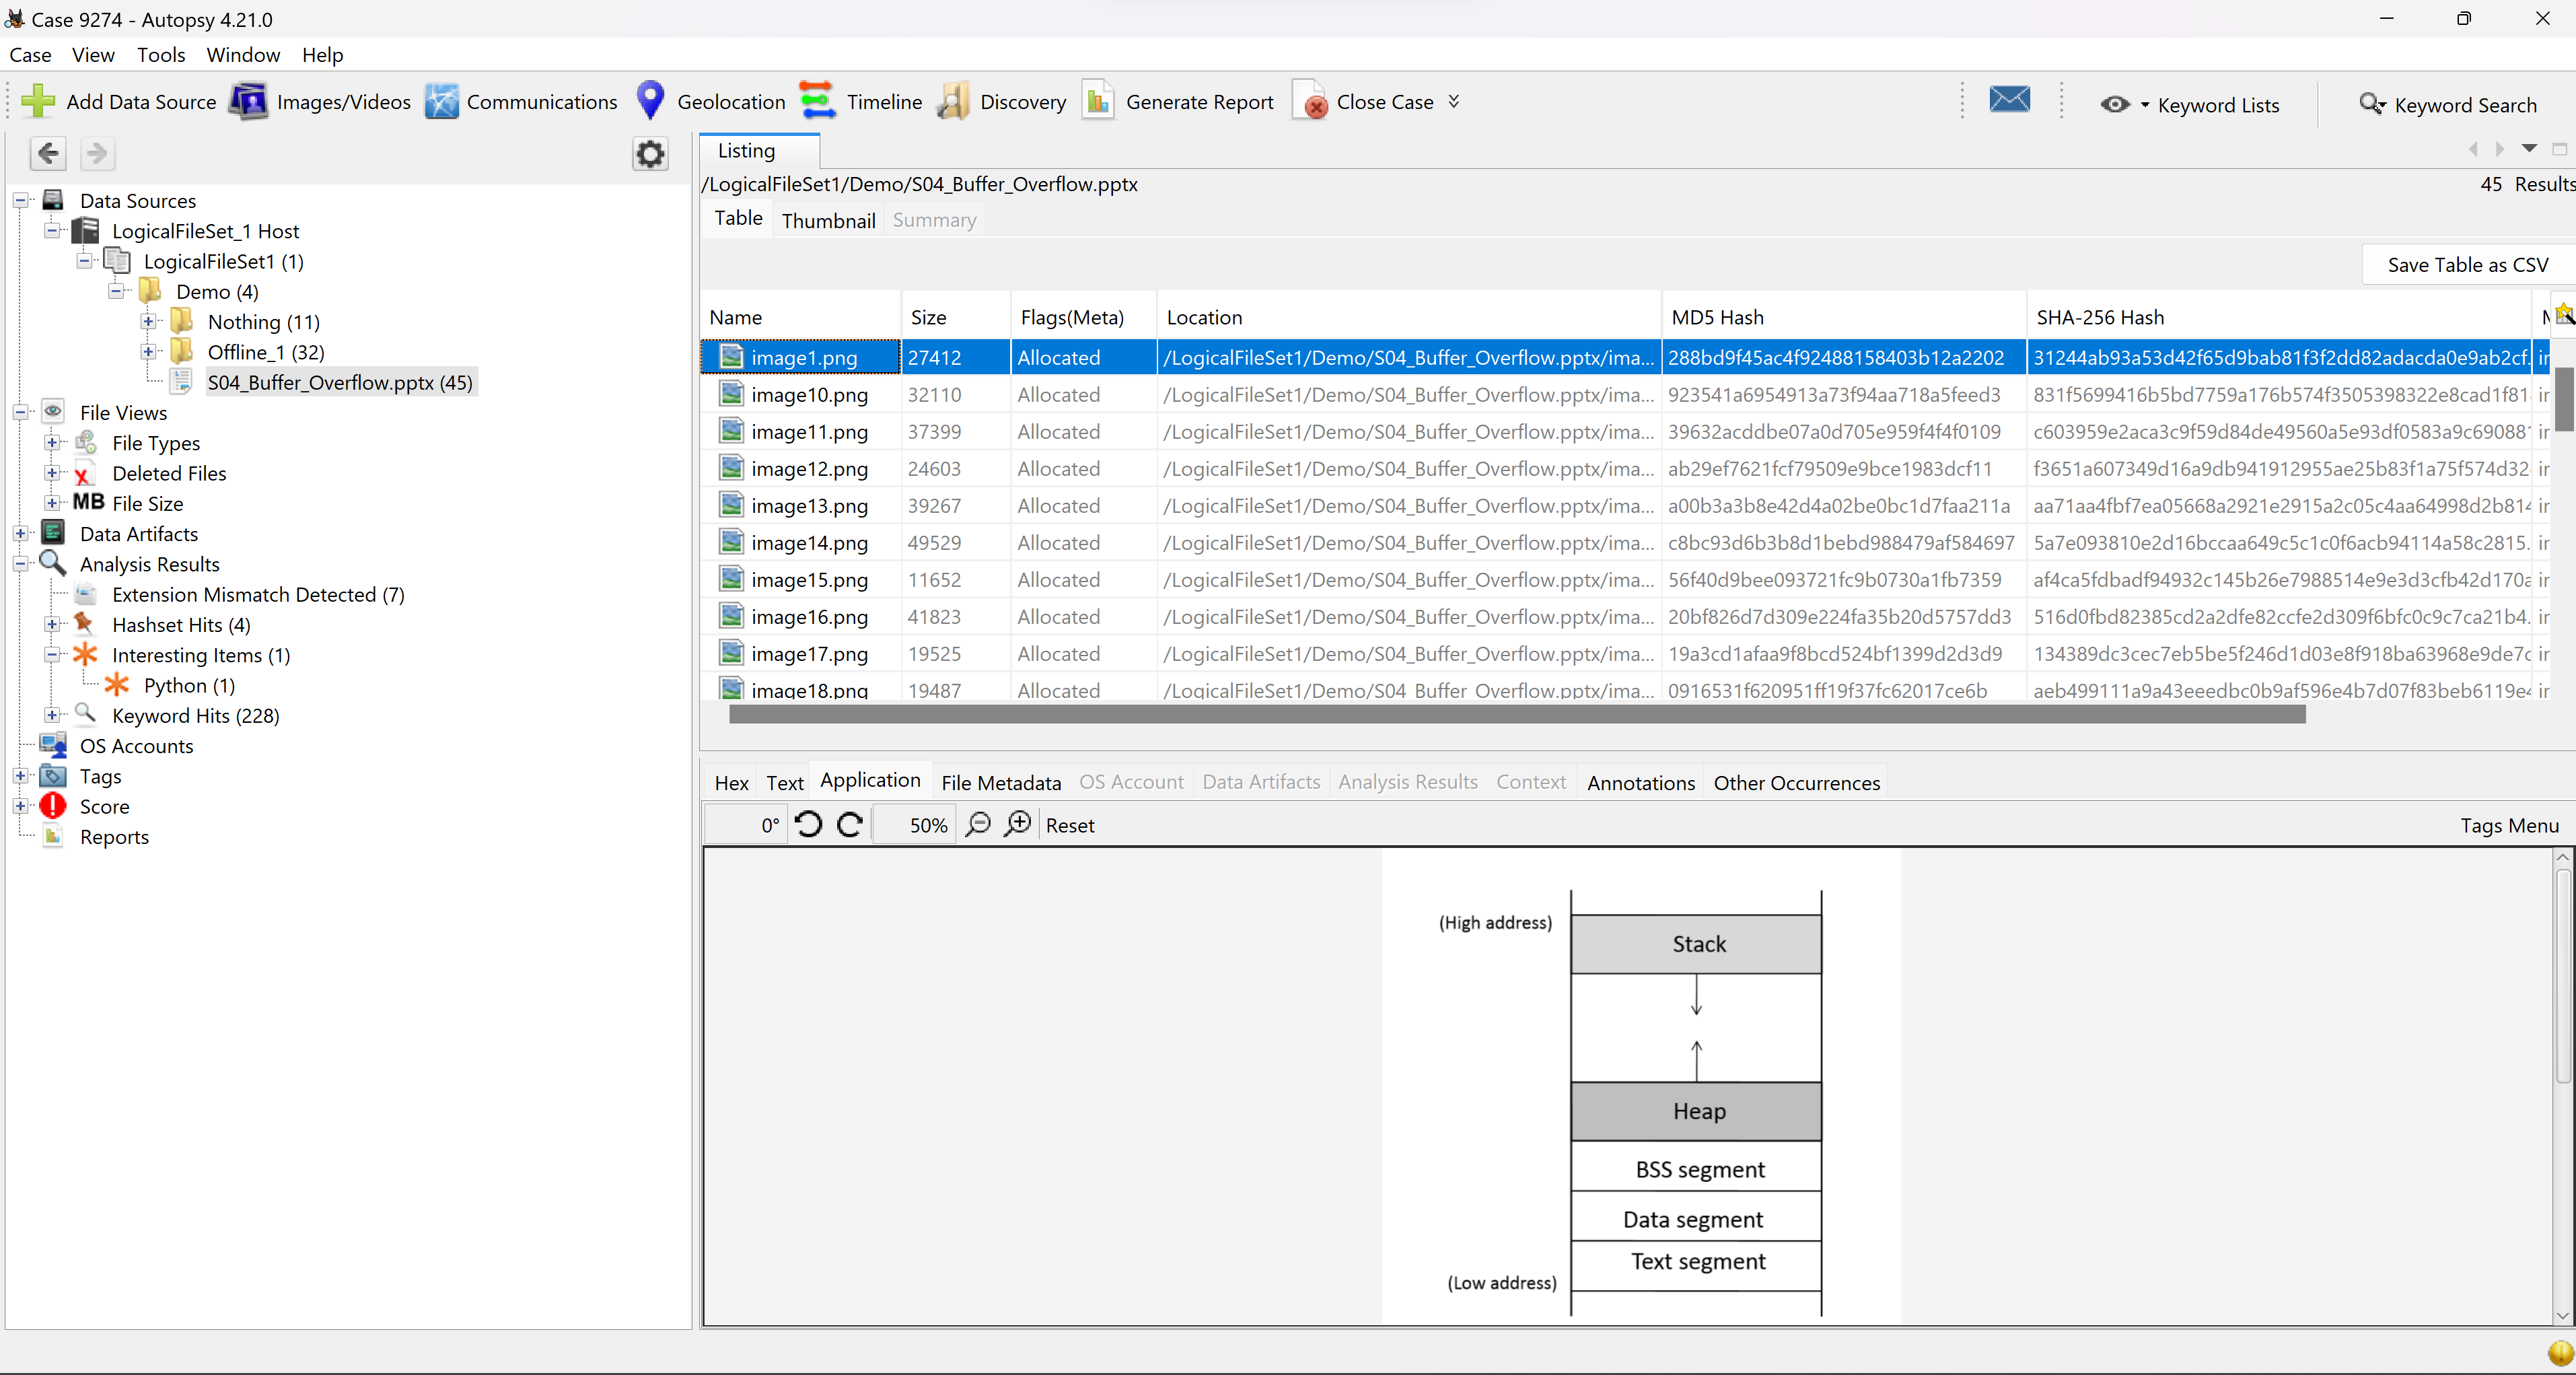
\includegraphics[width=0.75\textwidth]{3/3.6/Picture Analyzer Results.png}
\end{center}

\subsection{Keyword Search}
The Keyword Search module enables searching during the ingest process and also supports manual text searches post-ingest (refer to Ad Hoc Keyword Search). It extracts text from ingested files, selected reports generated by other modules, and results from other modules. Users can specify keywords to search for, add regular expressions for searching, and include keywords to exclude from the search.

\begin{center}
    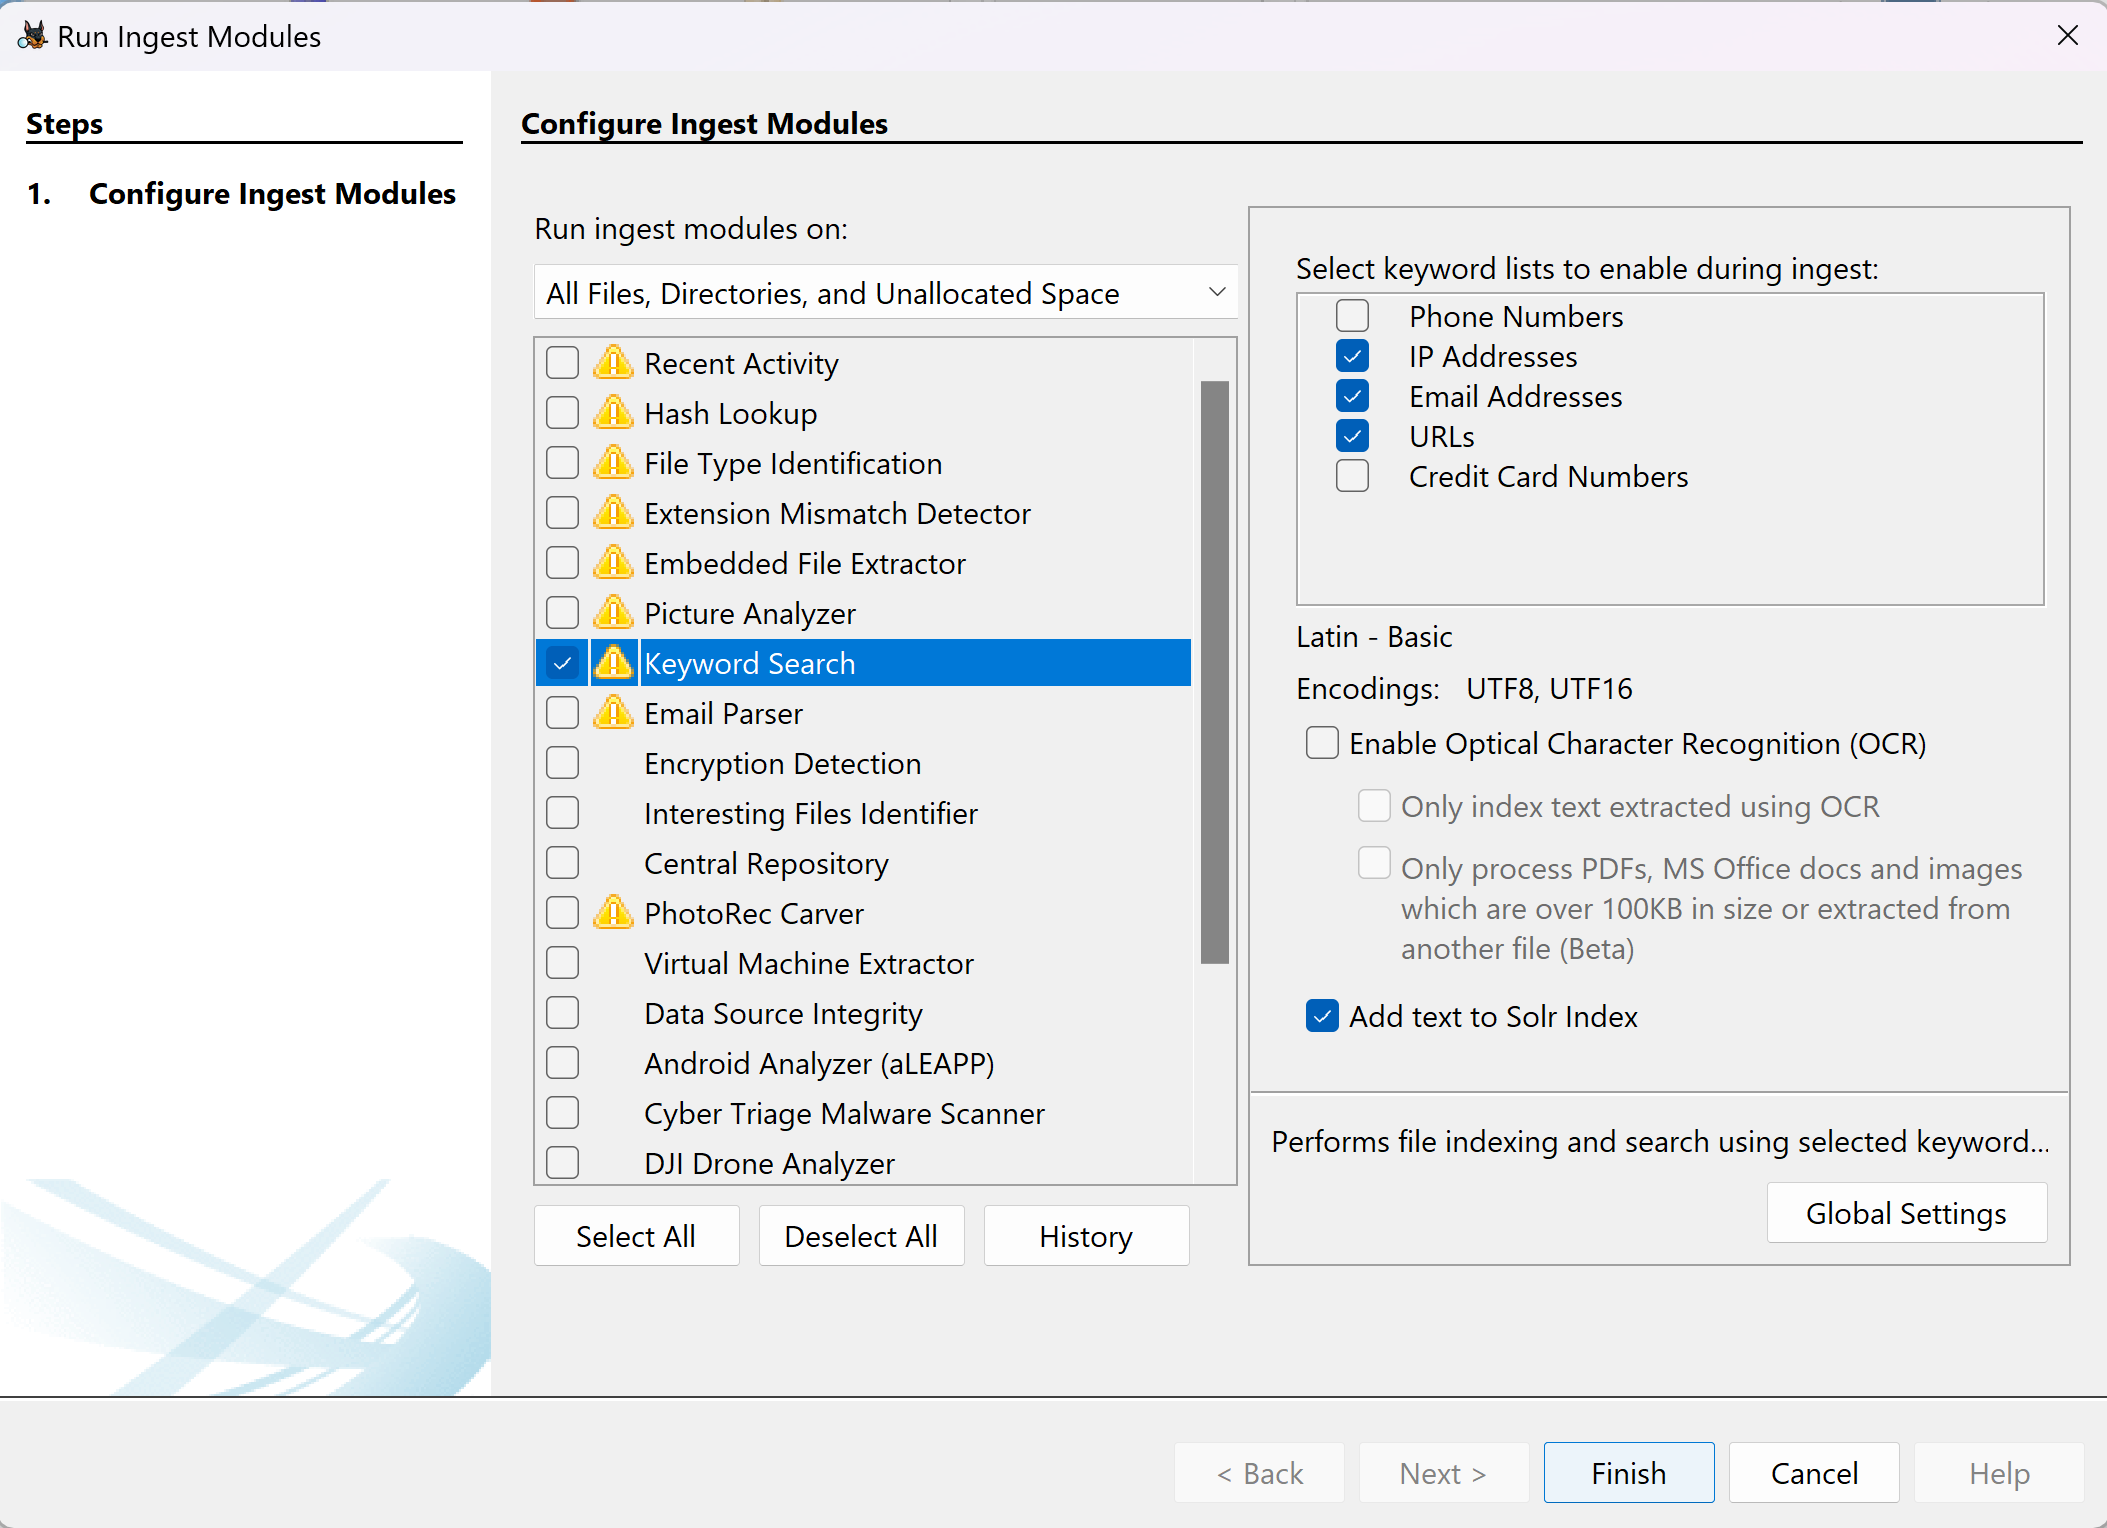
\includegraphics[width=0.75\textwidth]{3/3.7/Keyword Search Settings.png}
\end{center}

\subsubsection*{Results}
In the global settings options, users can incorporate custom keyword rules for searching. When this module is executed, it searches for specified keywords within files and their metadata. The search results are displayed in \texttt{Analysis Results > Keyword Hits}, grouped together by the detected keyword.

\begin{center}
    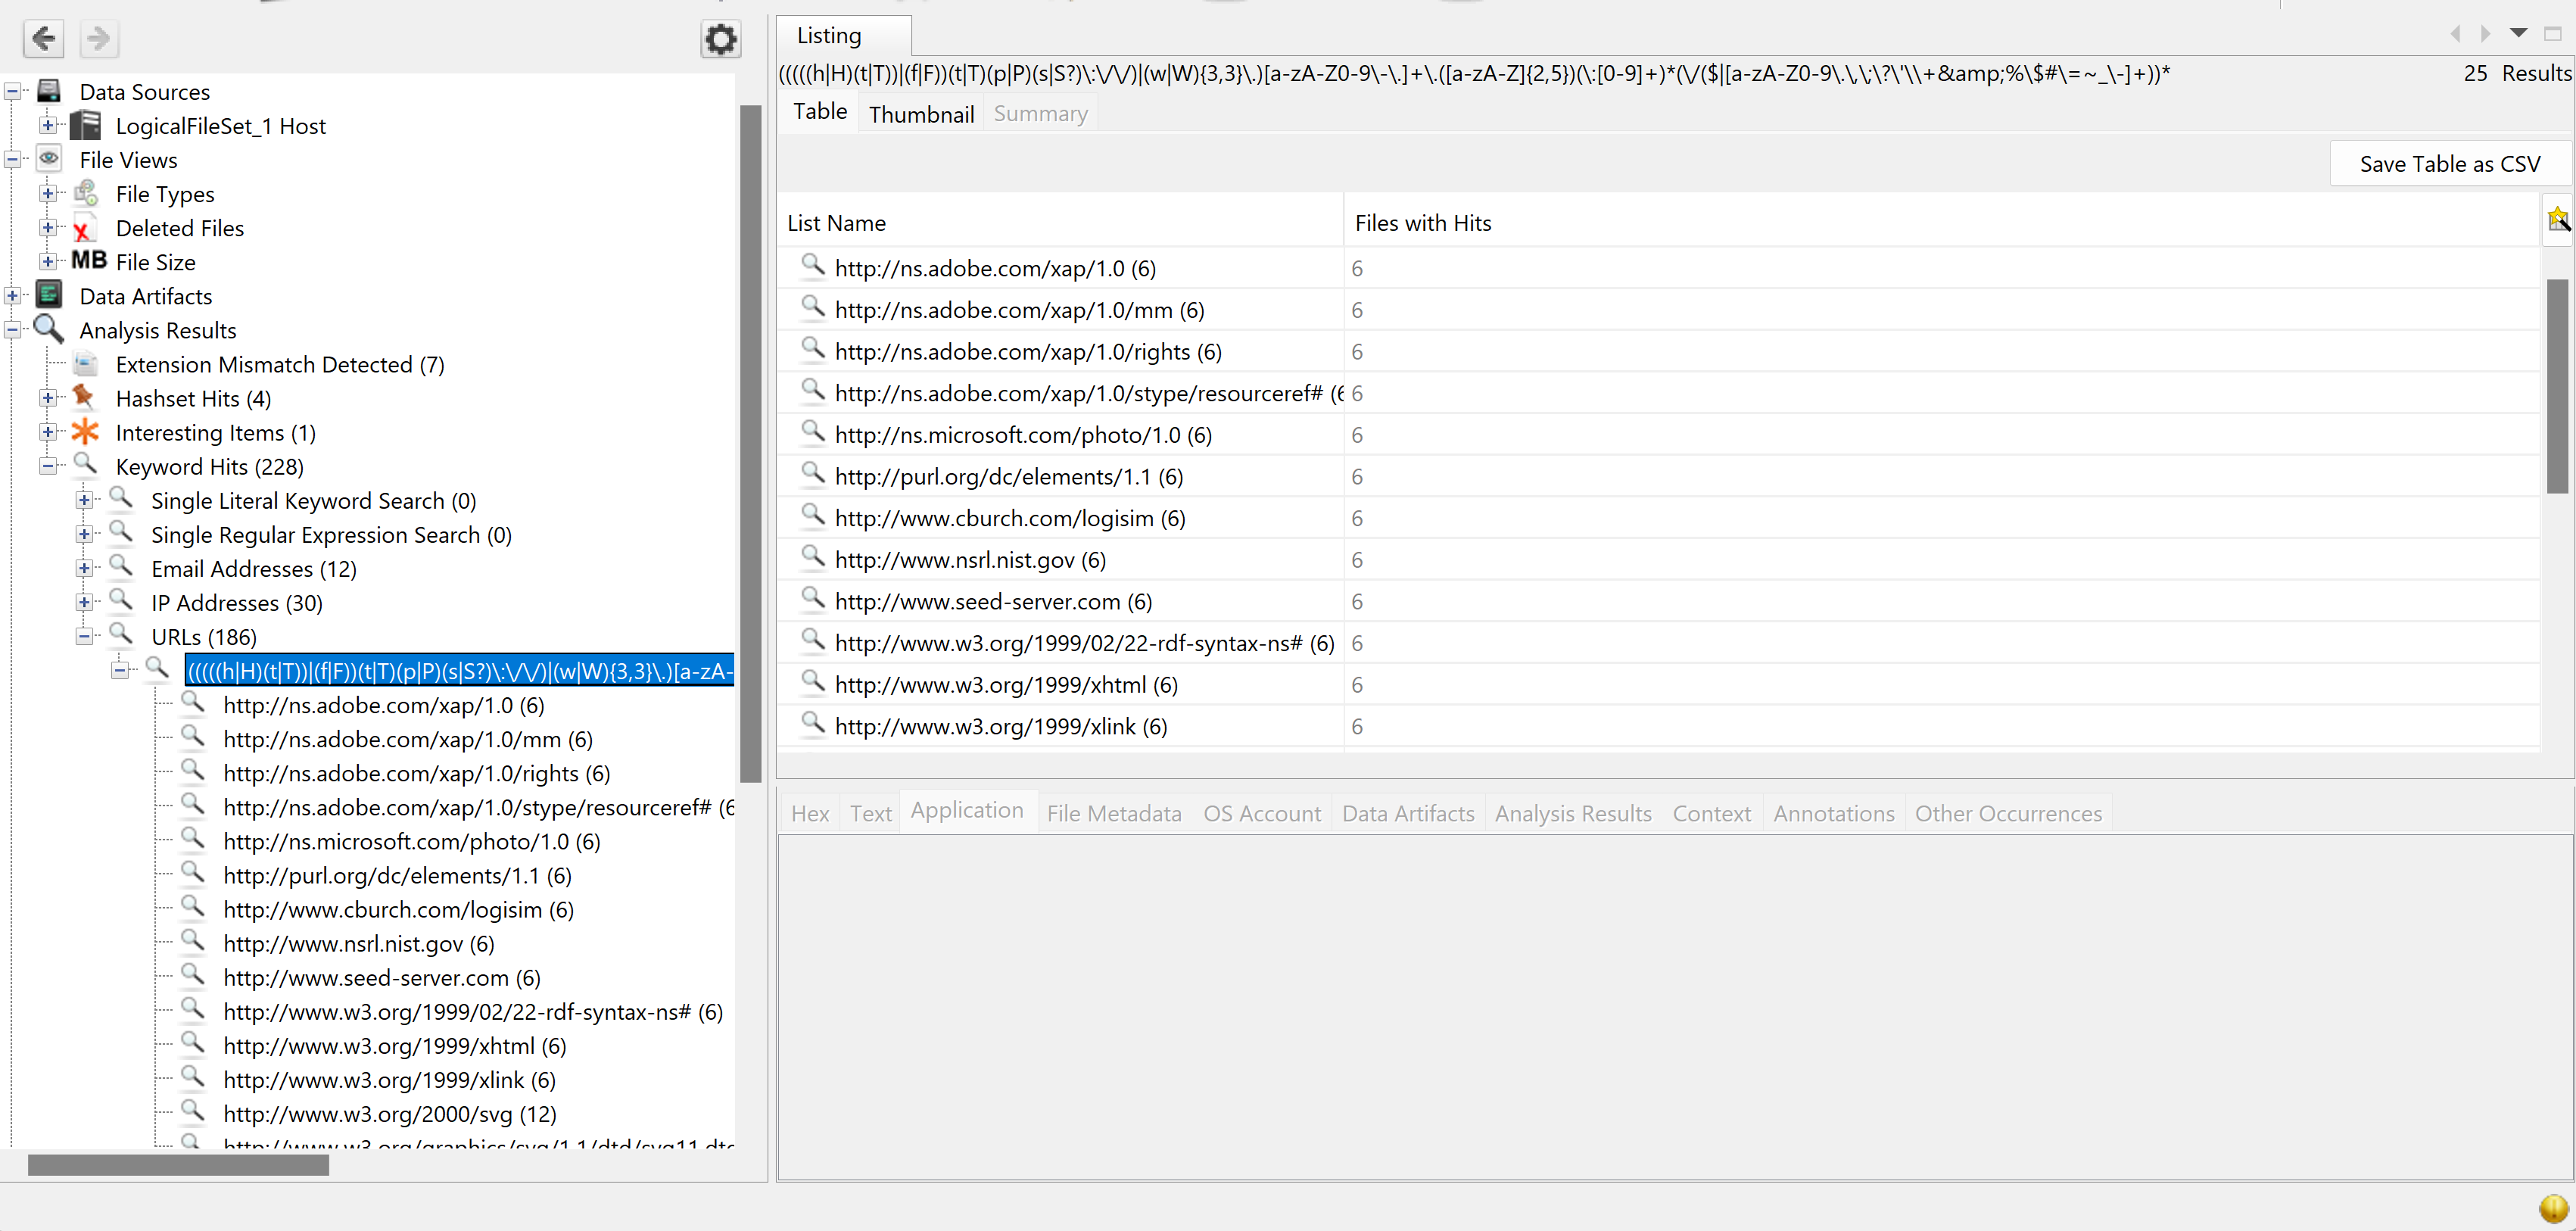
\includegraphics[width=0.75\textwidth]{3/3.7/Keyword Search Results Details.png}
\end{center}

\subsection{Interesting Files Identifier}
The Interesting Files Identifier module automatically flags files and directories that adhere to predefined criteria. This feature proves beneficial for verifying the presence of files with specific names or paths within the data source, or when files of particular types consistently warrant attention.

\subsubsection*{Configuring Interesting Files Settings}
\begin{itemize}
    \item Users can define a set of rules by accessing the \texttt{Tools > Options > Interesting Files} dialog box.
    \item For instance, in our demonstration, we established a rule set named "Suspicious."
    \item Within this set, we incorporated two specific rules:
    \begin{enumerate}
        \item If any file contains the substring "Worm" in its name, it will be categorized as an "interesting file."
        \item Similarly, if any file contains the substring "virus" in its name, it will also be categorized as an "interesting file."
    \end{enumerate}
\end{itemize}

\begin{center}
    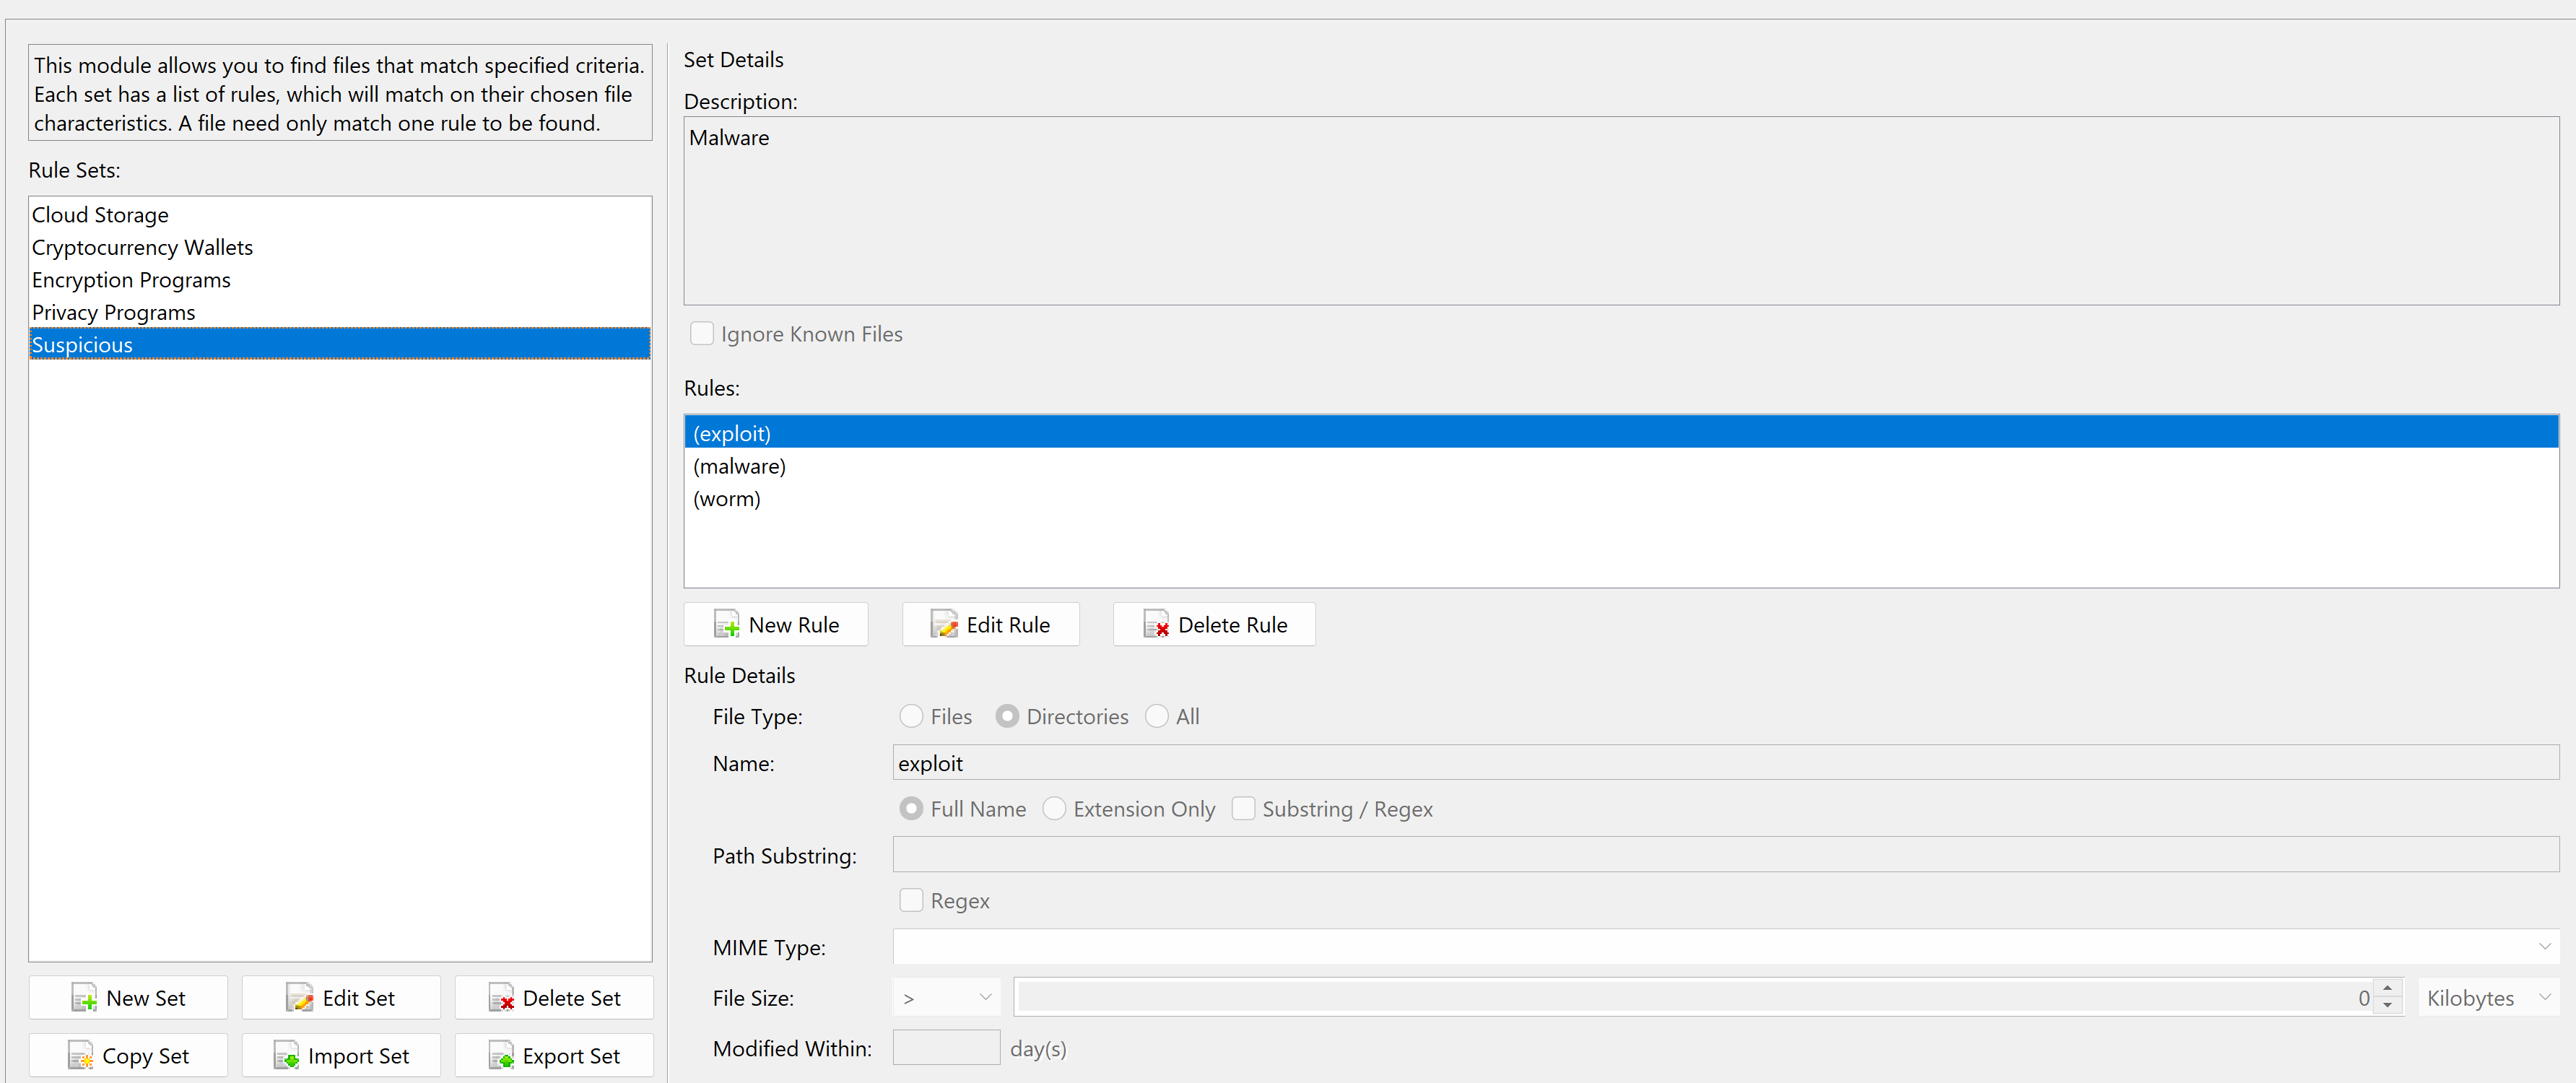
\includegraphics[width=0.75\textwidth]{3/3.8/Interesting Files Configuration.png}
\end{center}

\subsubsection*{Results}
After running the "Interesting Files Identifier" ingest module, the results can be viewed in \texttt{Analysis Results > Interesting Items}. Three files have been identified as interesting items due to their names containing the substrings "worm" or "virus," as defined within the "Suspicious" set of rules.

\subsection{Email Parser}
The Email Parser module recognizes MBOX, EML, and PST format files by their signatures. It extracts emails from these files and adds the results to the Blackboard. Additionally, it identifies the email accounts used in the discovered emails.

\subsubsection*{Results}

\begin{center}
    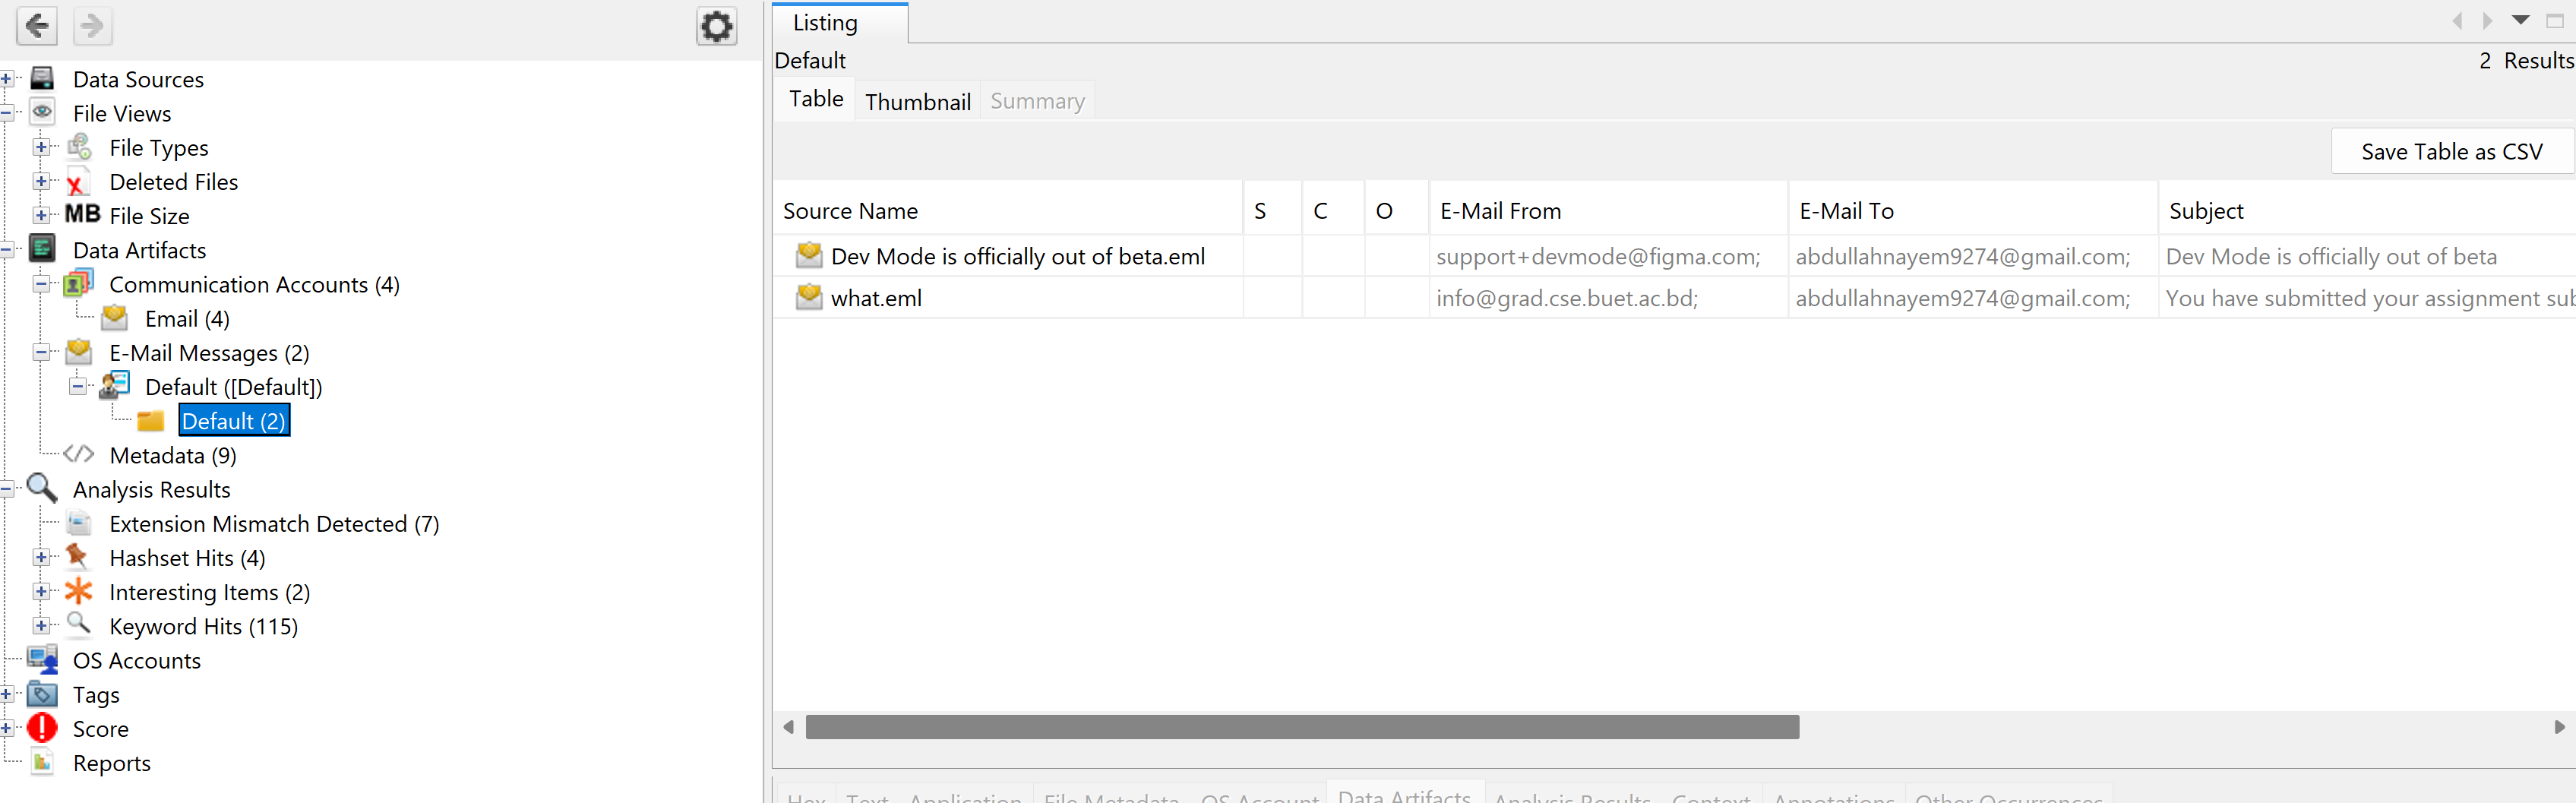
\includegraphics[width=0.75\textwidth]{3/3.9/Results of Email Parser ingest module.png}
\end{center}

After running the "Email Parser" ingest module, the results can be viewed in \texttt{Data Artifacts > E-mail messages}. Two email files have been identified by the module.

\begin{center}
    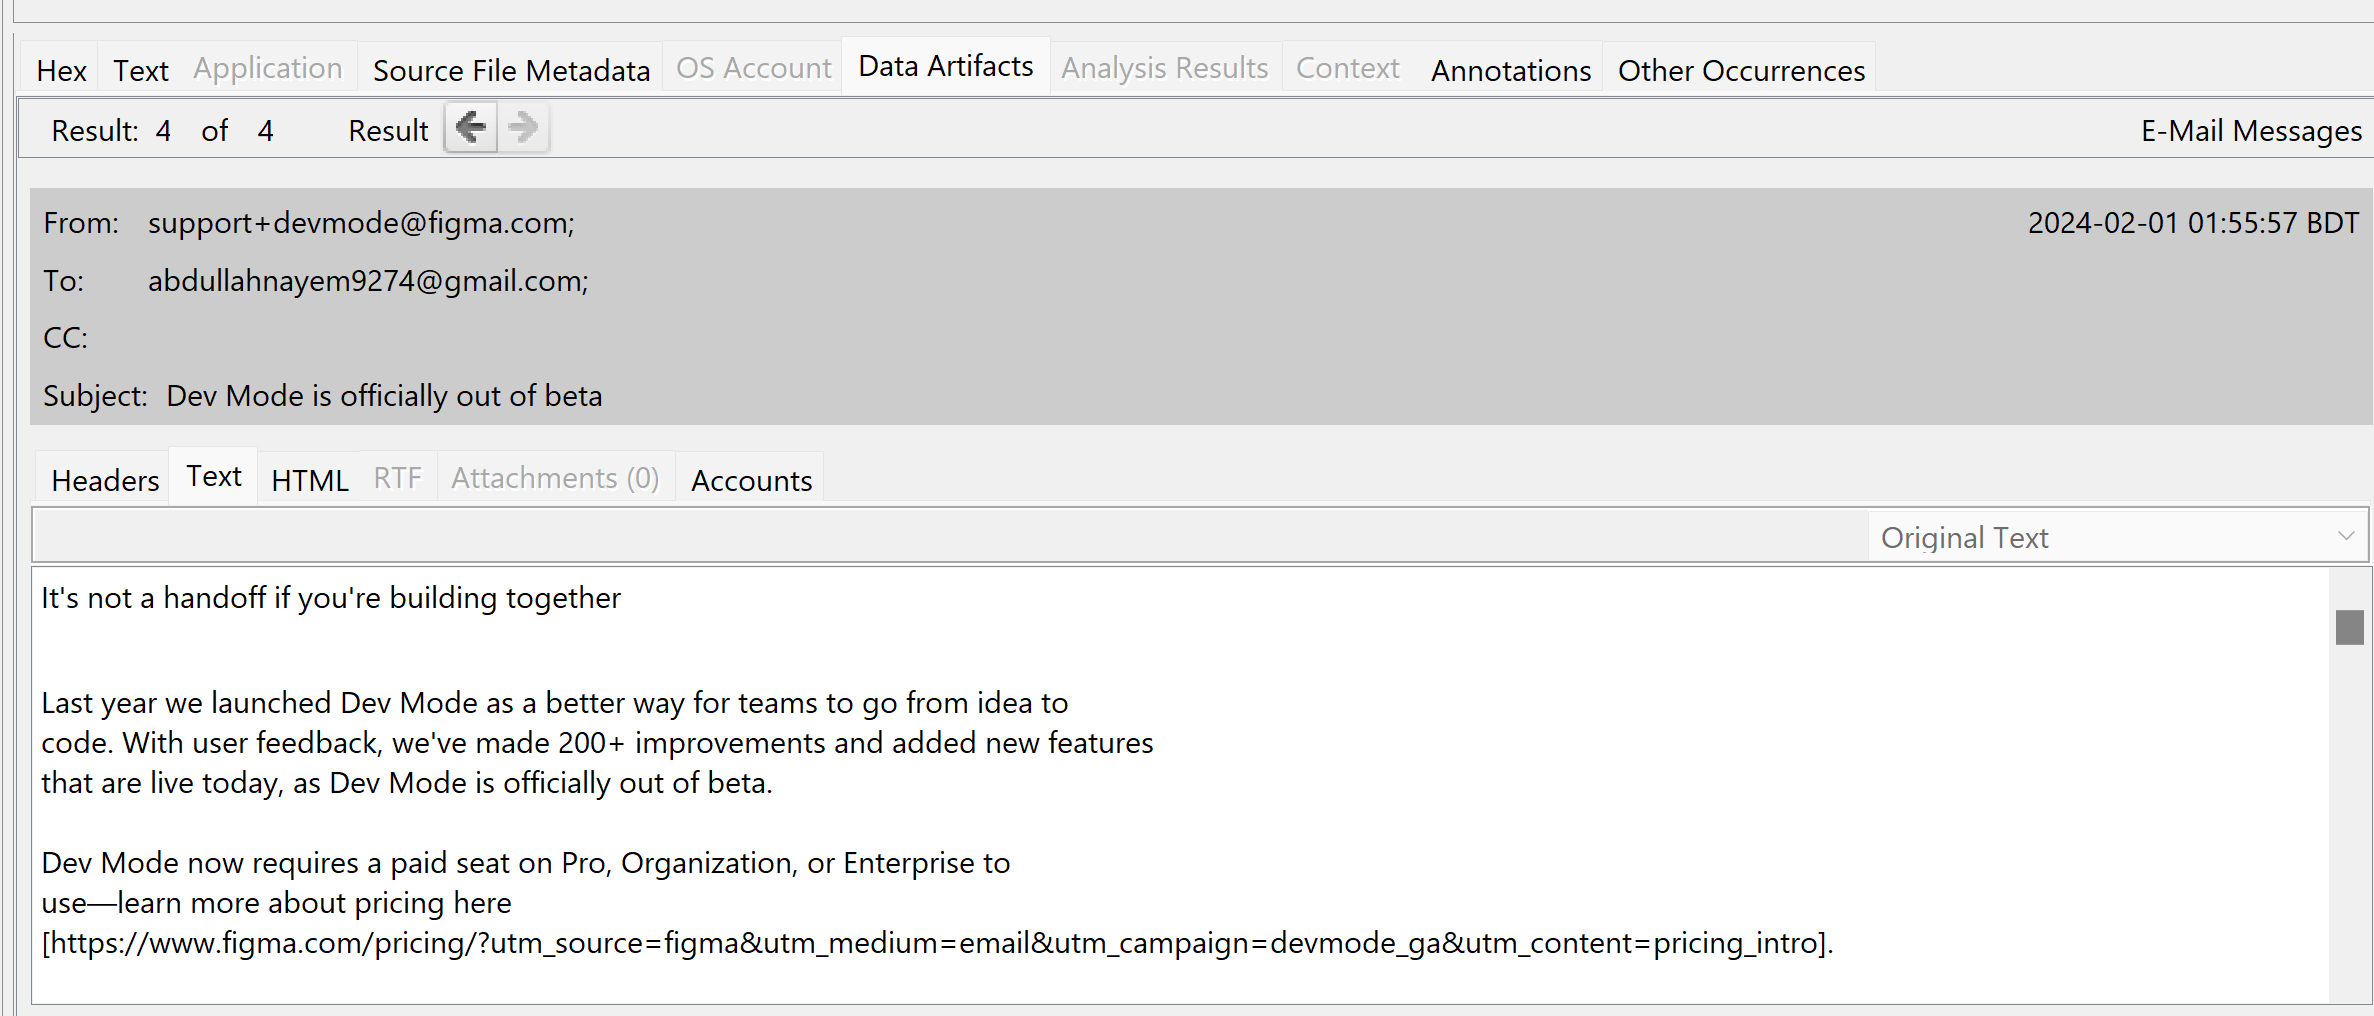
\includegraphics[width=0.75\textwidth]{3/3.9/Details of an email text version.png}
\end{center}

We can also see the details of a selected email in the bottom part of the result.
\begin{center}
    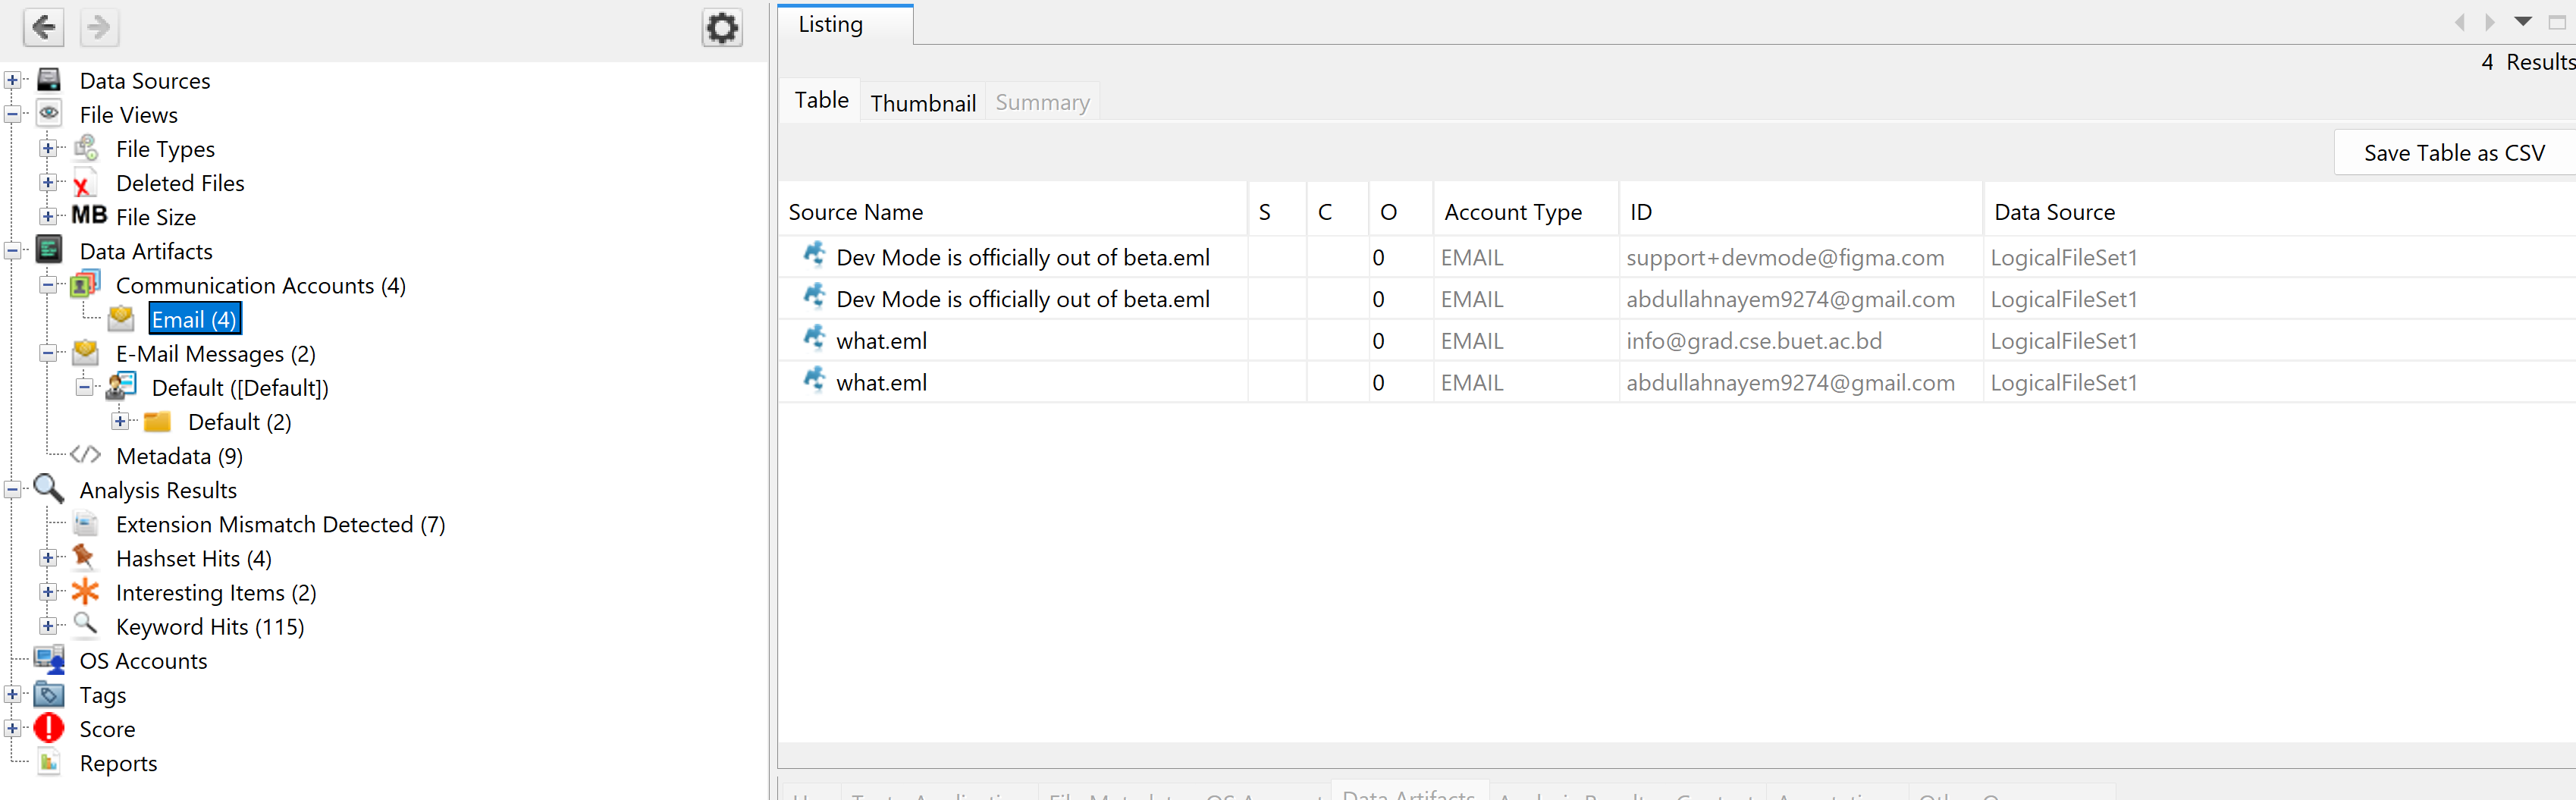
\includegraphics[width=0.75\textwidth]{3/3.9/Email Accounts.png}
\end{center}
From \texttt{Data Artifacts > Communication Accounts > Email}, we can view the email accounts that have been used in the emails identified by the module.

\subsection{Encryption Detection}
The Encryption Detection Module is created to find files that might be encrypted or password-protected. It does this by using both general calculations of randomness and customized tests for different types of files.

\subsubsection*{Results}
\begin{center}
    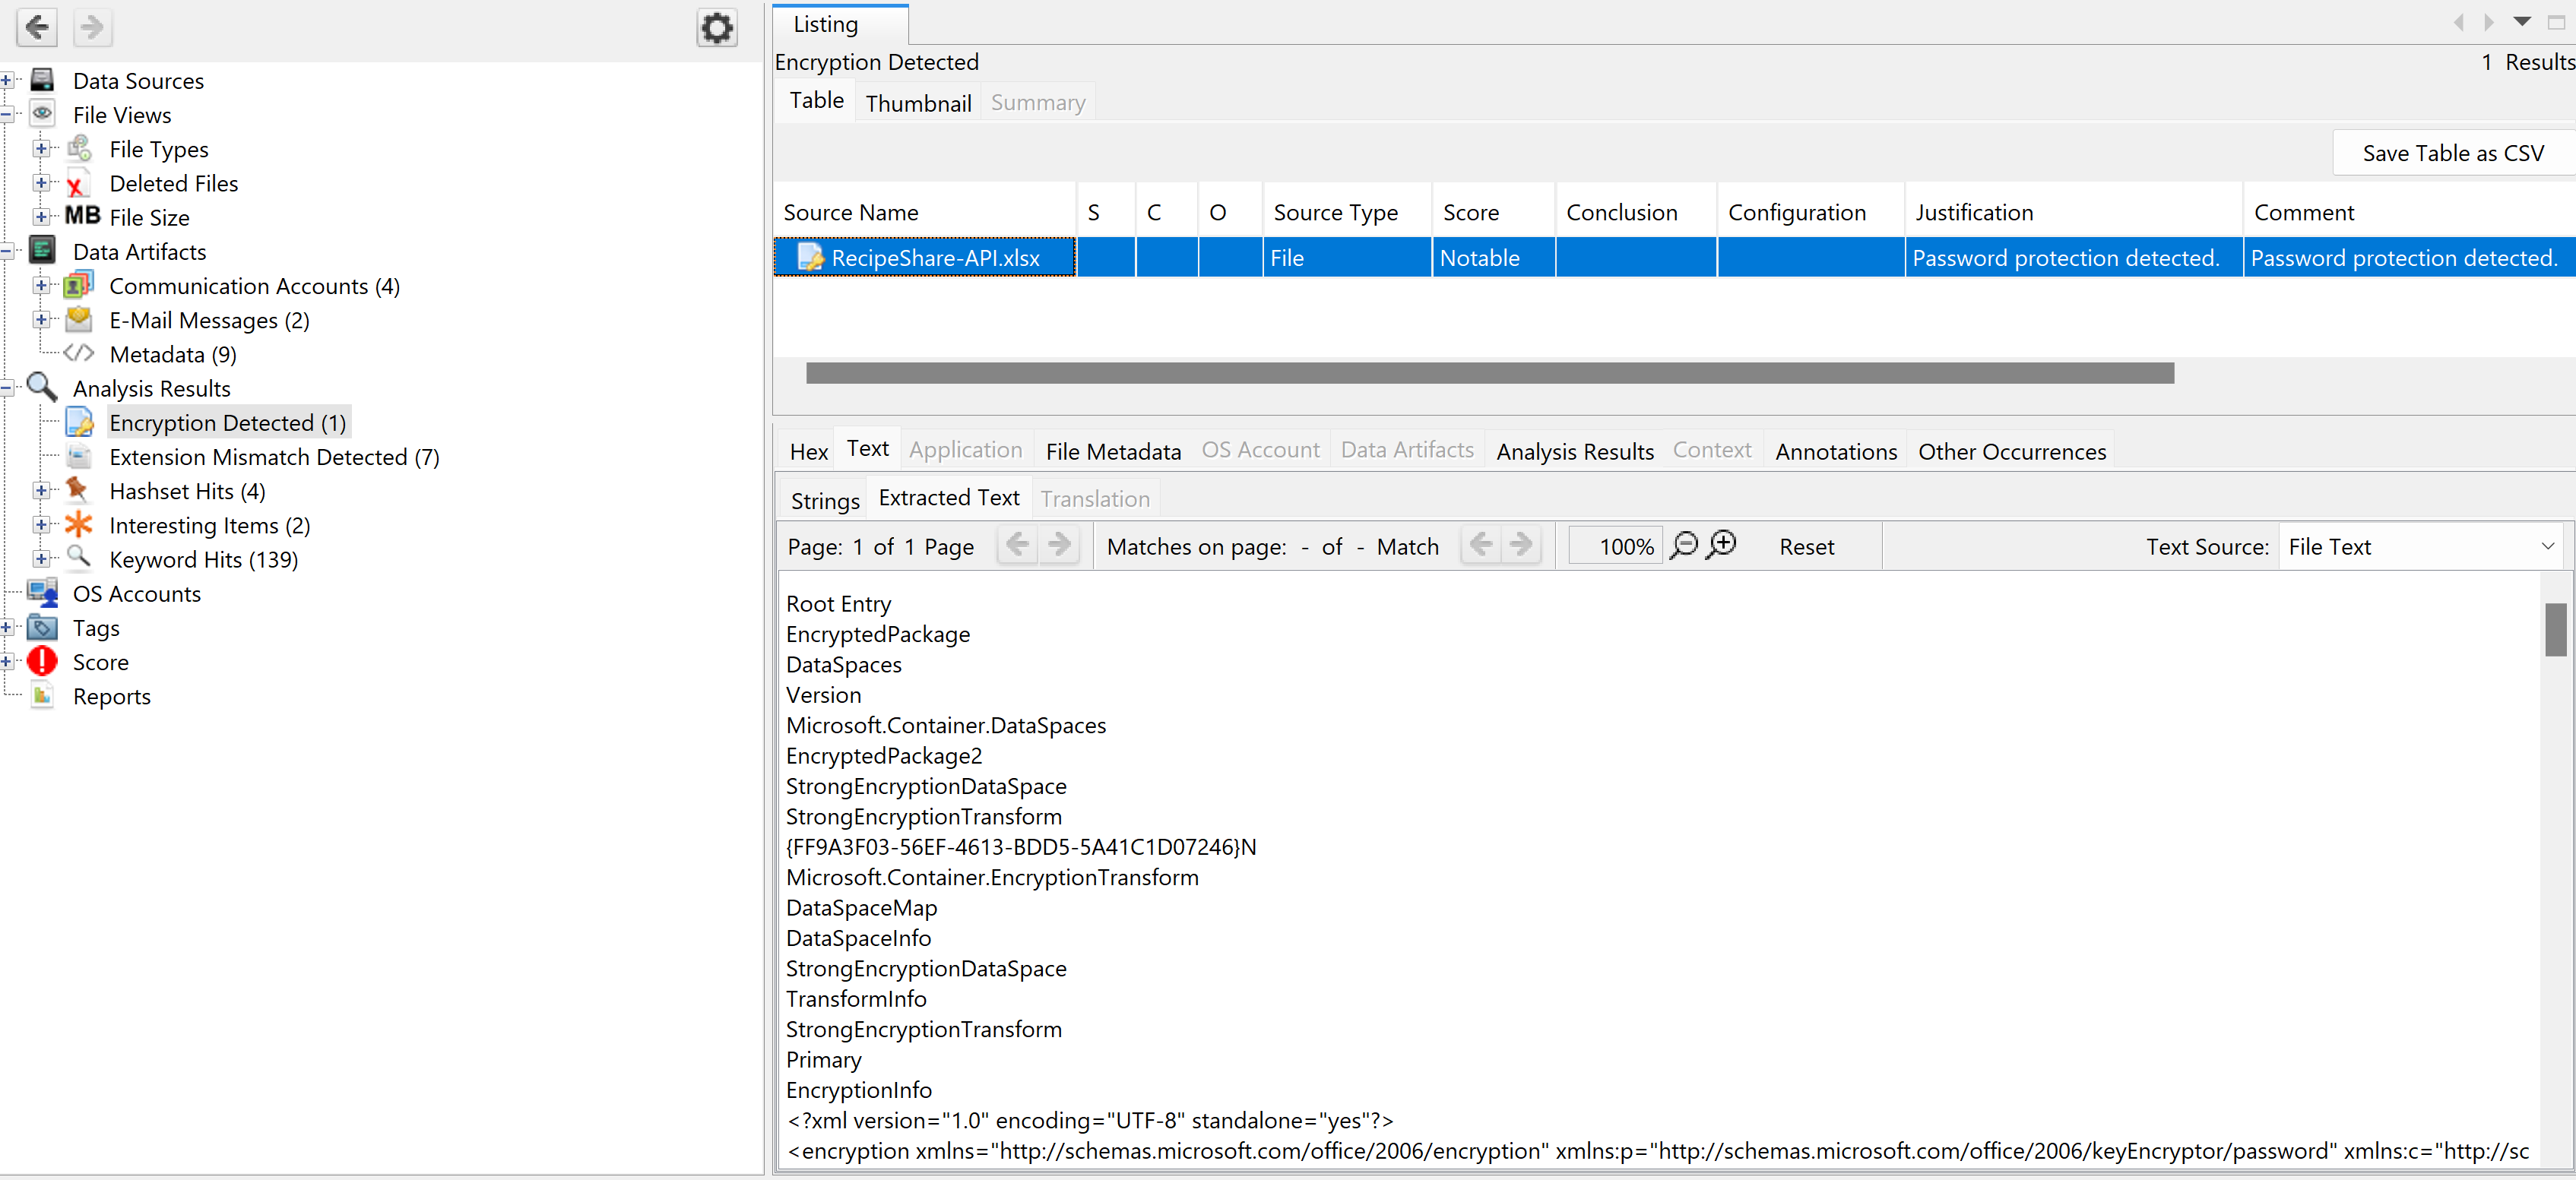
\includegraphics[width=0.75\textwidth]{3/3.10/Results of Encryption Detection ingest module.png}
\end{center}

After executing the "Encryption Detection" ingest module, the outcomes can be observed in \texttt{Analysis Results > Encryption Detection}. one file has been recognized as requiring a password for access.

\subsection{PhotoRec Carver}
The PhotoRec Carver module retrieves files from the unallocated space within the data source and sends them for further processing. This assists users in uncovering additional data about previously deleted files on the device. These files are found in areas of the device's storage that appear empty. Users can customize the module's runtime settings to choose whether to retain corrupted files and specify which file types to include or exclude.
\begin{center}
    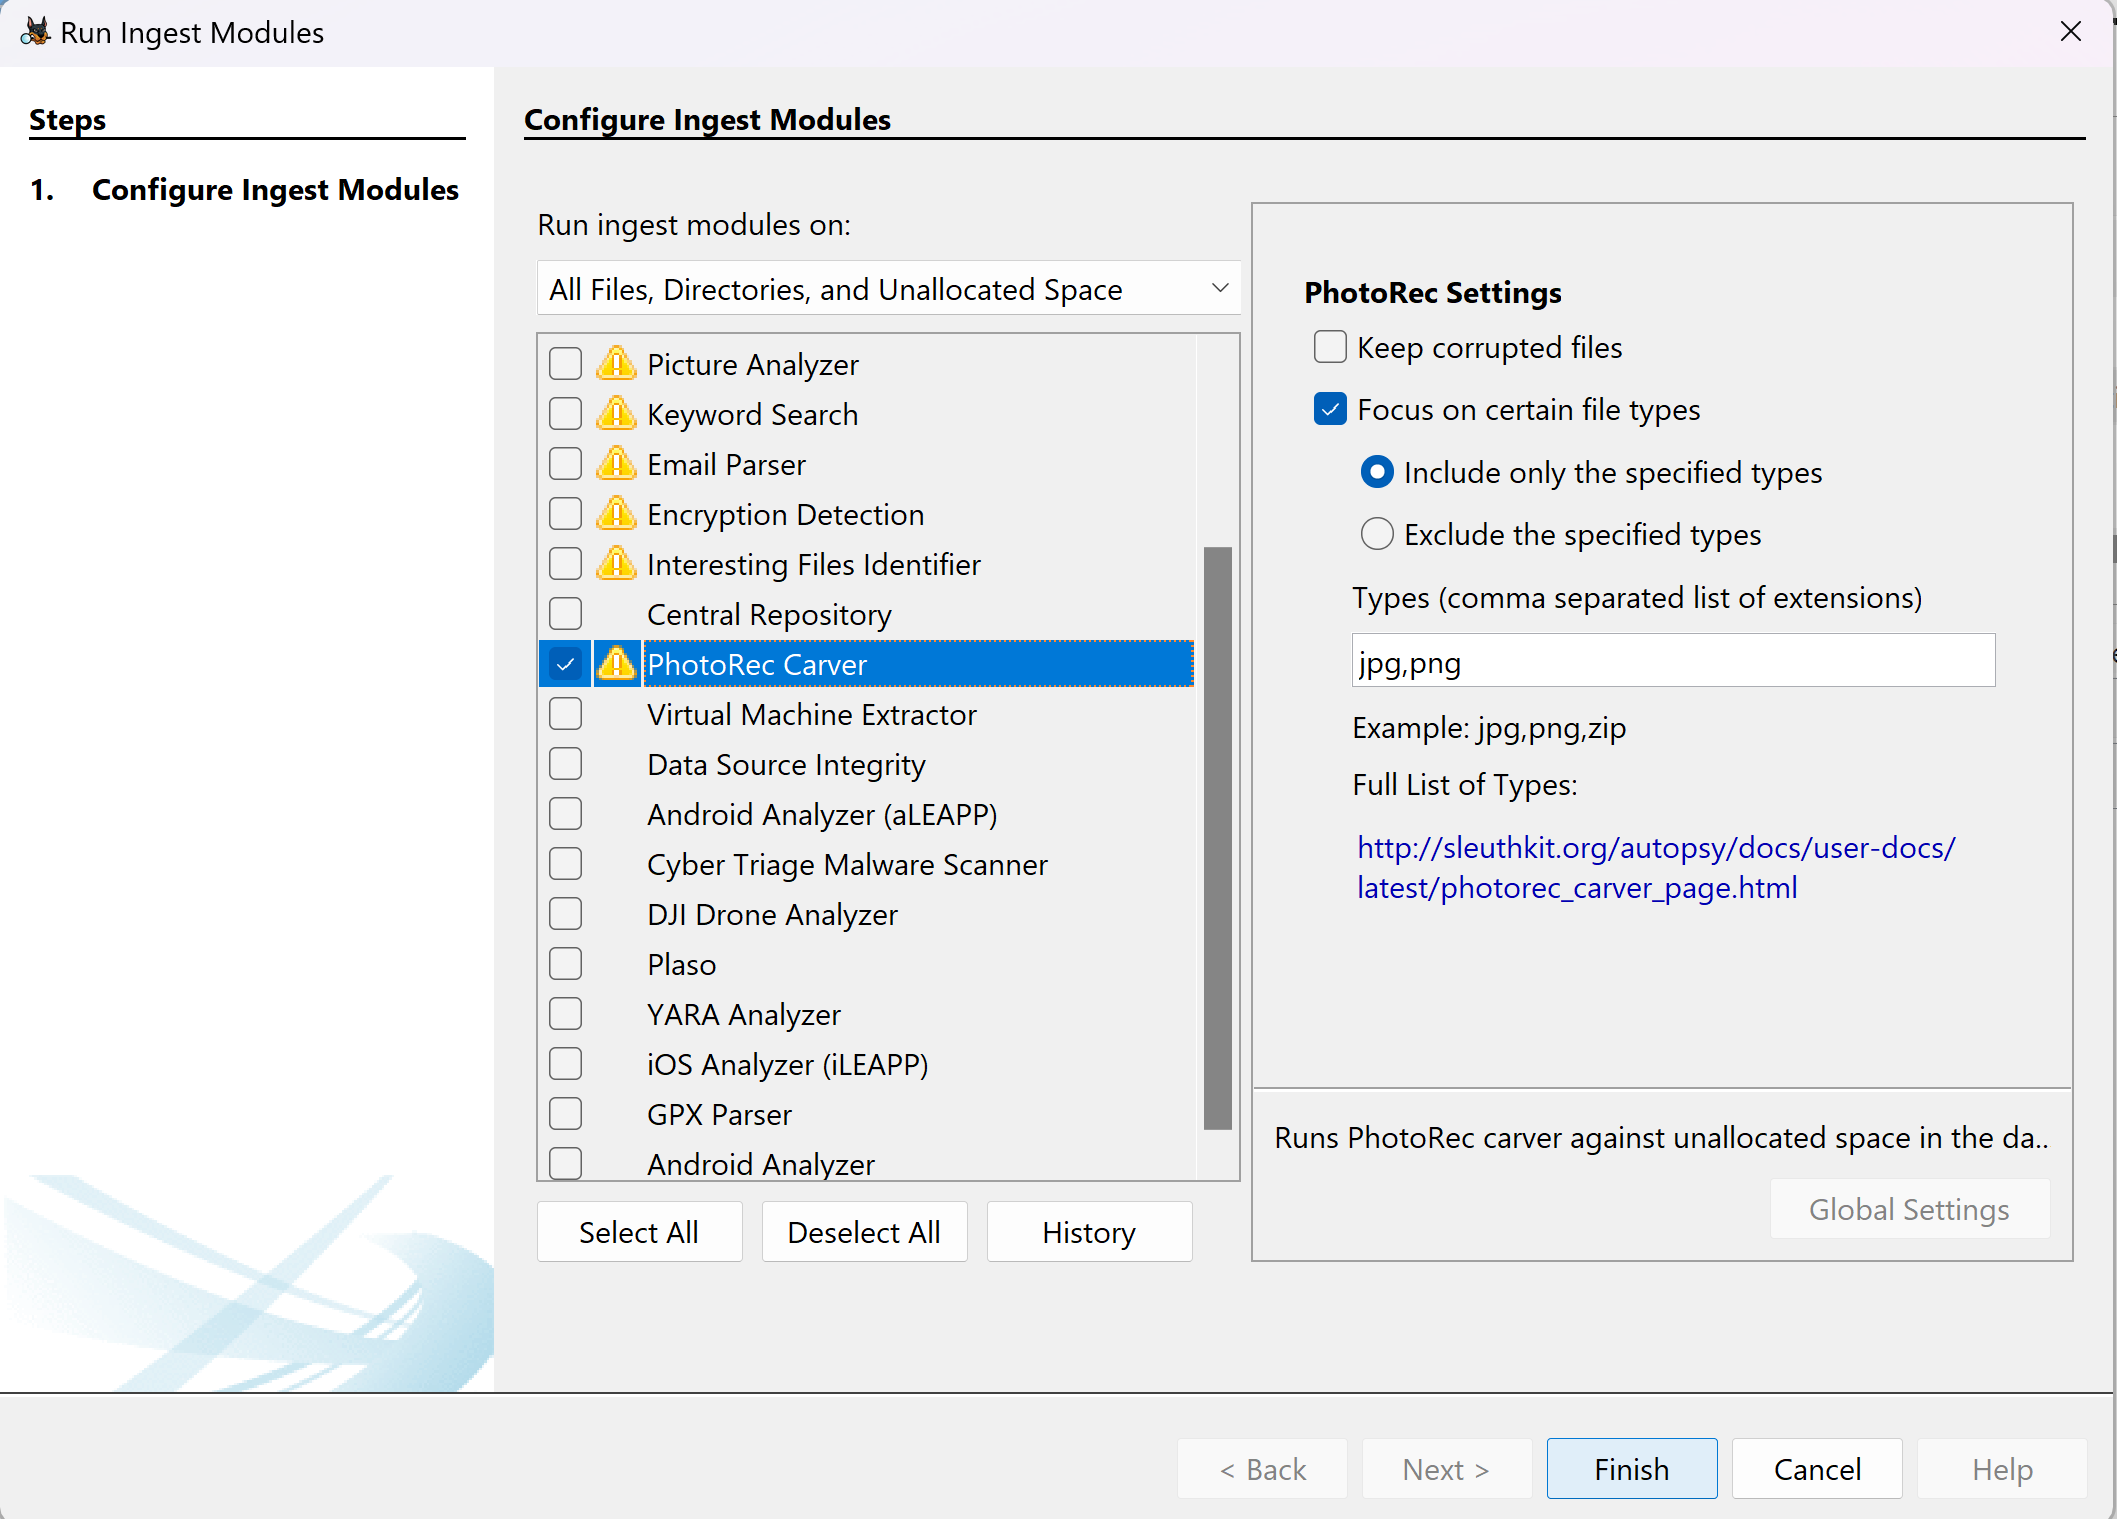
\includegraphics[width=0.75\textwidth]{3/3.11/PhotoRec Carver Settings.png}
\end{center}


\subsubsection*{Results}
The results of carving show up on the tree under the appropriate data source with the heading (CarvedFiles)
\begin{center}
    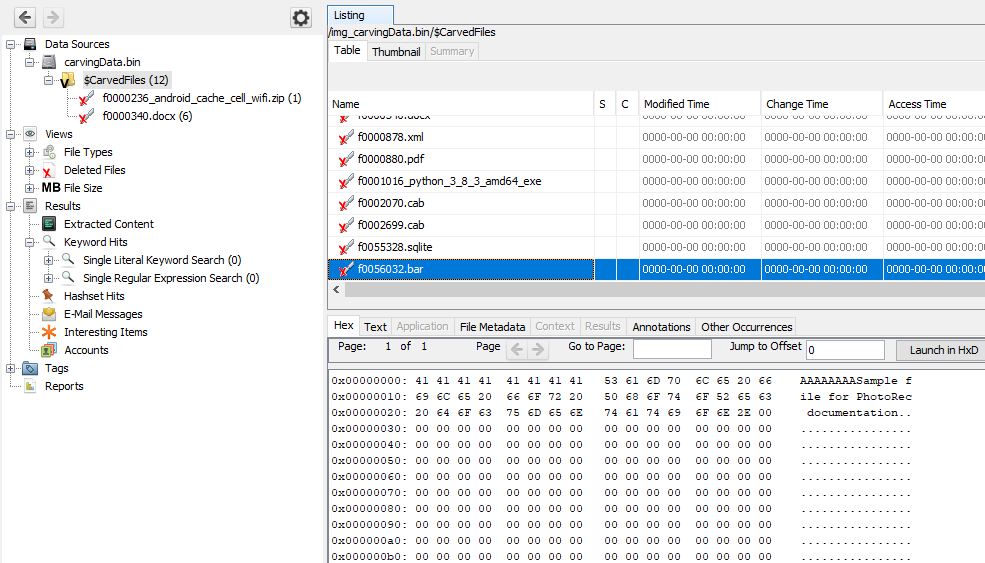
\includegraphics[width=0.75\textwidth]{3/3.11/PhotoRec Carver Results.png}
\end{center}

\section{Specialize Views}
\subsection{Images/Video Gallery}
The Image Gallery feature in Autopsy assists in investigations related to images and videos. It categorizes photos into folders and properties, simplifying the management of large collections and focusing on significant content. It allows for immediate image viewing during ingestion, eliminating the need to wait for the entire process to finish.

\begin{center}
    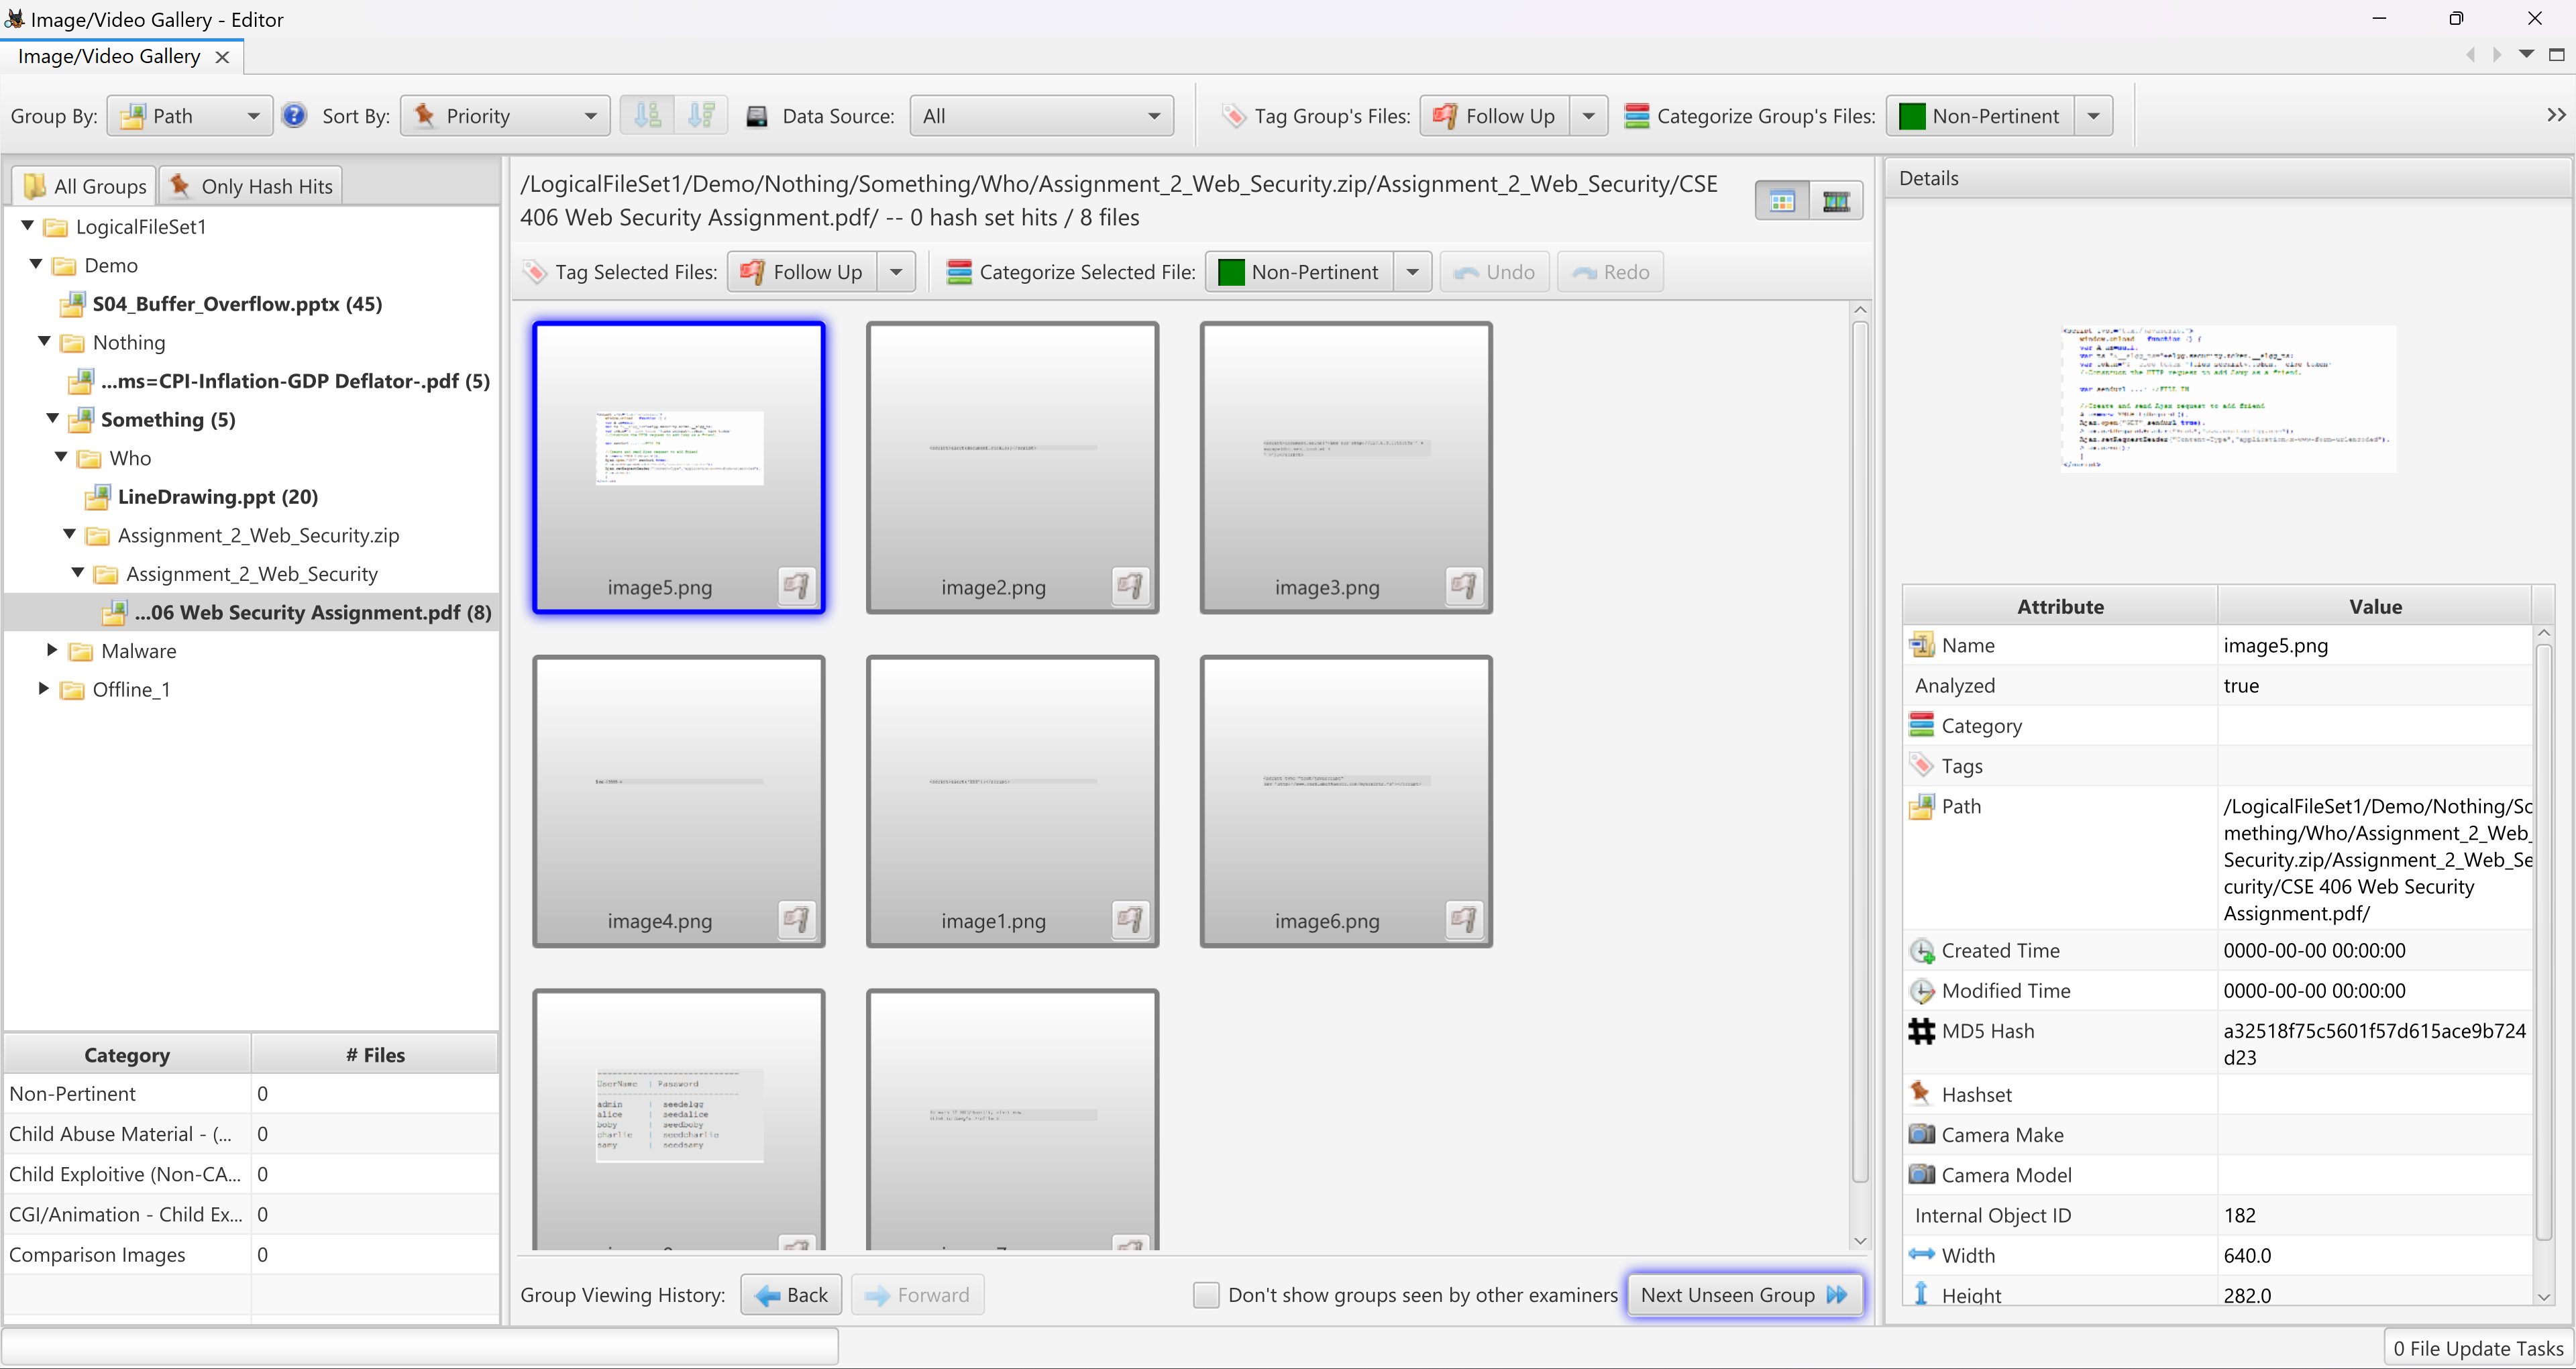
\includegraphics[width=0.75\textwidth]{4/4.1/Image Gallery.png}
\end{center}

\subsection{Timeline}

Autopsy's Timeline is a robust digital forensics tool that logs important events like web activity, external device connections, EXIF photo additions, and their connections with file system modifications.

To fully utilize the Timeline feature, it's essential to run the Hash Lookup, Recent Activity, and Picture Analyzer modules beforehand.

The Timeline tool is event-based, with each event having a timestamp, category, and description. While each event is distinct, users can manually group them together if needed.

Autopsy's Timeline feature gathers and organizes data from various sources into event types, such as for File System Changes (Access, Creation, Modification, Deletion).

\begin{center}
    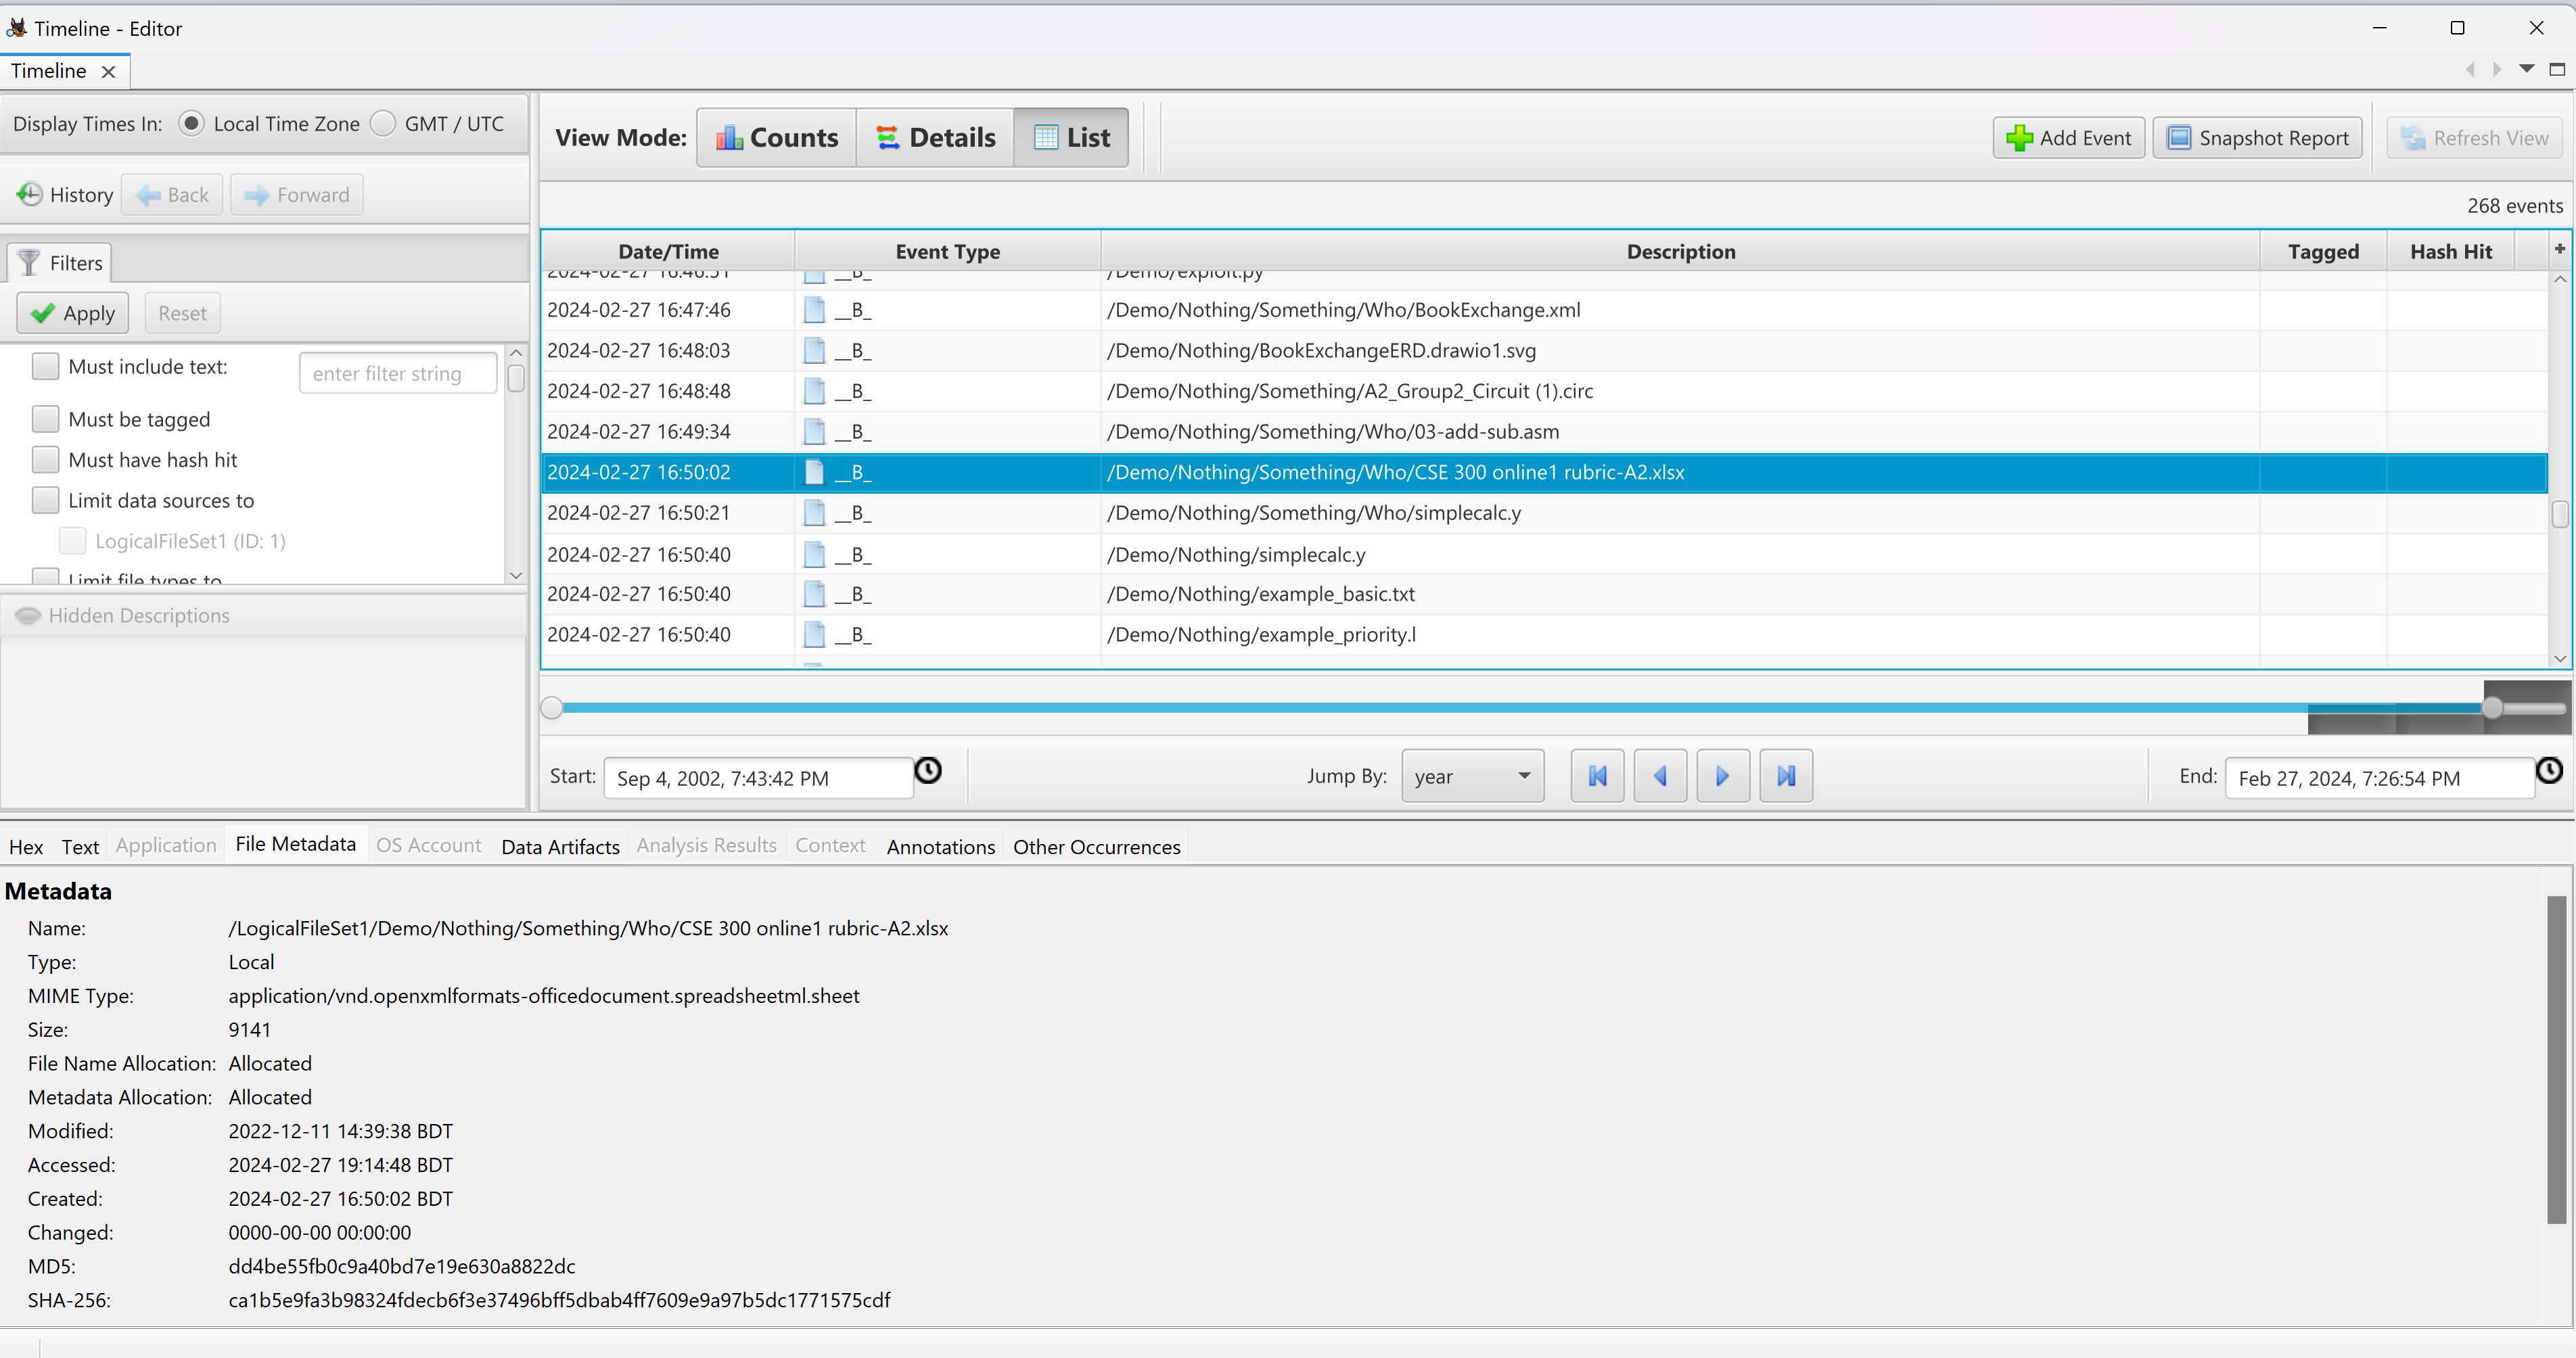
\includegraphics[width=0.75\textwidth]{4/4.2/Timeline View-1.png}
\end{center}

\begin{center}
    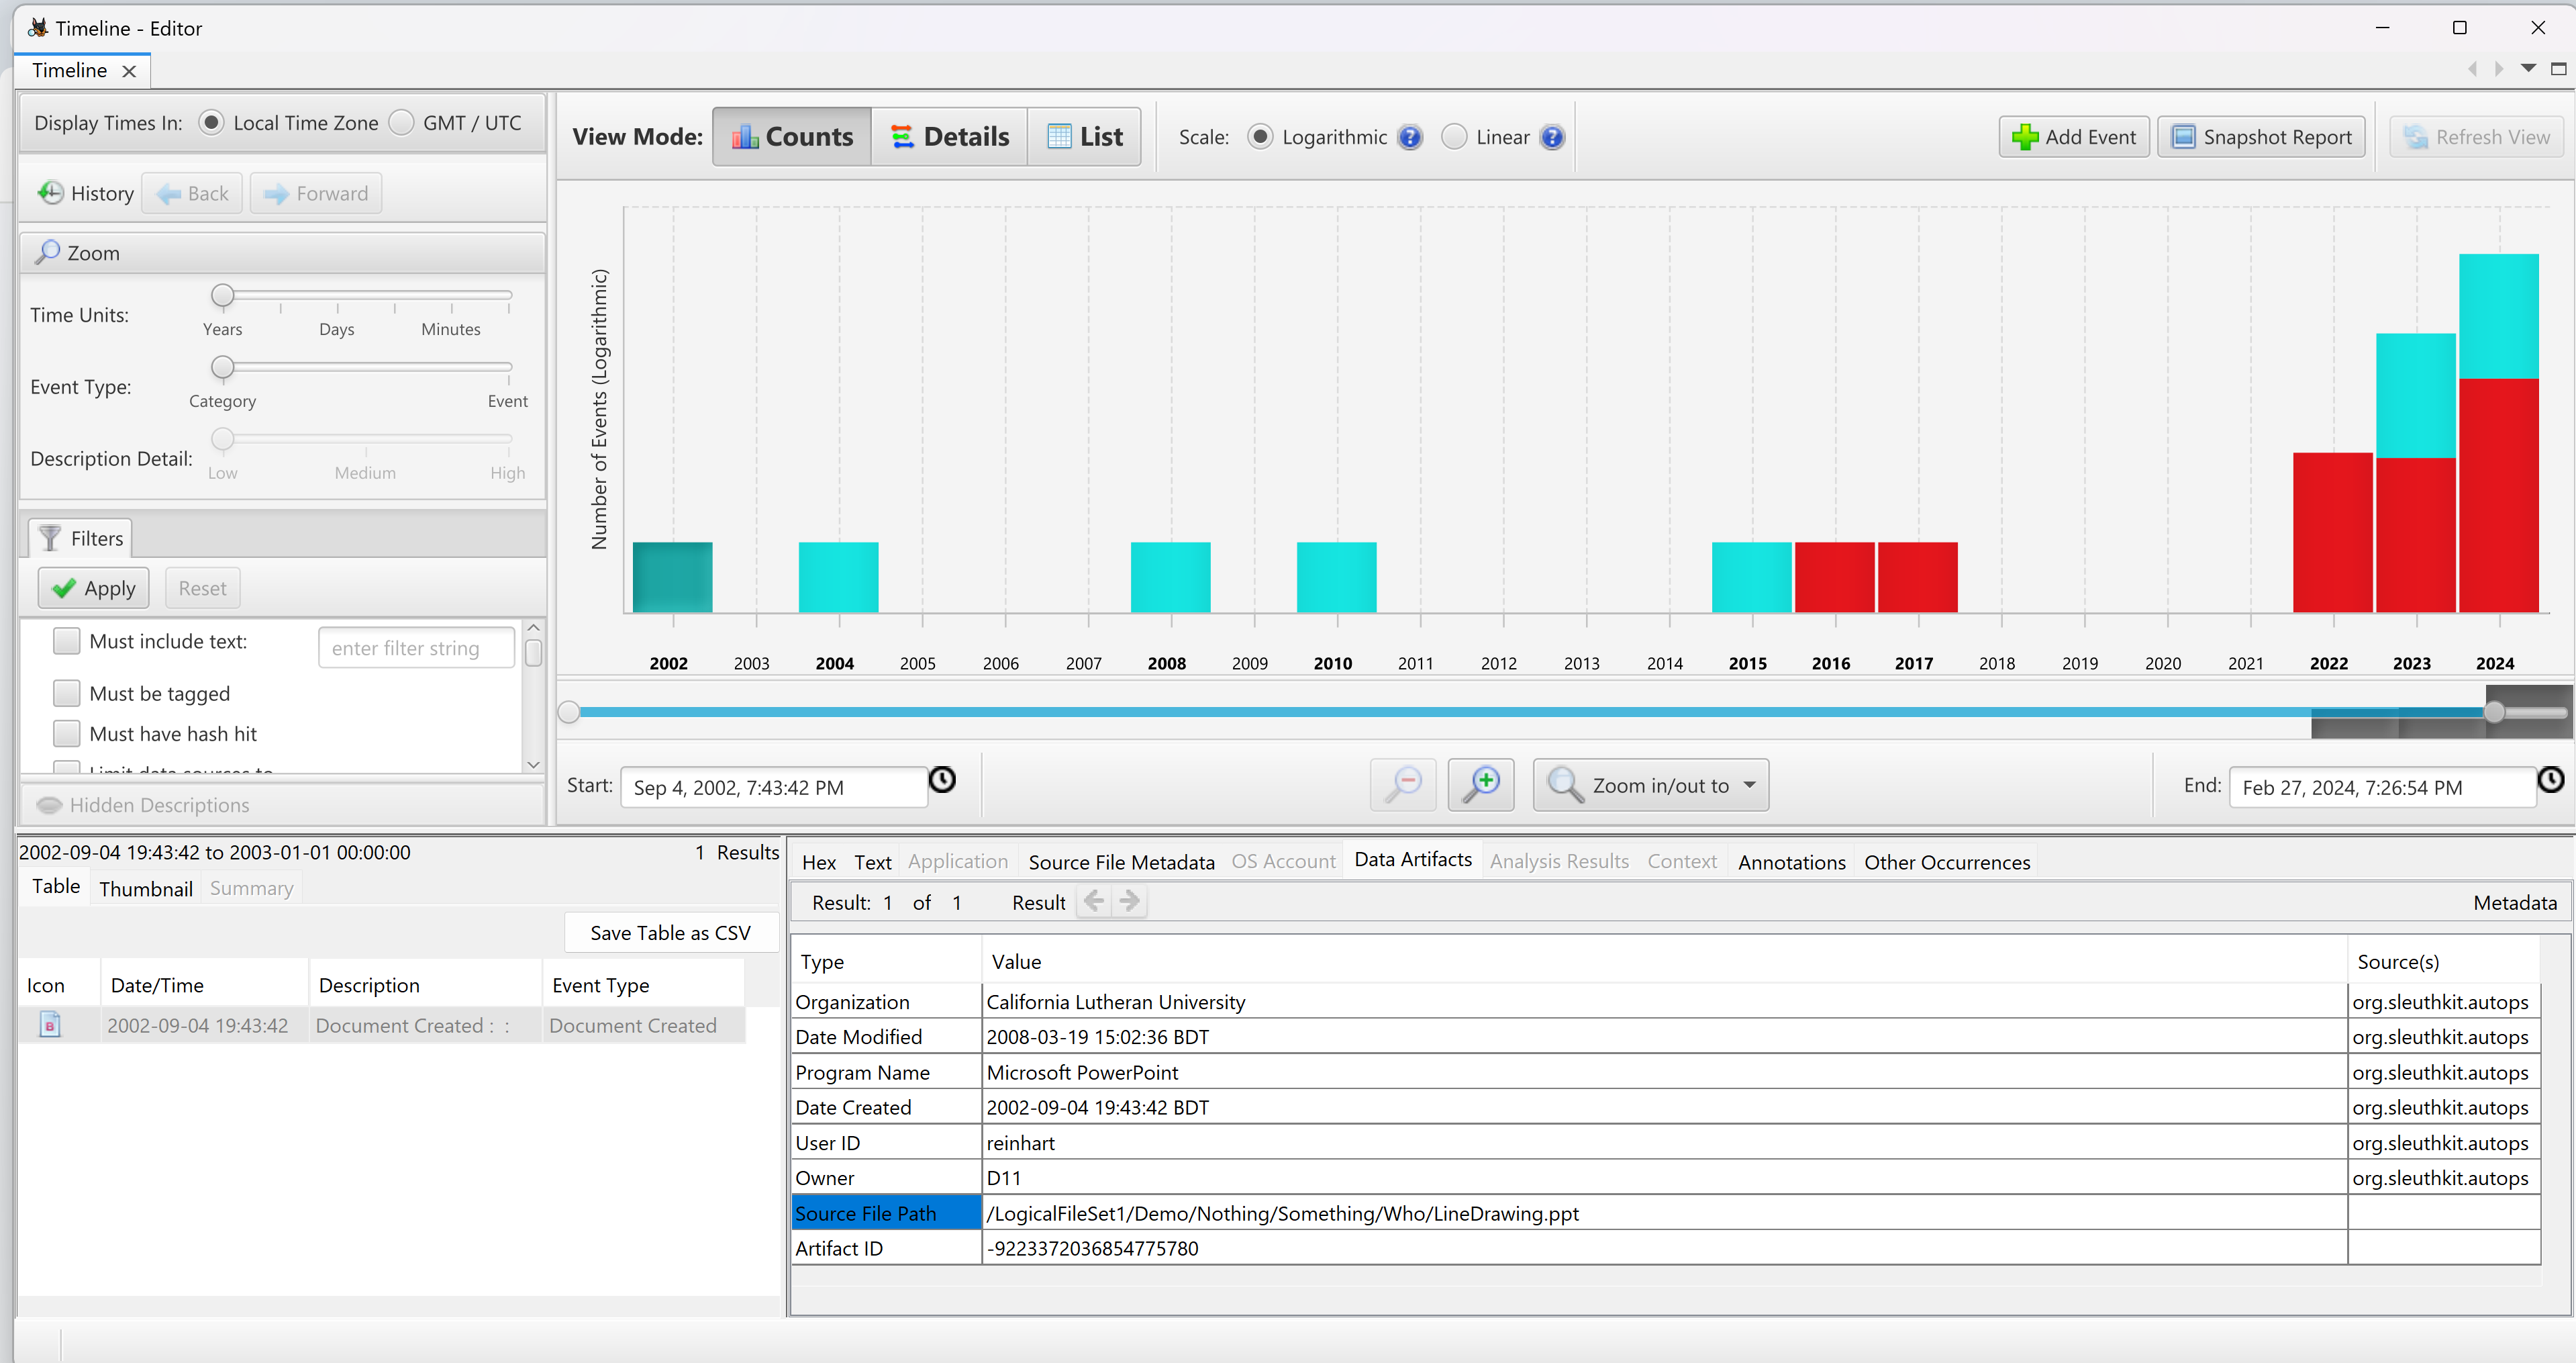
\includegraphics[width=0.75\textwidth]{4/4.2/Timeline View-2.png}
\end{center}

\subsection{File Deletion and Recovery on USB Pendrives}
 In this exploration, we delve into the intricate process of deleting files from USB pendrives and subsequently recovering them using Autopsy, a powerful digital forensic tool. We uncover the digital trails left behind after deletion, analyzing metadata such as timestamps and file allocation tables within the Autopsy interface. Furthermore, we navigate through Autopsy's specialized features and modules designed for scanning and retrieving deleted files, providing detailed insights for forensic investigators seeking to extract crucial evidence from USB pendrives.

 Here we will recover and export a file named "47-Collaboration Diagram"(It was previously in our pendrive but we deleted it) to our local machine.

\subsubsection*{Configuring Setup for File Recovery}
\begin{center}
    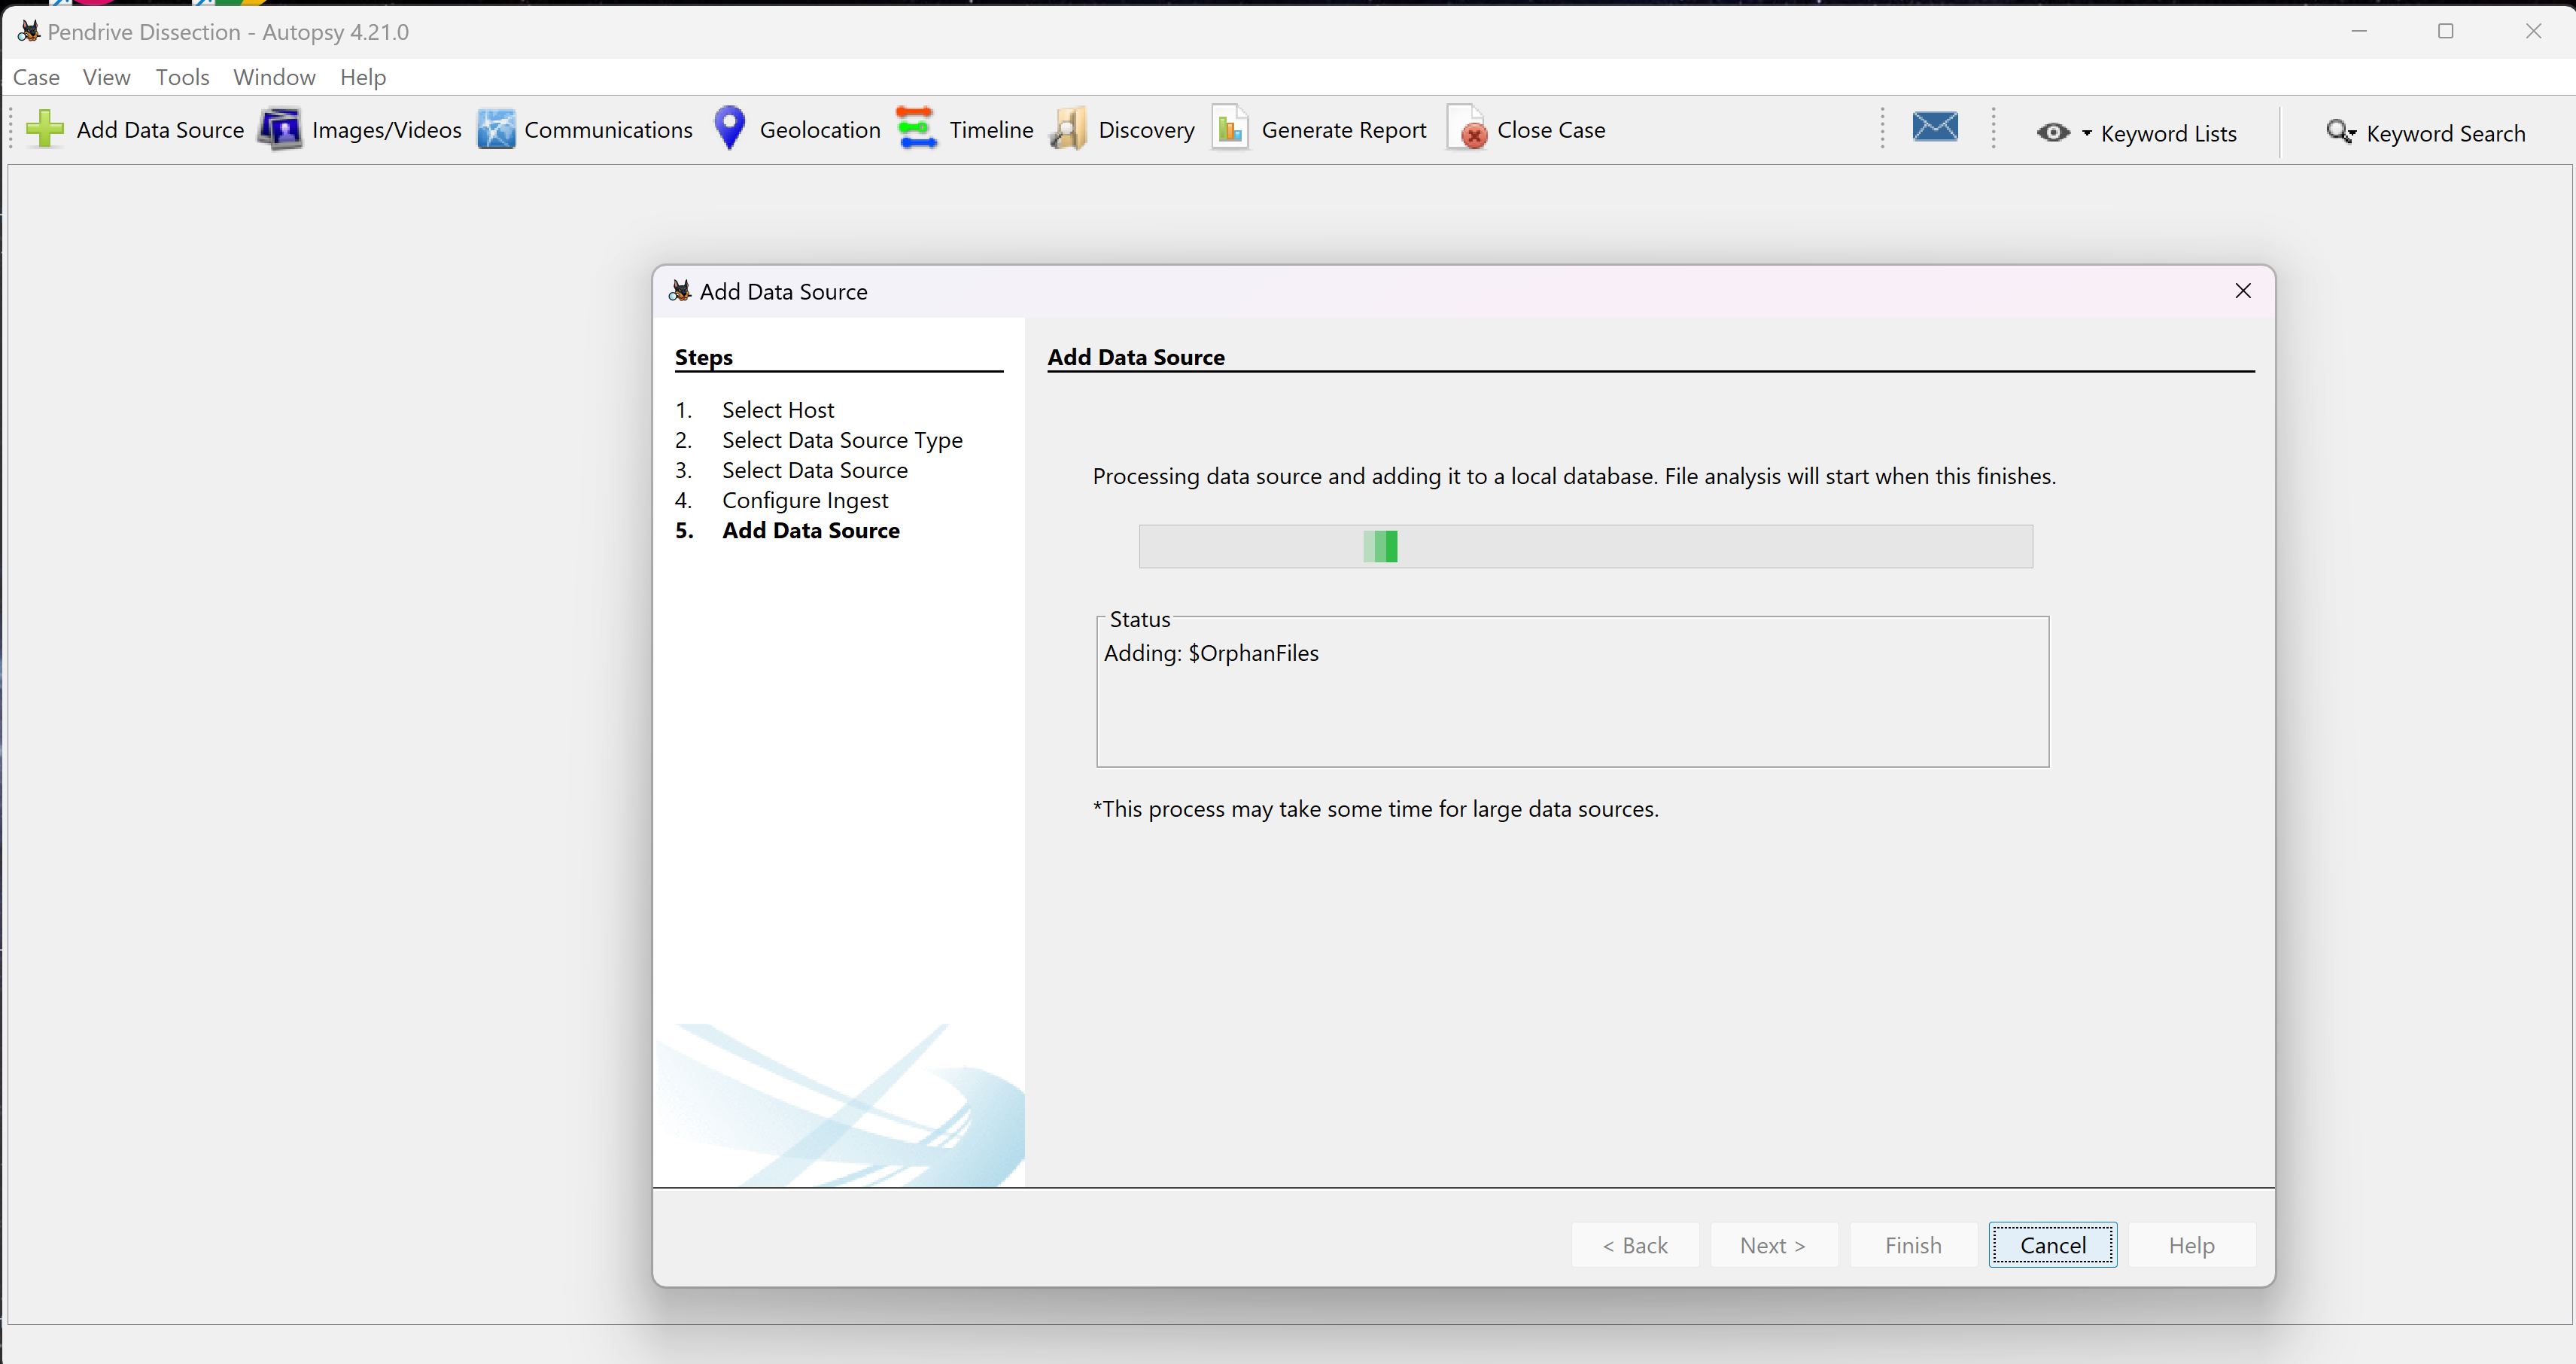
\includegraphics[width=0.75\textwidth]{4.3/Screenshot (414).png}
\end{center}

\begin{center}
    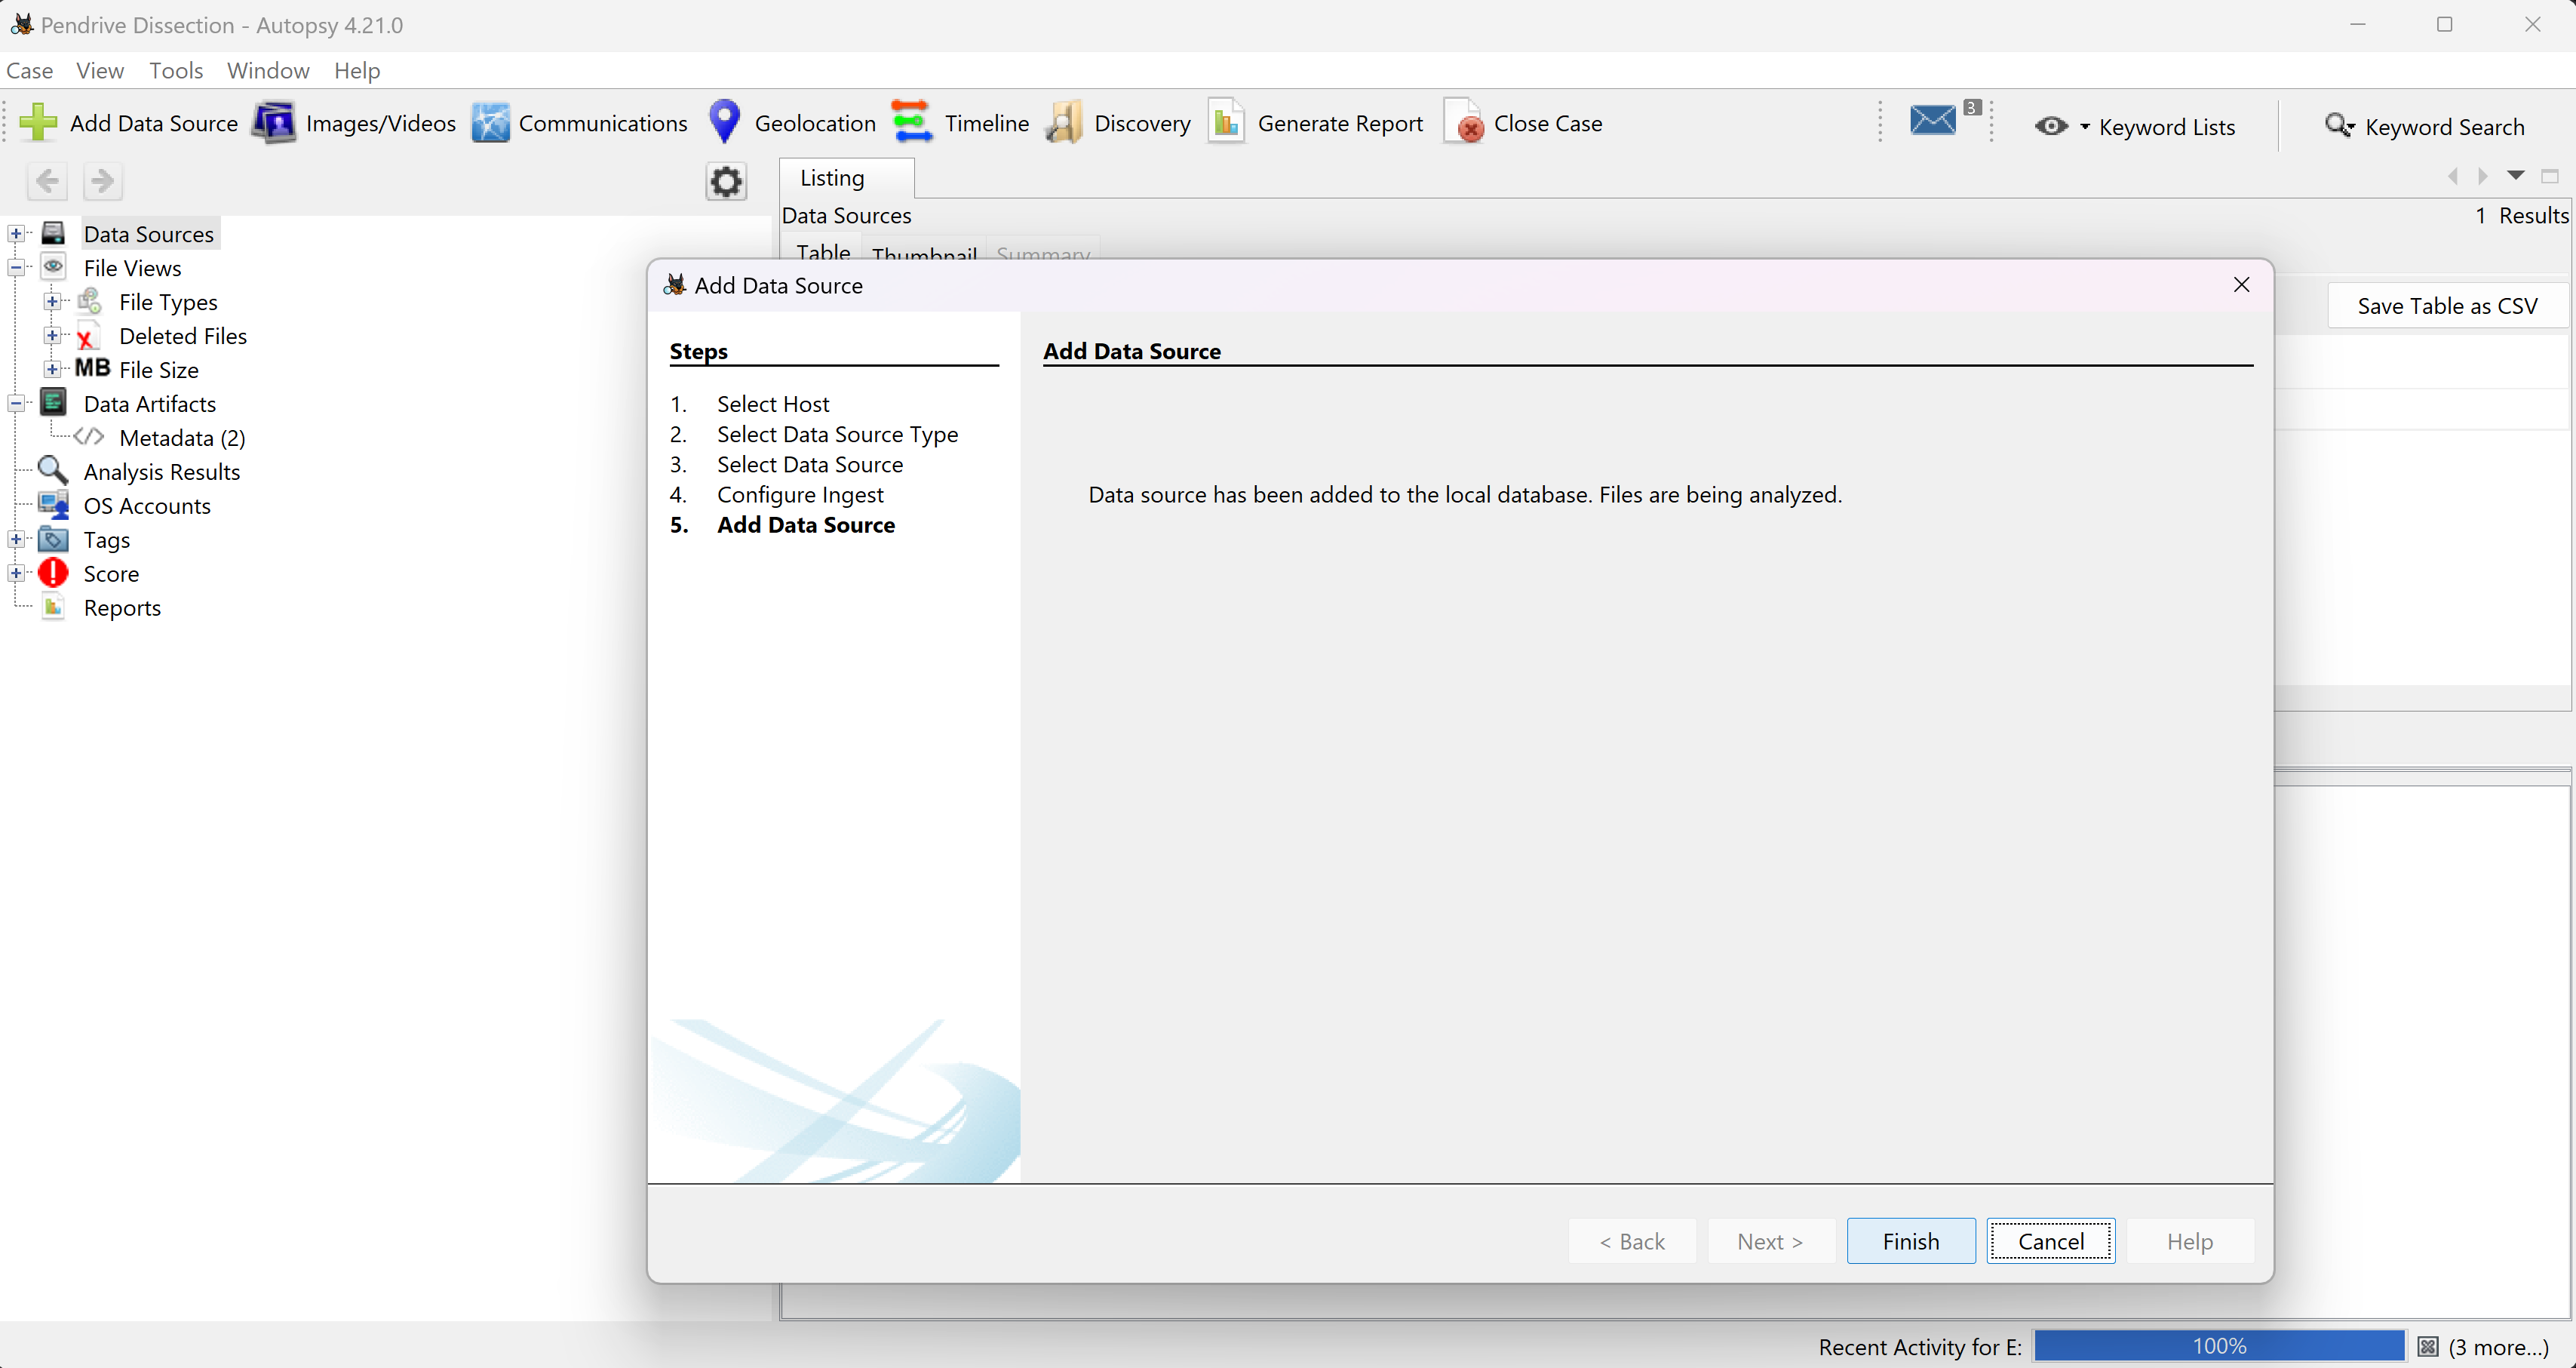
\includegraphics[width=0.75\textwidth]{4.3/Screenshot (415).png}
\end{center}

\subsubsection*{Results}
\begin{center}
    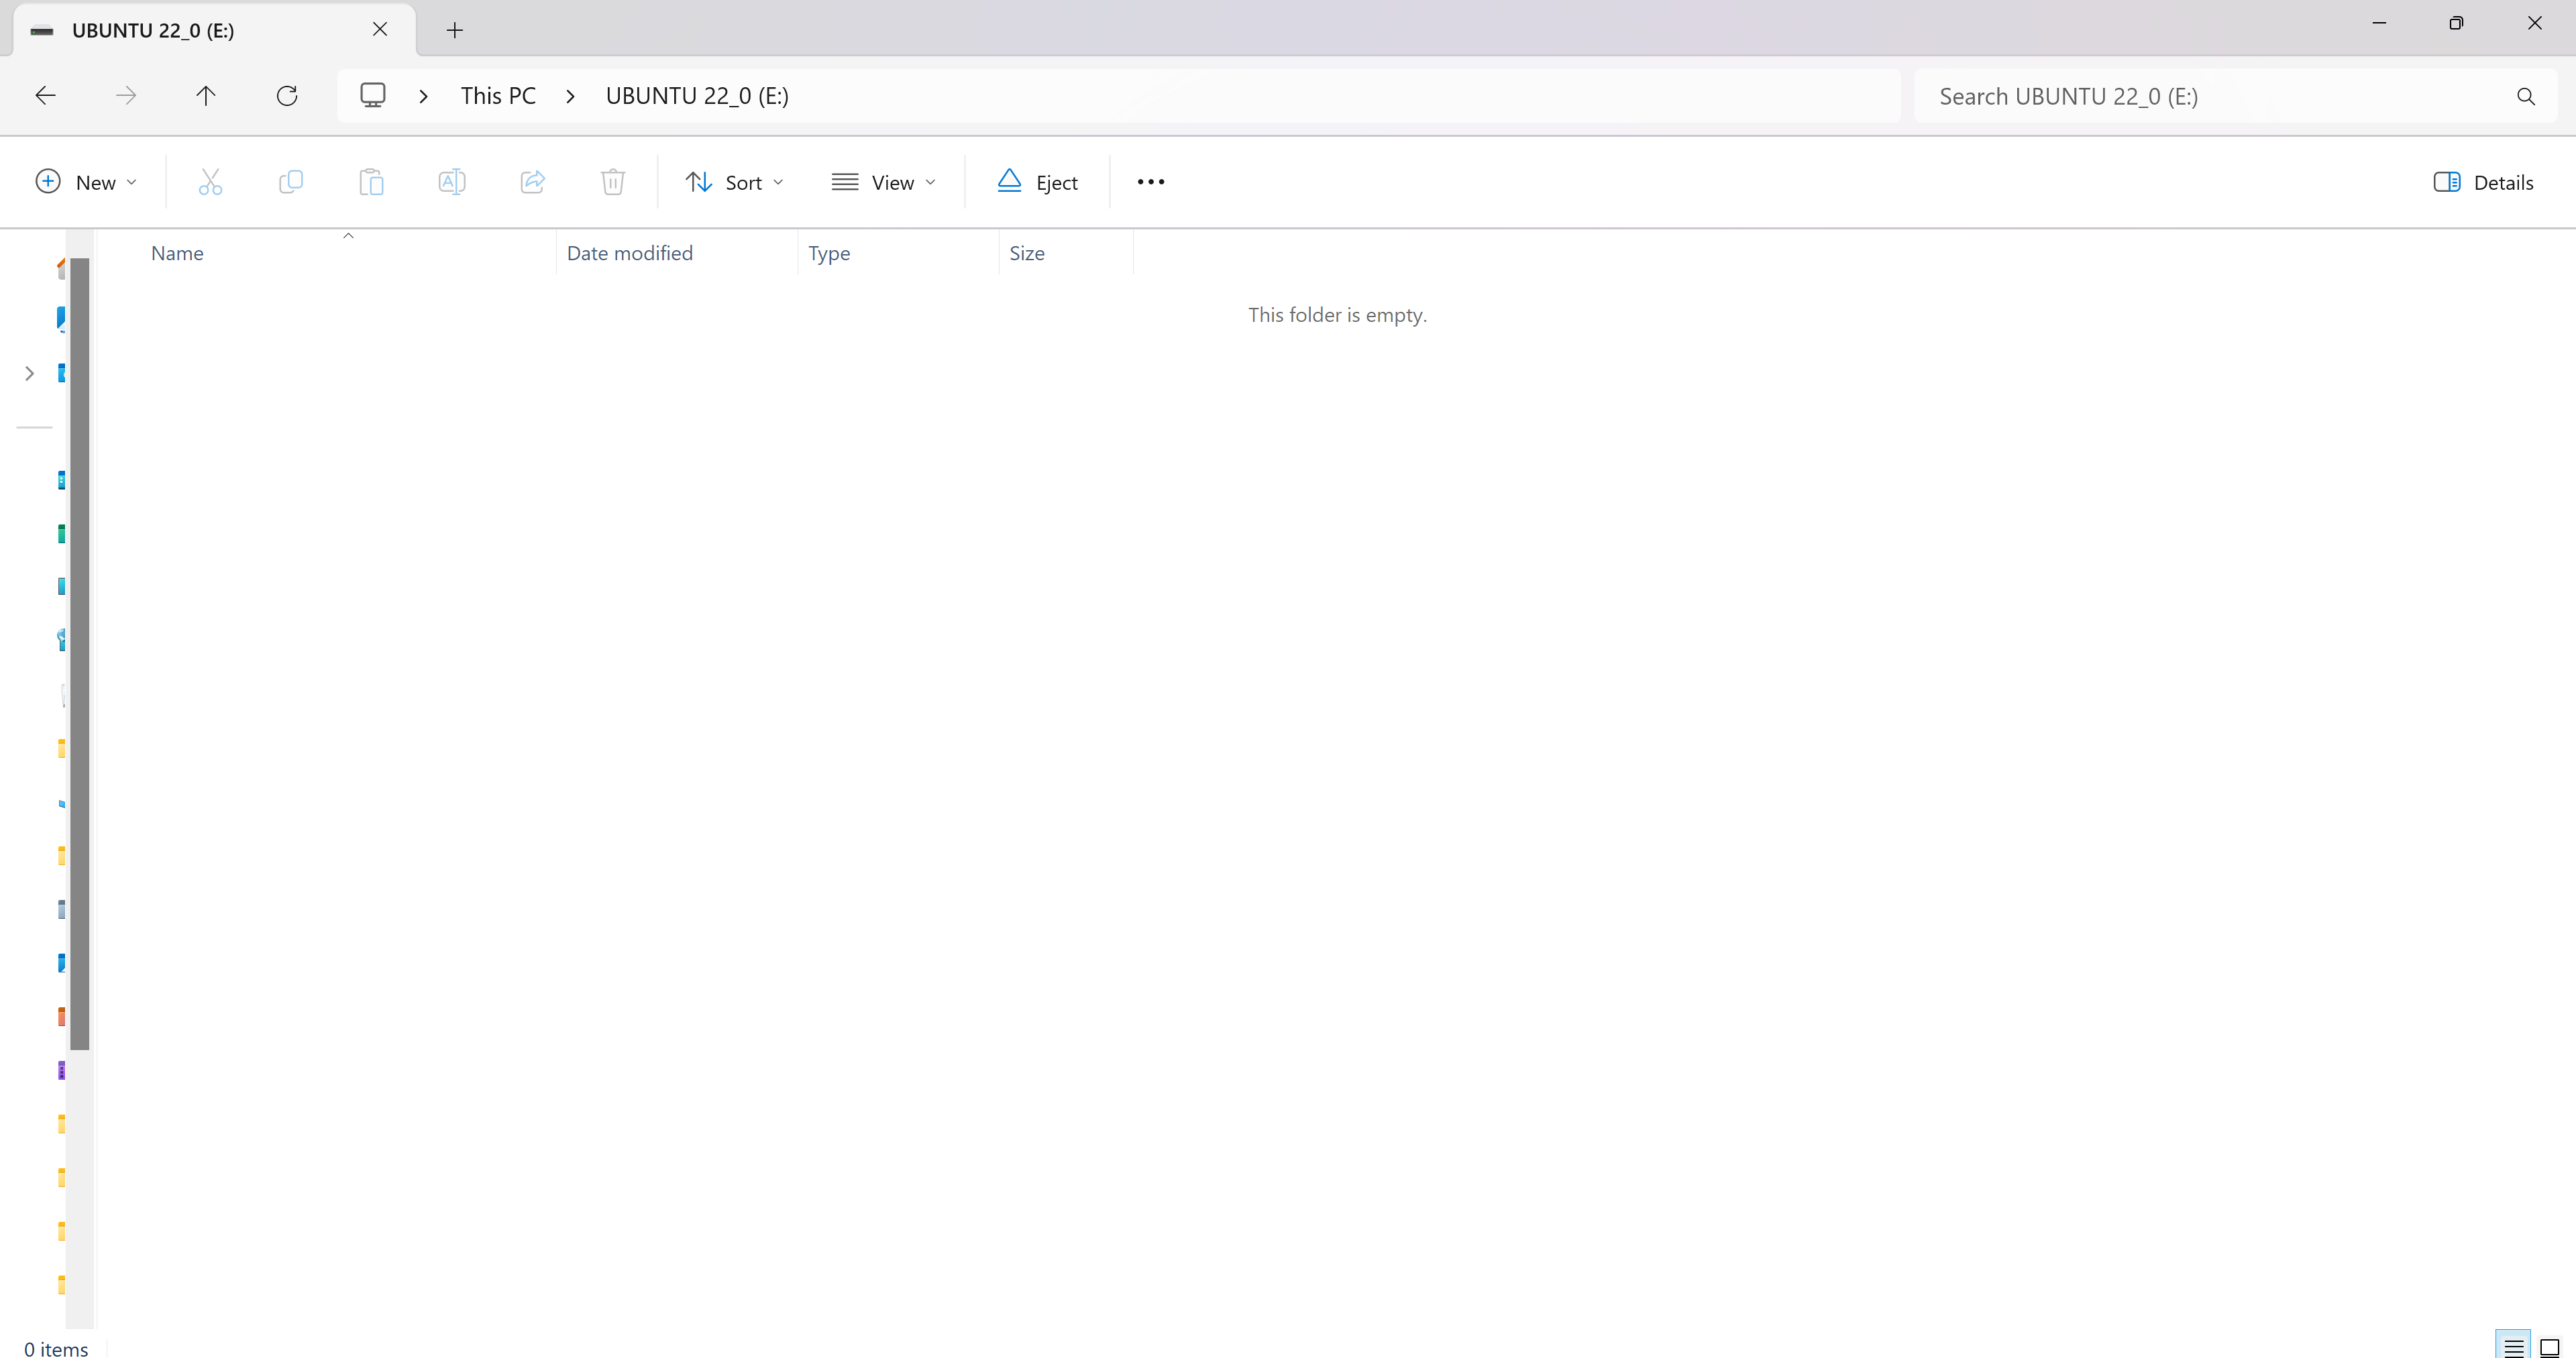
\includegraphics[width=0.75\textwidth]{4.3/Screenshot (416).png}
\end{center}

\begin{center}
    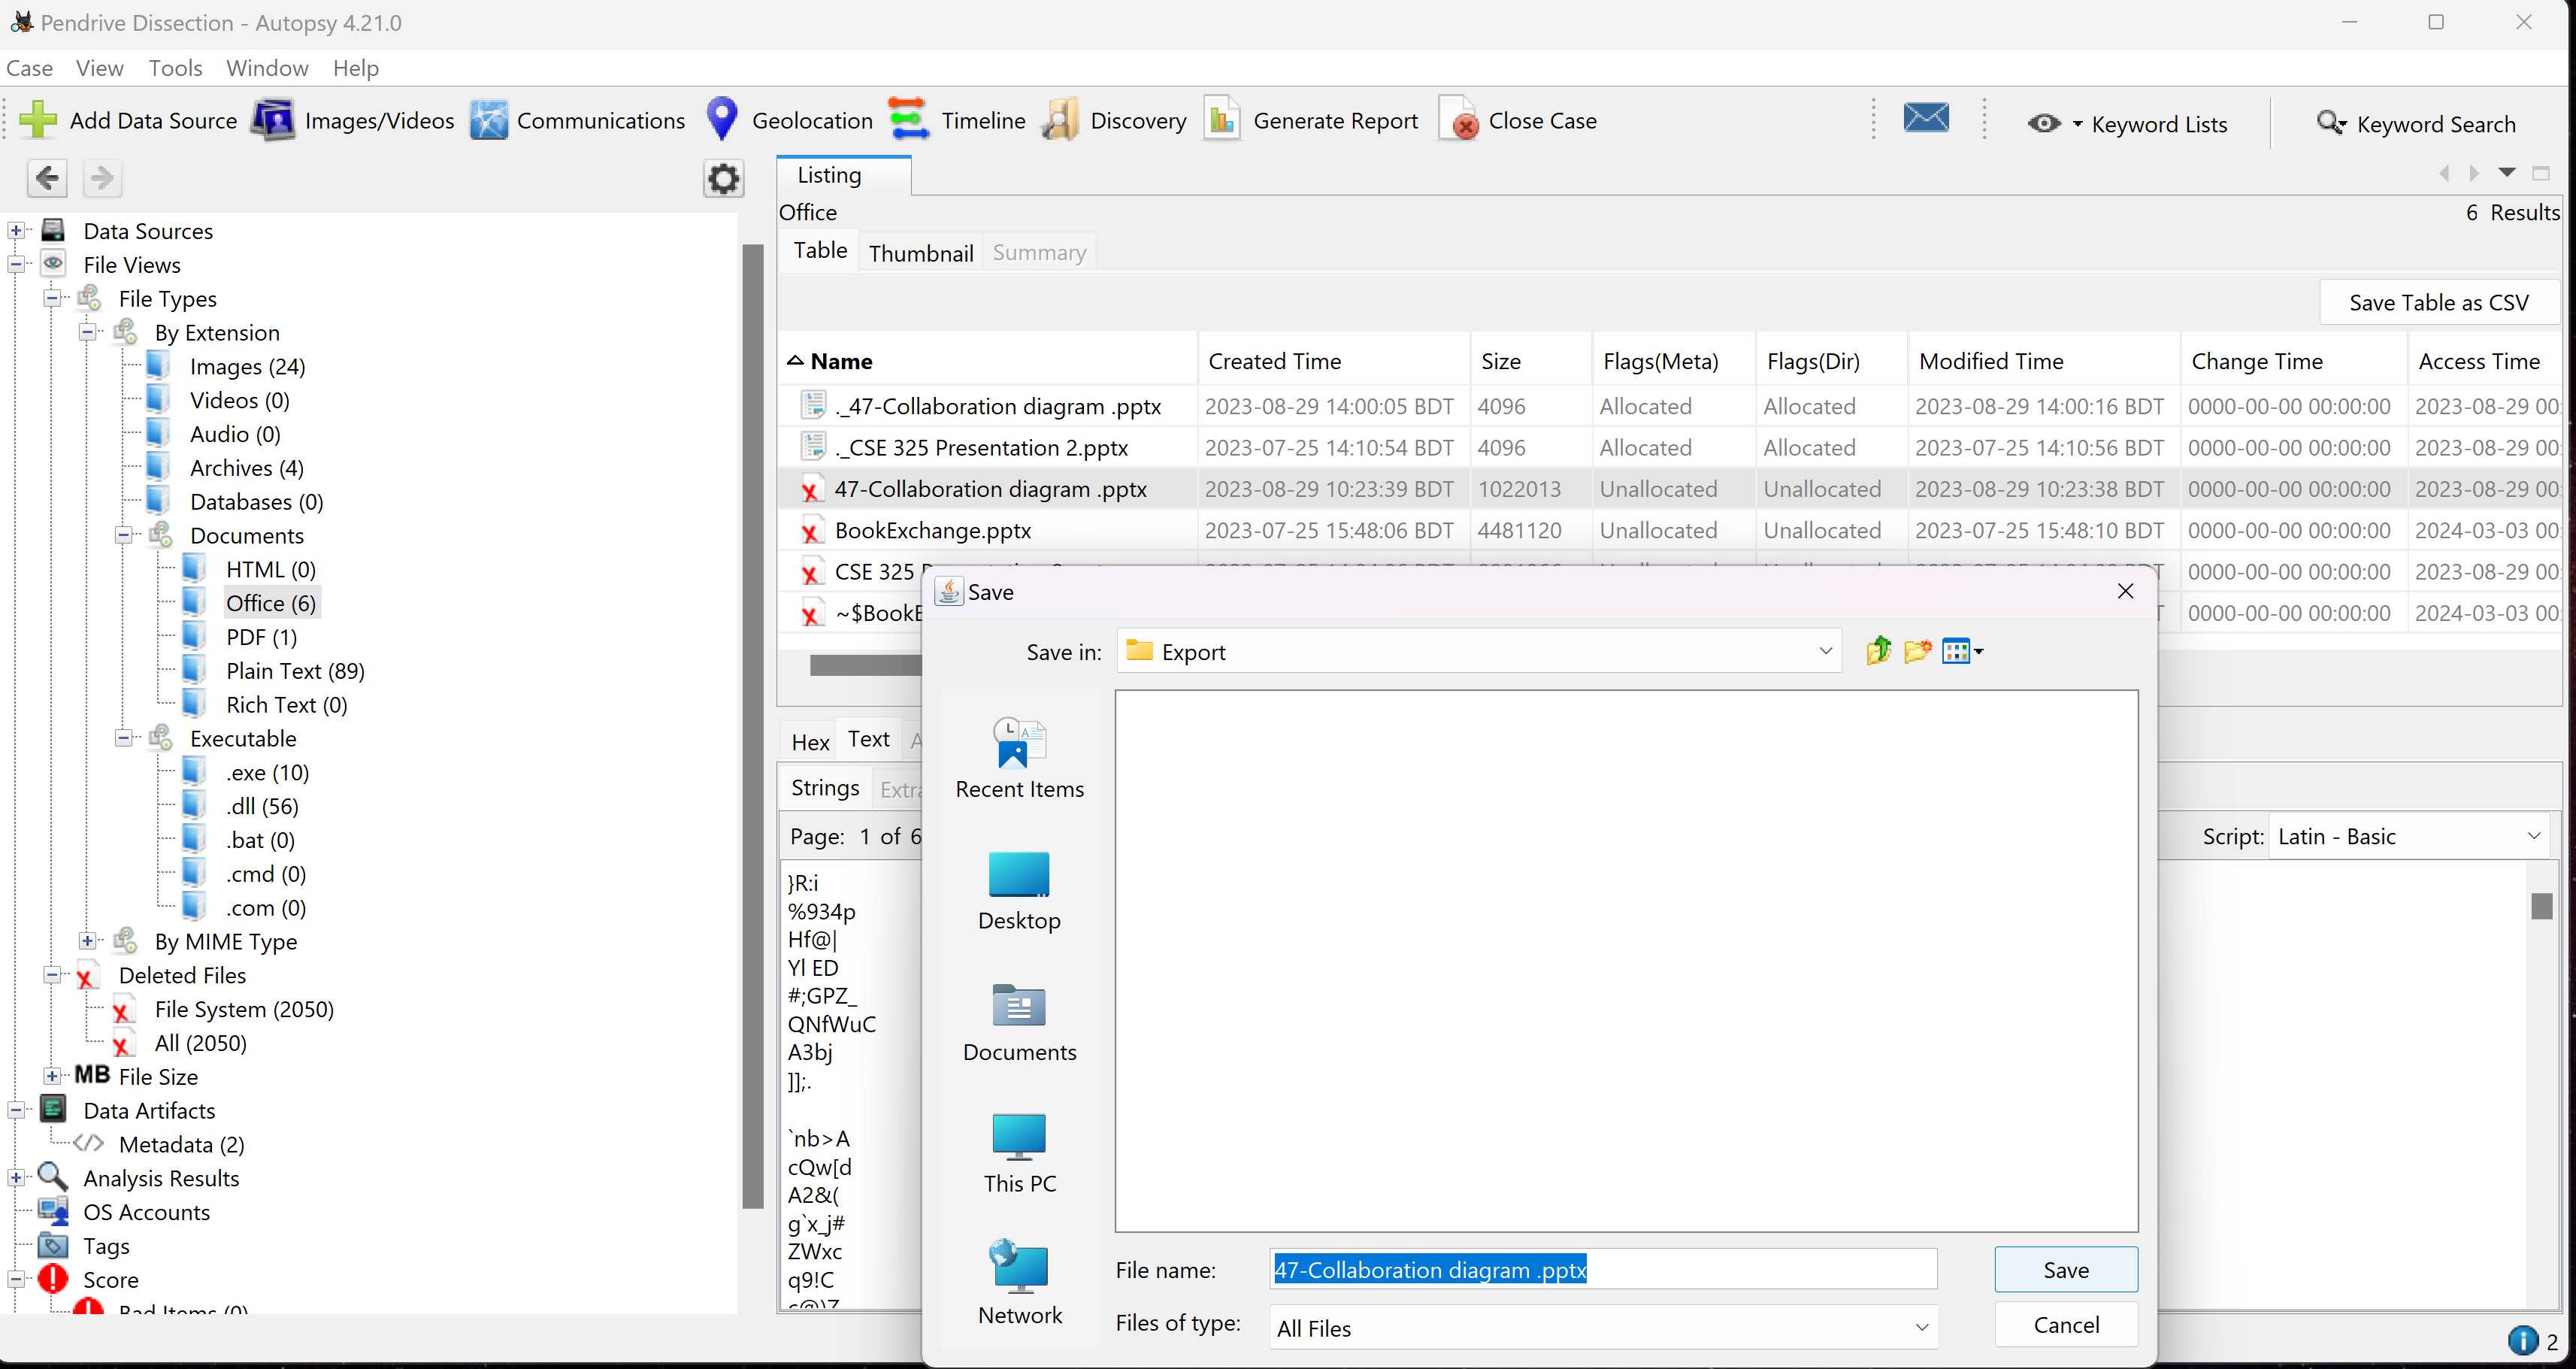
\includegraphics[width=0.75\textwidth]{4.3/Screenshot (417).png}
\end{center}

\begin{center}
    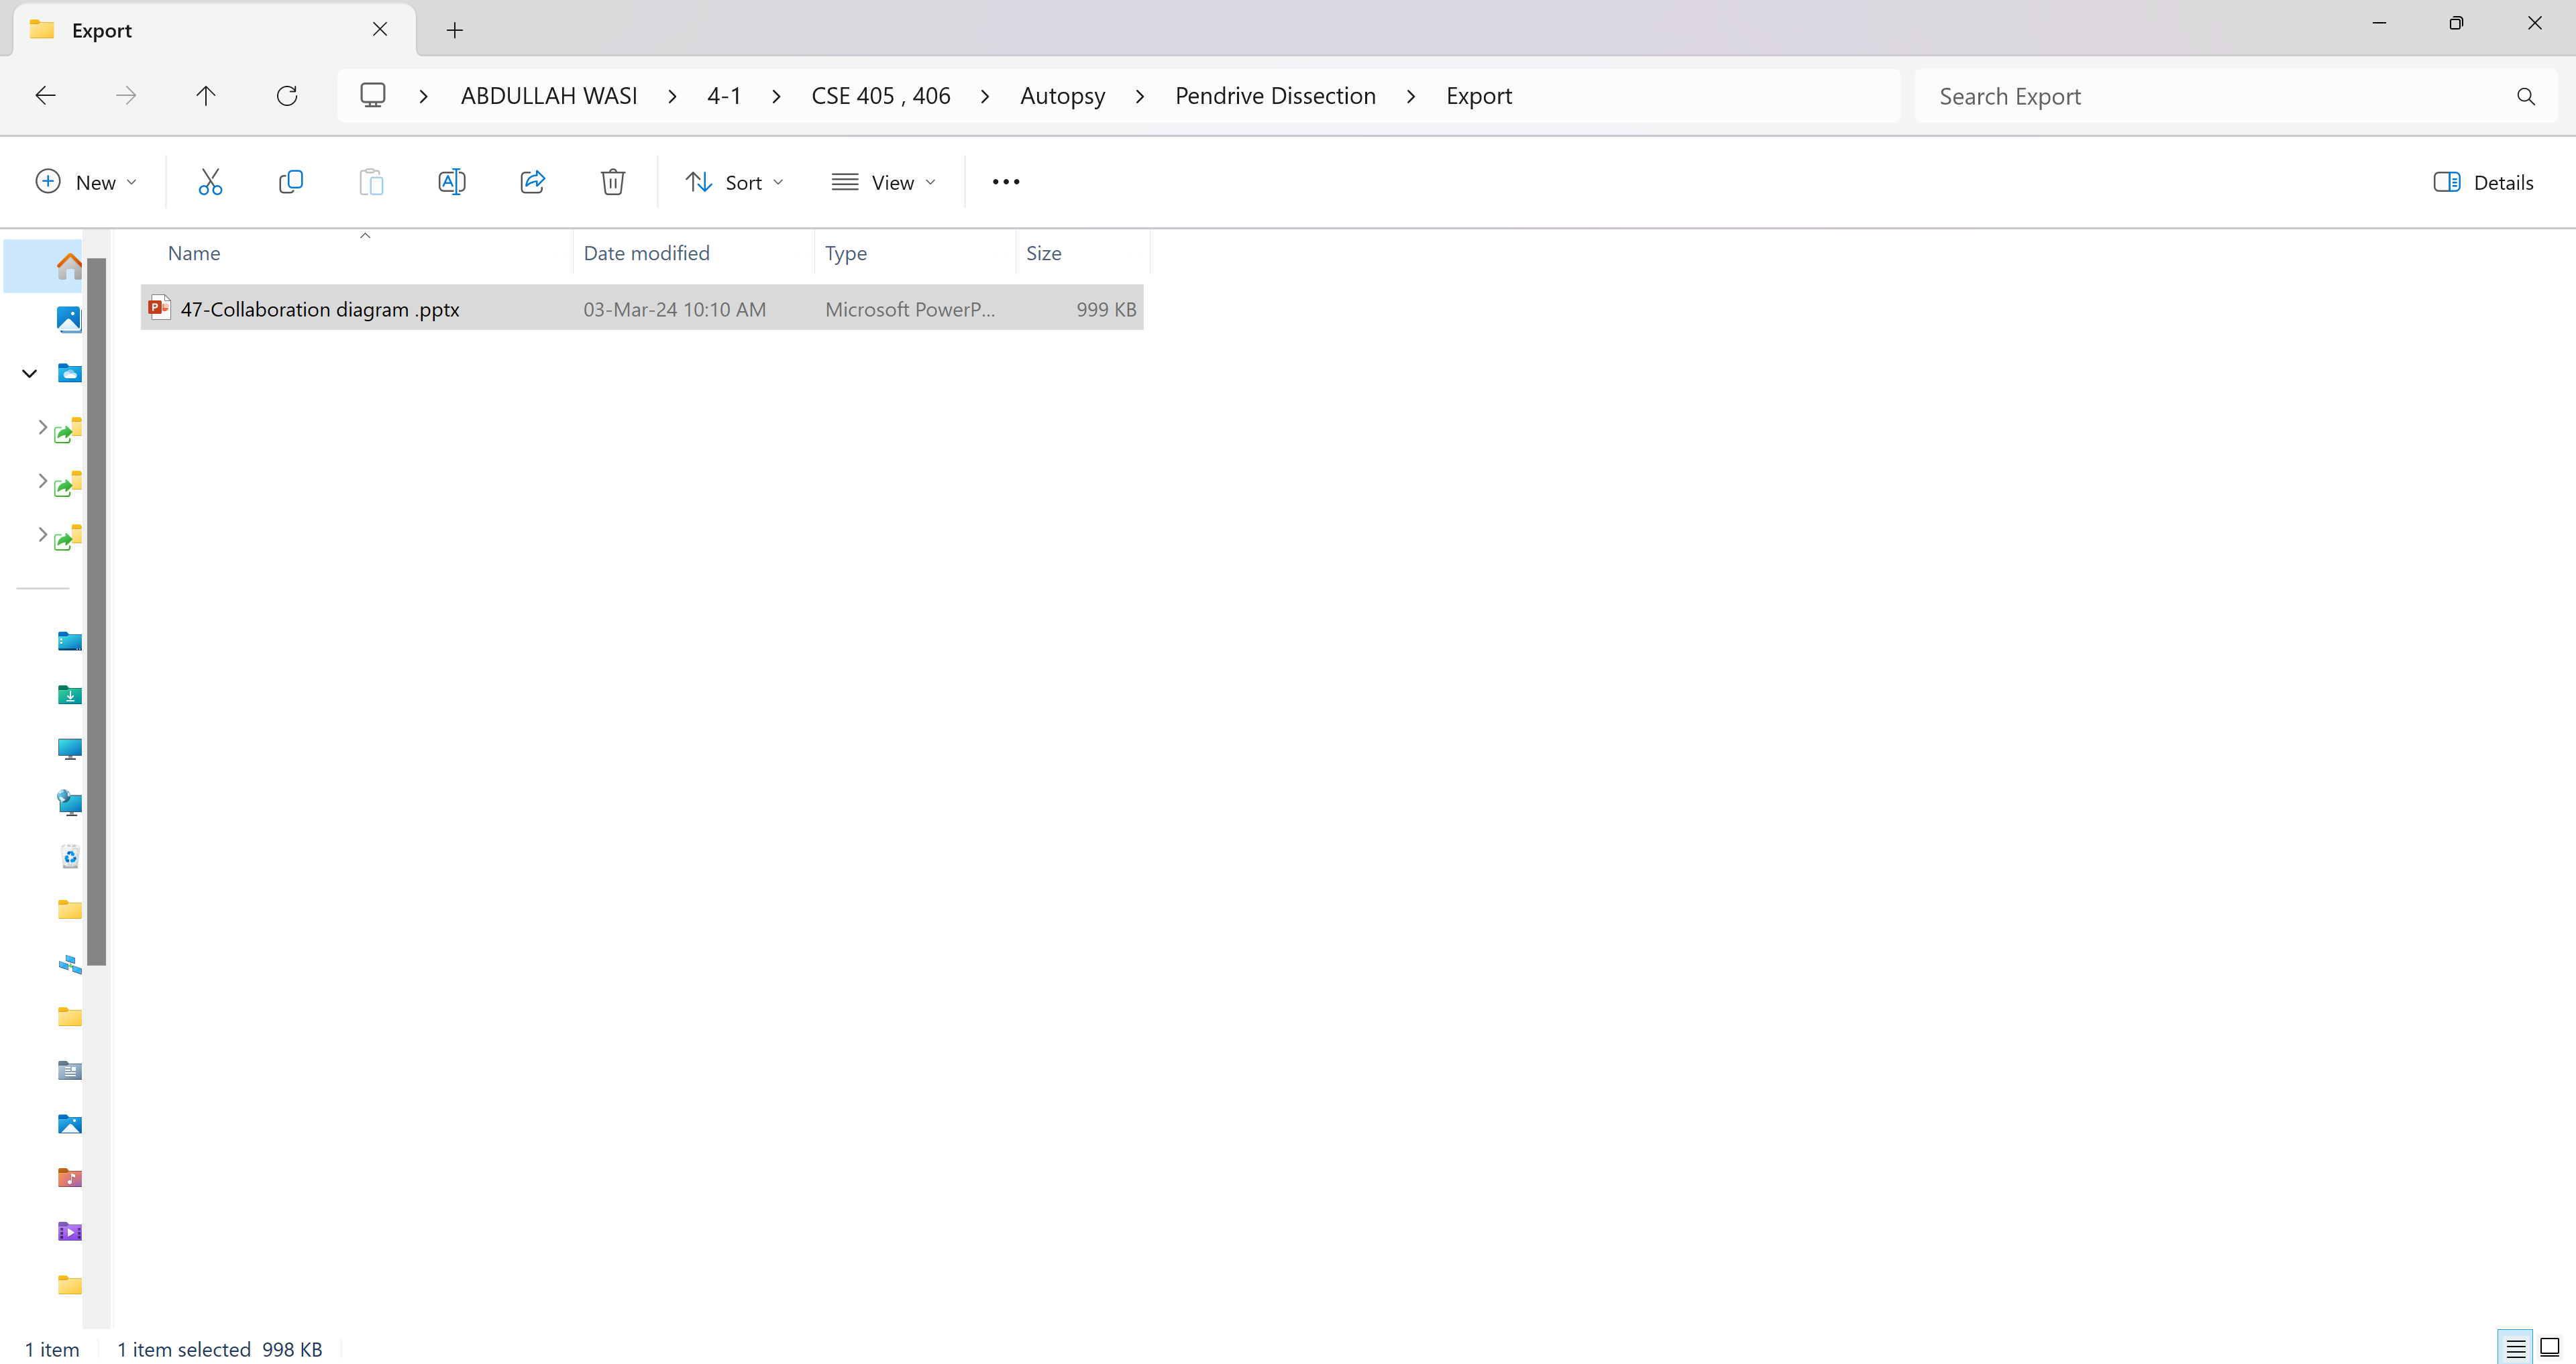
\includegraphics[width=0.75\textwidth]{4.3/Screenshot (418).png}
\end{center}

\section{Report Generation}
\subsection{Tagging Files}

When users discover something of interest, they can tag it by right-clicking on the item and selecting one of the tag options available:

If the file itself is noteworthy, users can choose the \textbf{TagFile} option. Alternatively, if the results of the analysis are significant, they can opt for the \textbf{TagResult} option.

\begin{center}
    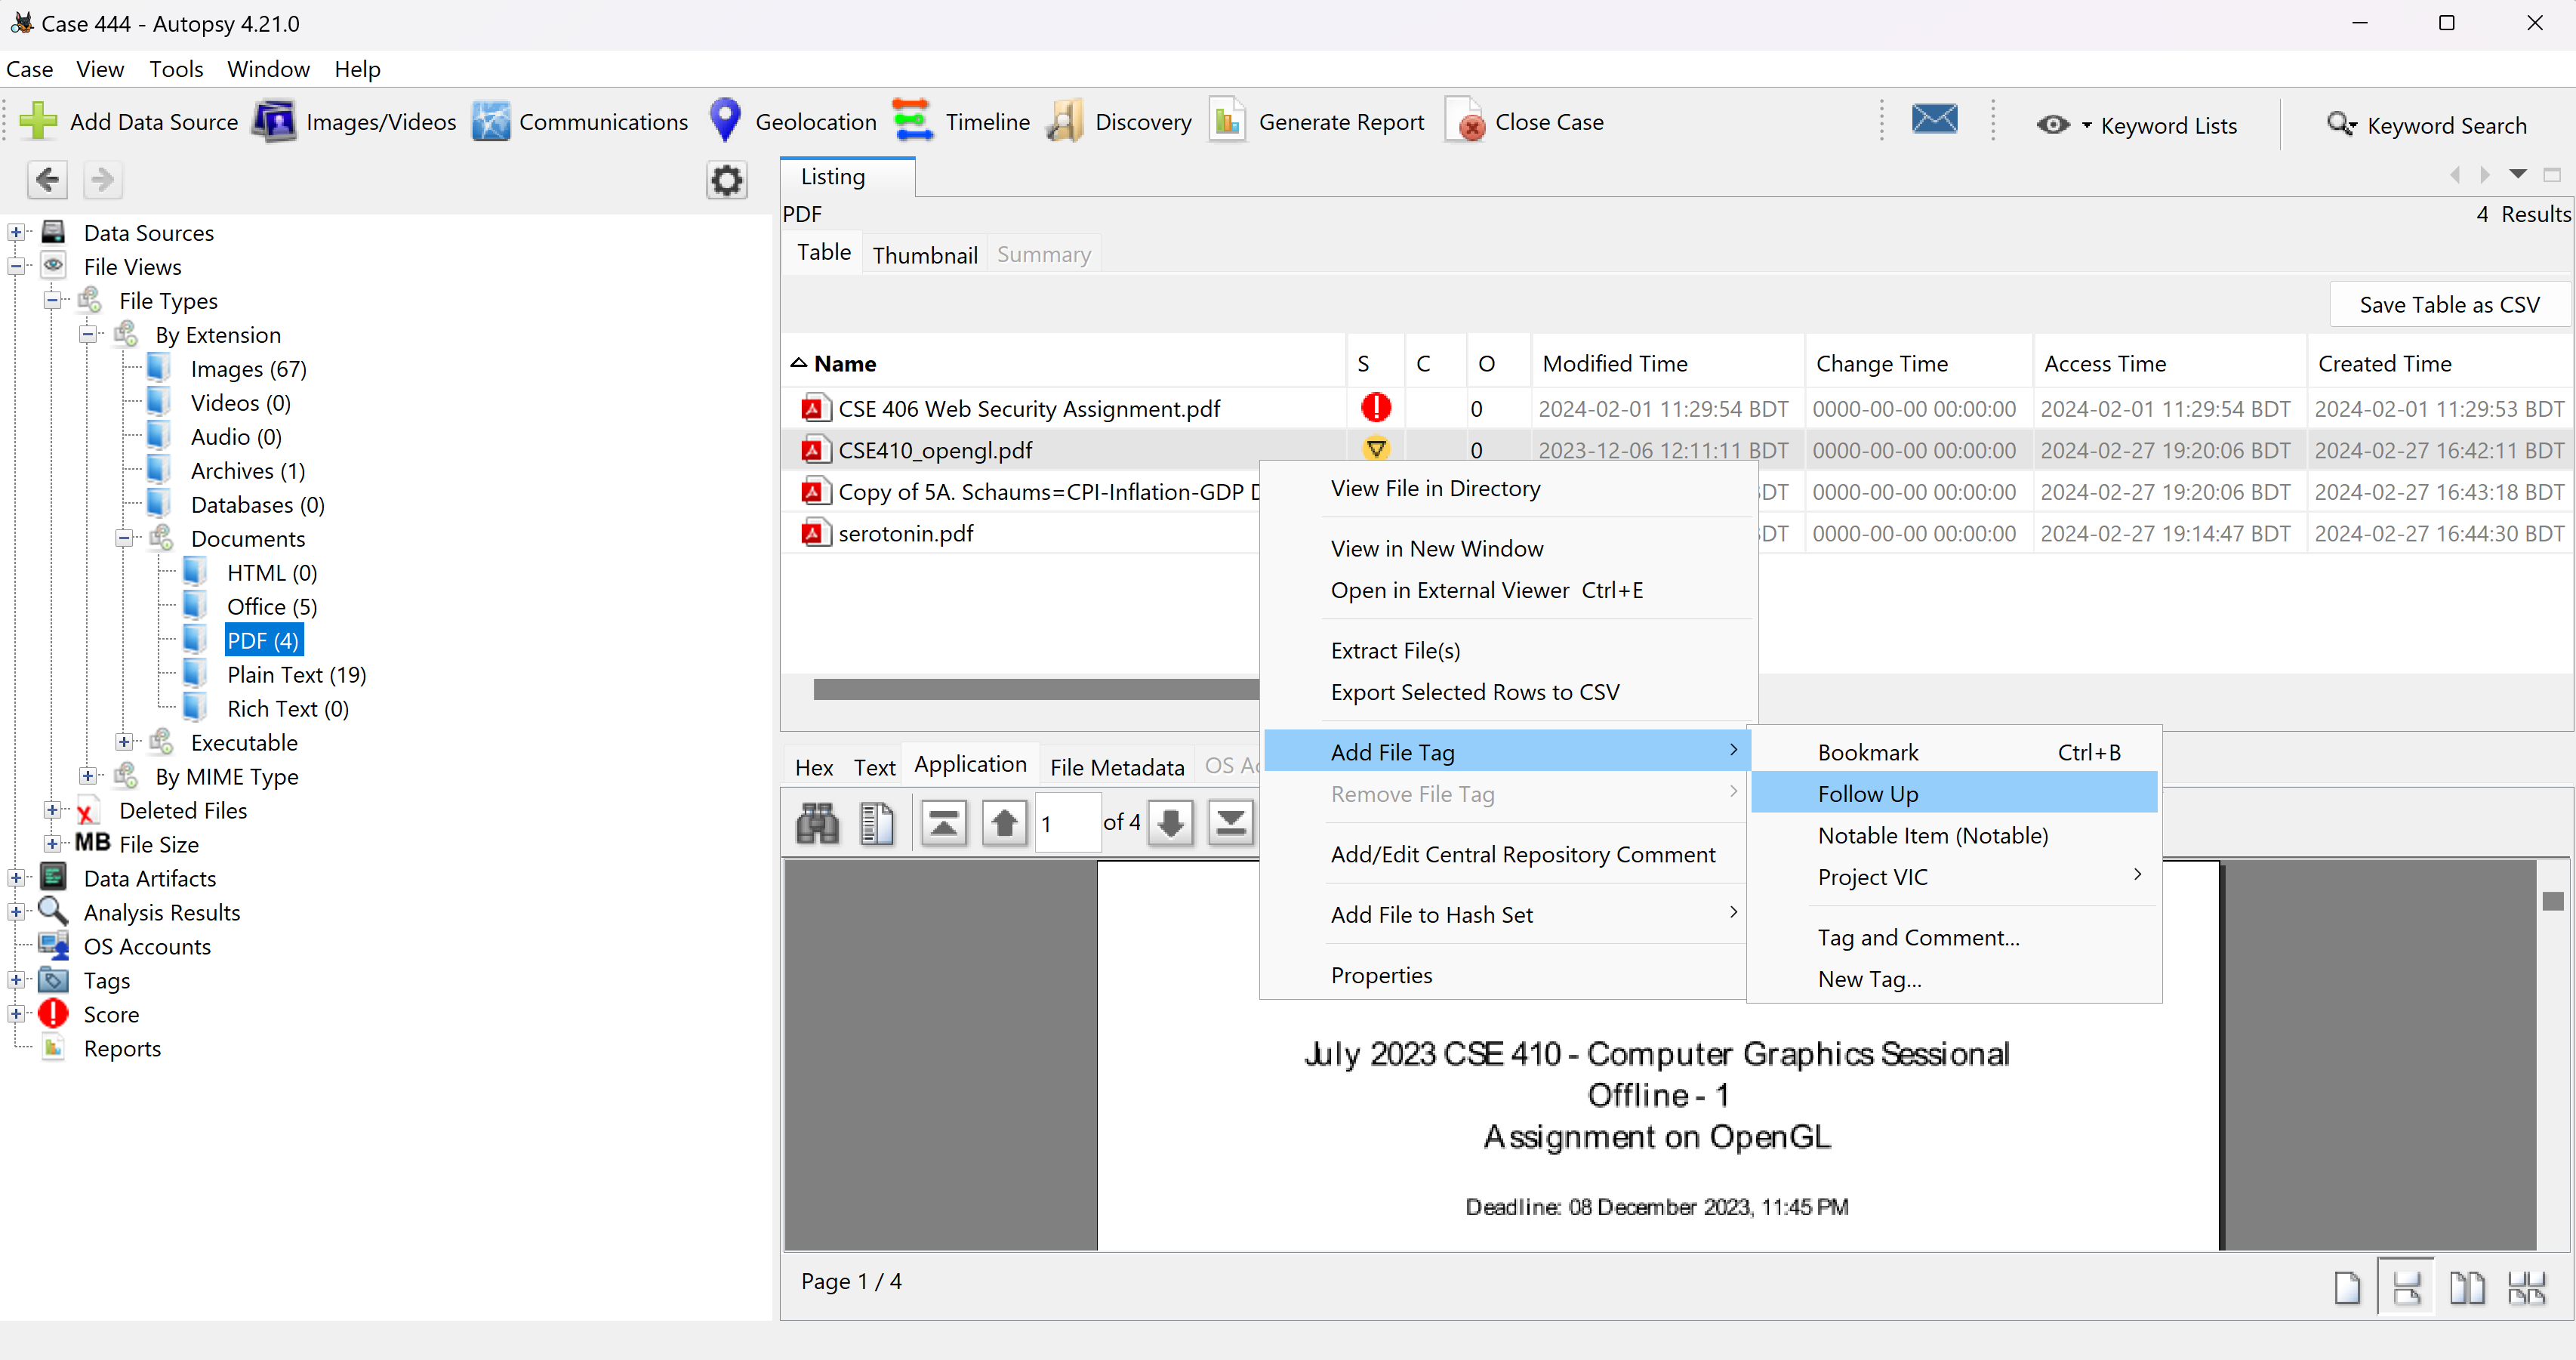
\includegraphics[width=0.75\textwidth]{5/5.1/Tagging.png}
\end{center}

\subsection{Tagging and Commenting}

Within Autopsy, commenting entails appending remarks and annotations to digital artifacts throughout a forensic examination. This supports documentation, collaboration, and context development among investigators, thus improving evidence organization and enhancing investigative insights and clarity. This functionality also allows for the application of multiple tags to a single file and aids in tracking the progress of the investigation.

\begin{center}
    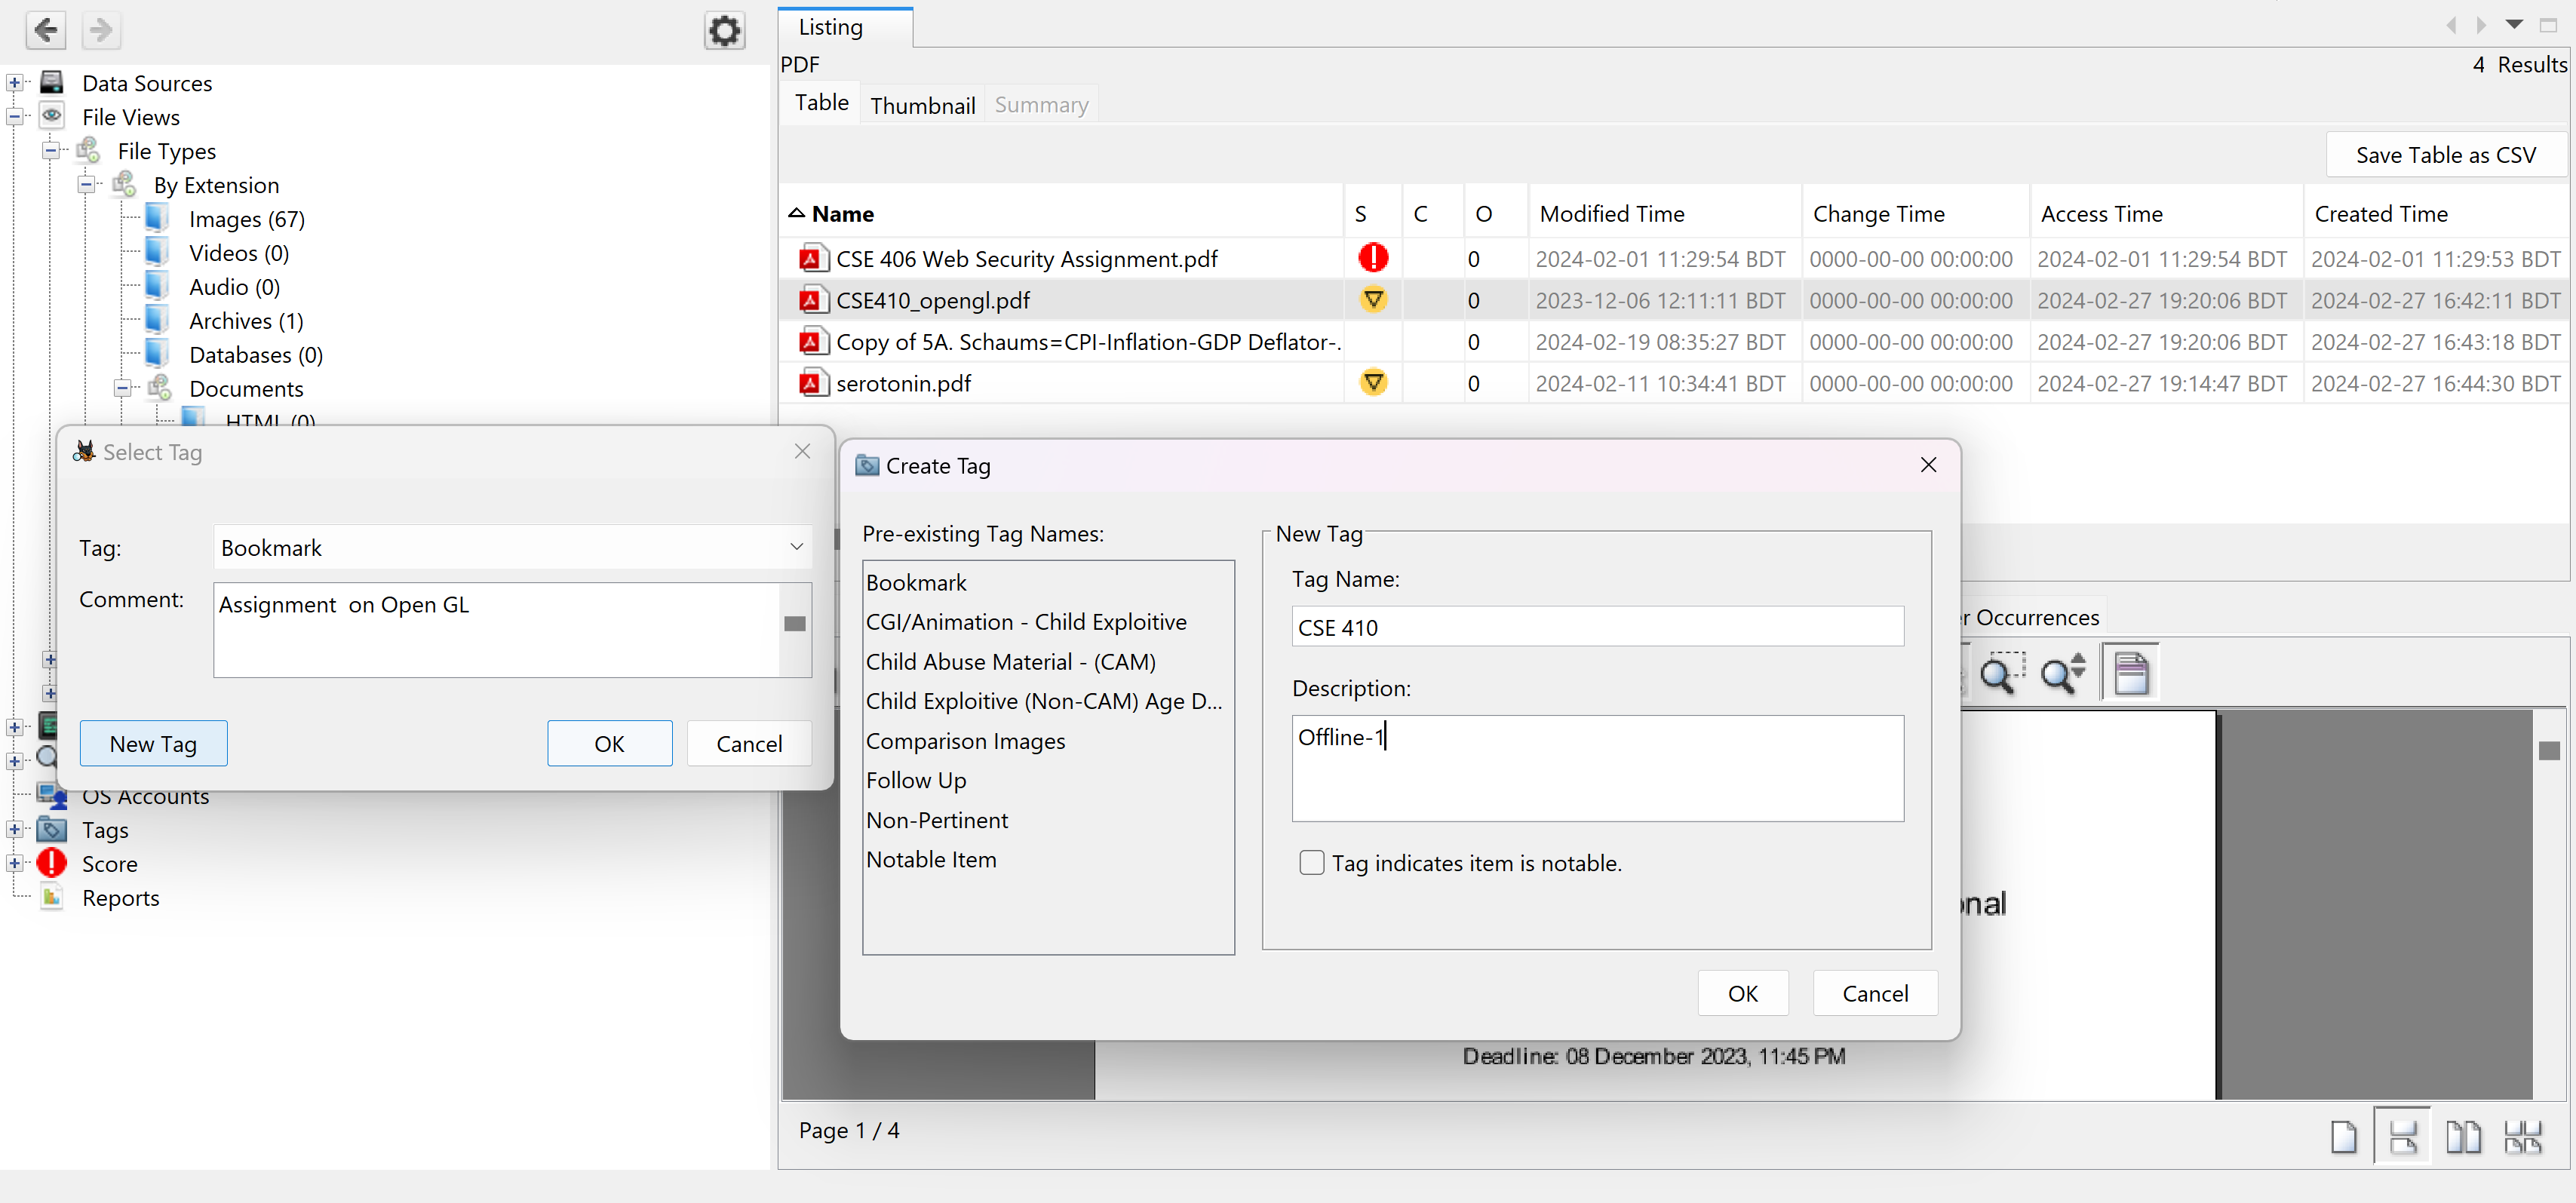
\includegraphics[width=0.75\textwidth]{5/5.2/Tagging & Commenting.png}
\end{center}

\subsection{Reporting}
The report modules enable users to extract crucial information from a case in diverse formats. This encompasses generating HTML or Excel reports containing all extracted content, keyword hits, and more from a case, as well as creating KML files from any coordinates discovered for integration into software such as Google Earth.

\begin{center}
    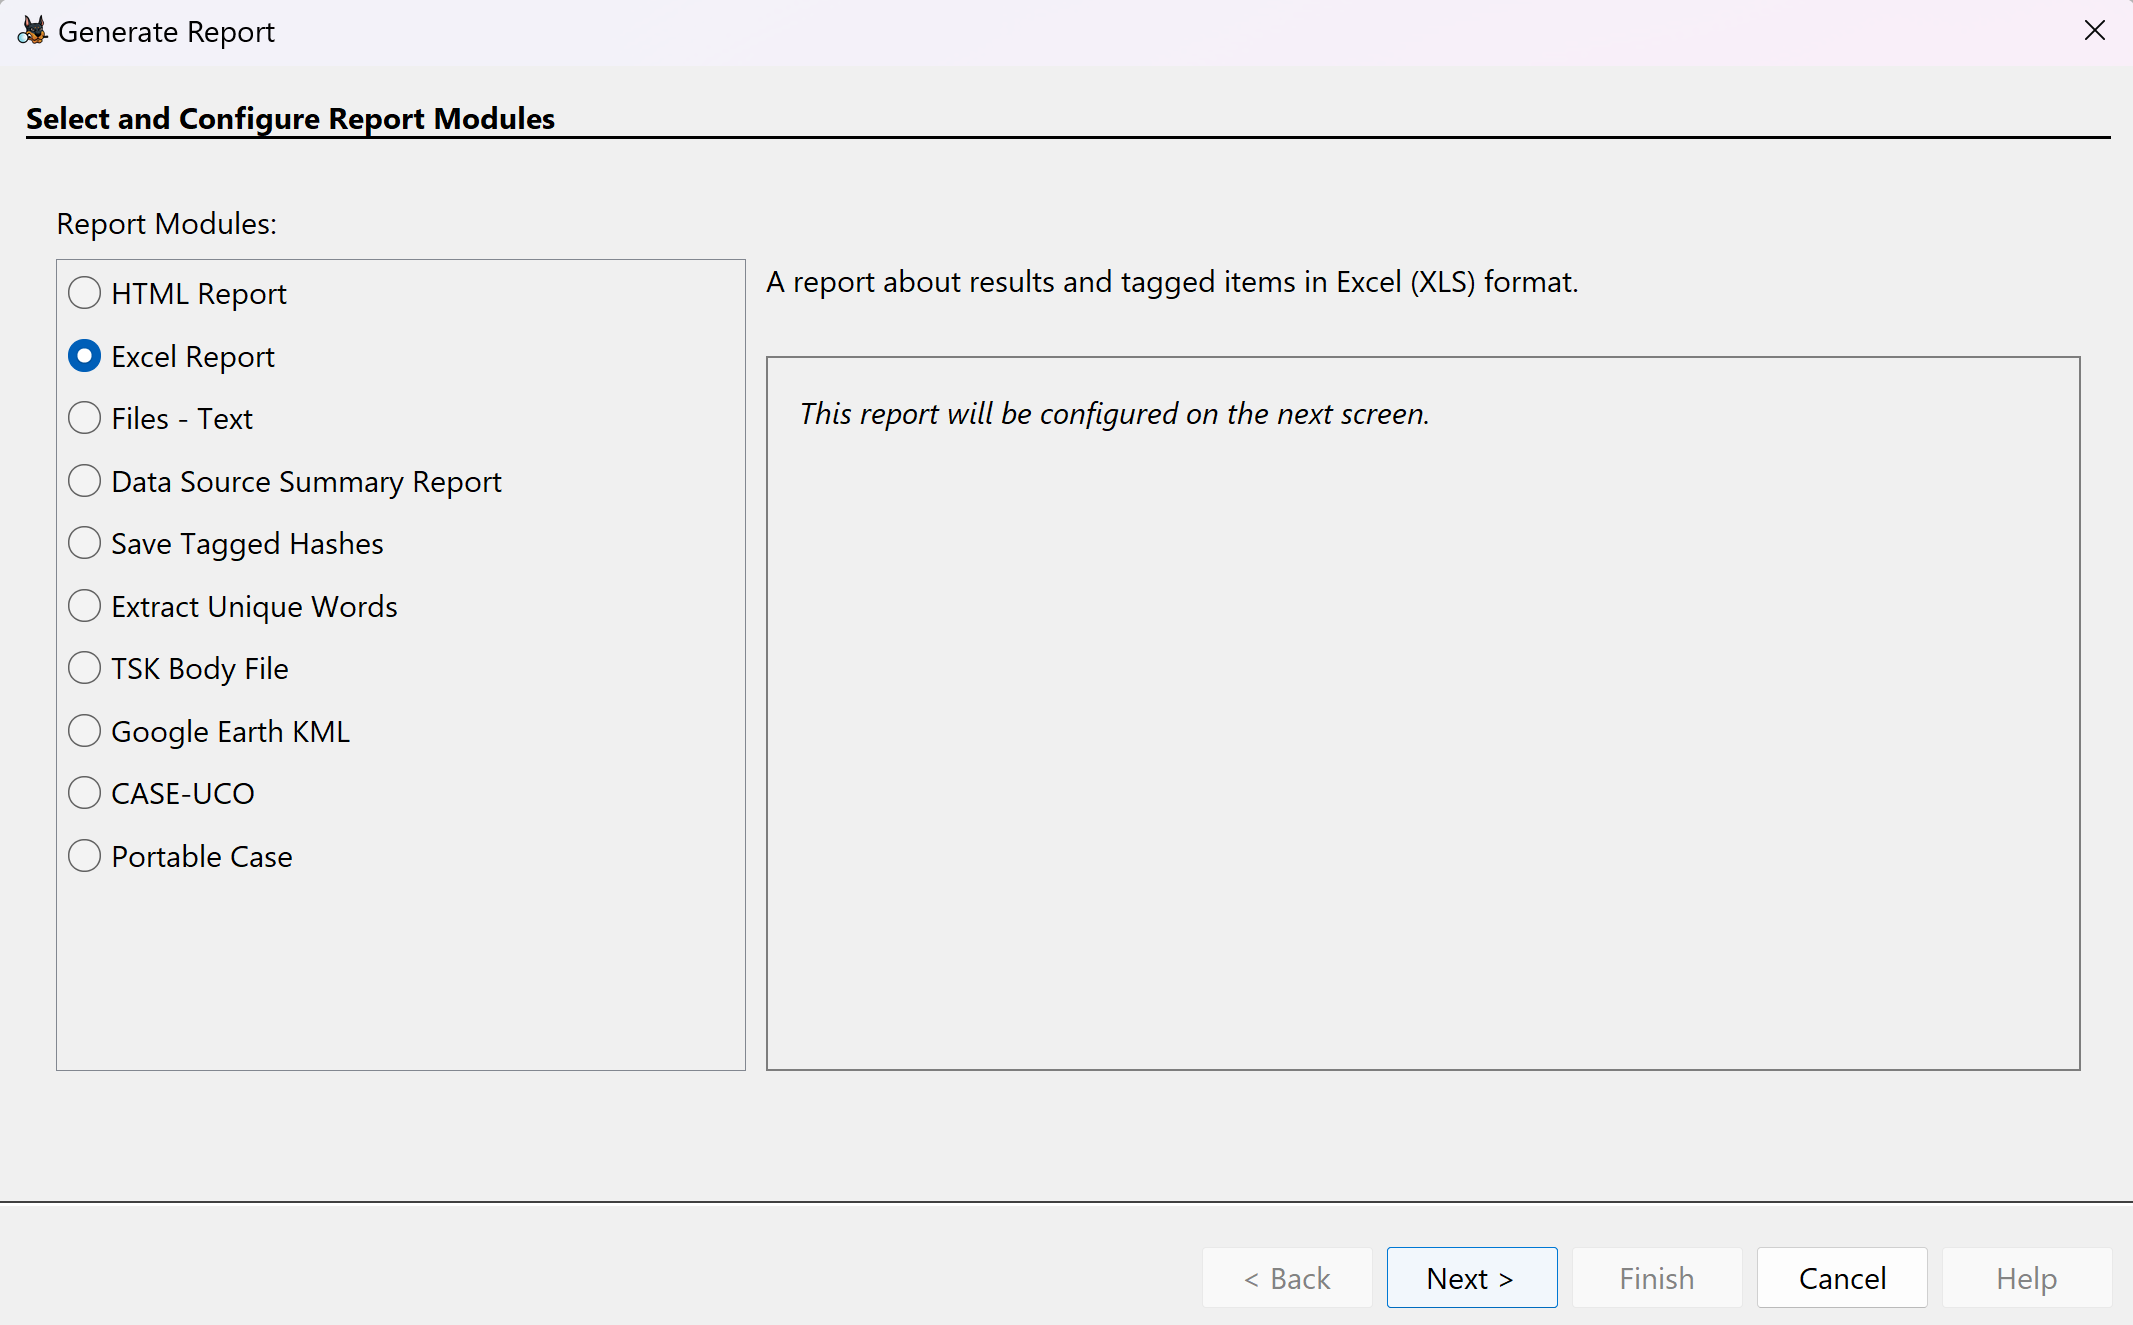
\includegraphics[width=0.75\textwidth]{5/5.3/Report Generation-1 .png}
\end{center}

Utilizing the tagged files, Autopsy has the capability to generate a report encompassing comprehensive information regarding the files. These reports can be generated in various formats and accessed through the \textbf{Reports} tab.

\begin{center}
    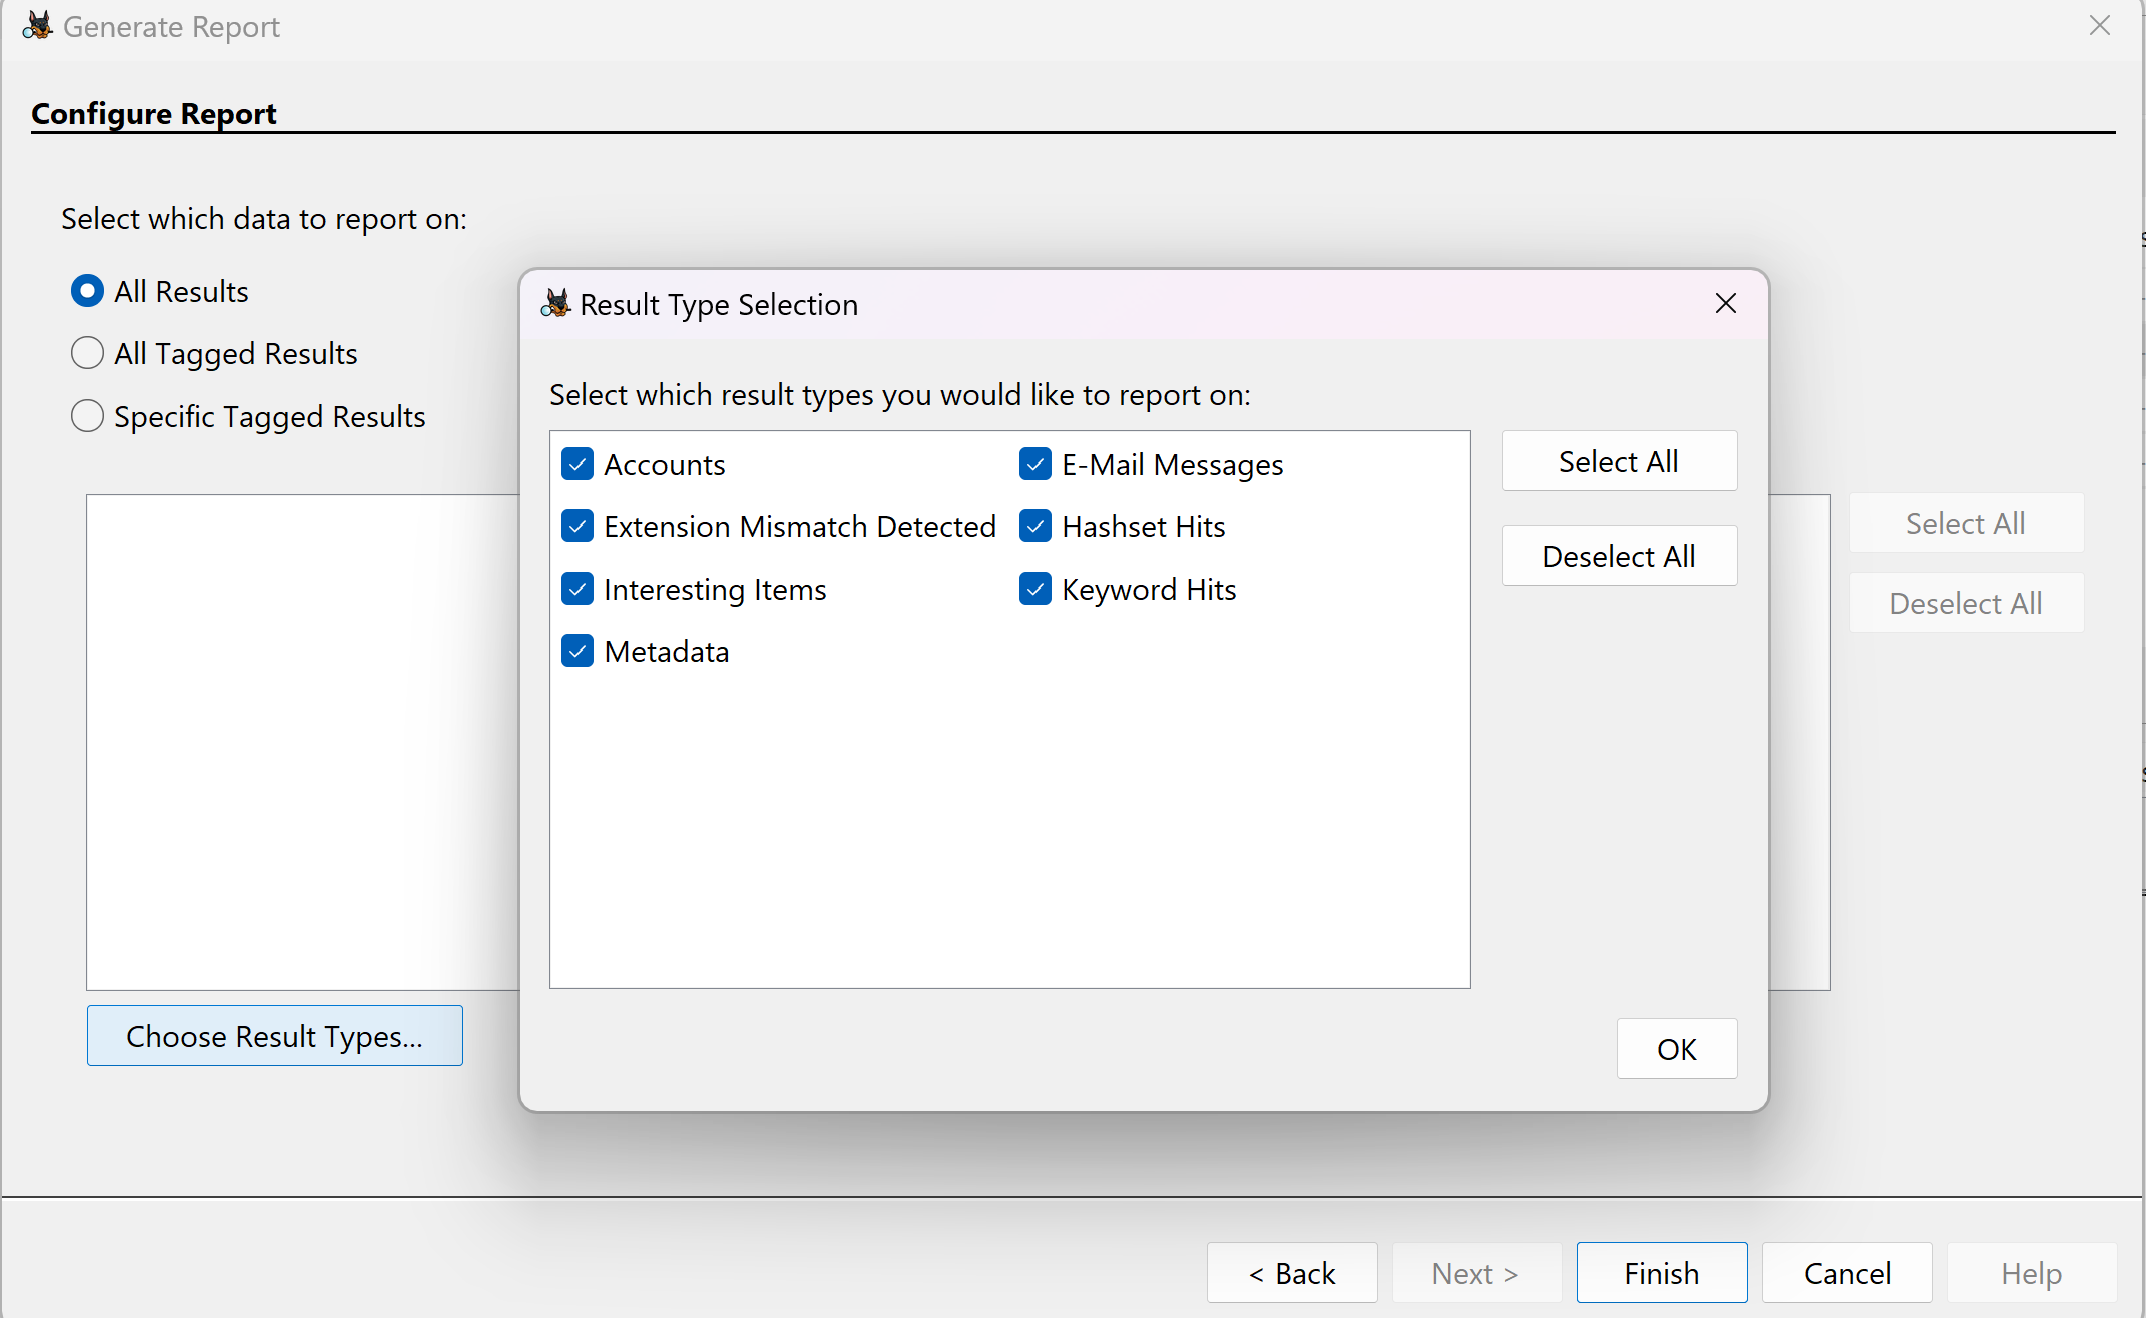
\includegraphics[width=0.75\textwidth]{5/5.3/Report Generation-2 .png}
\end{center}
and generated report is 
\begin{center}
    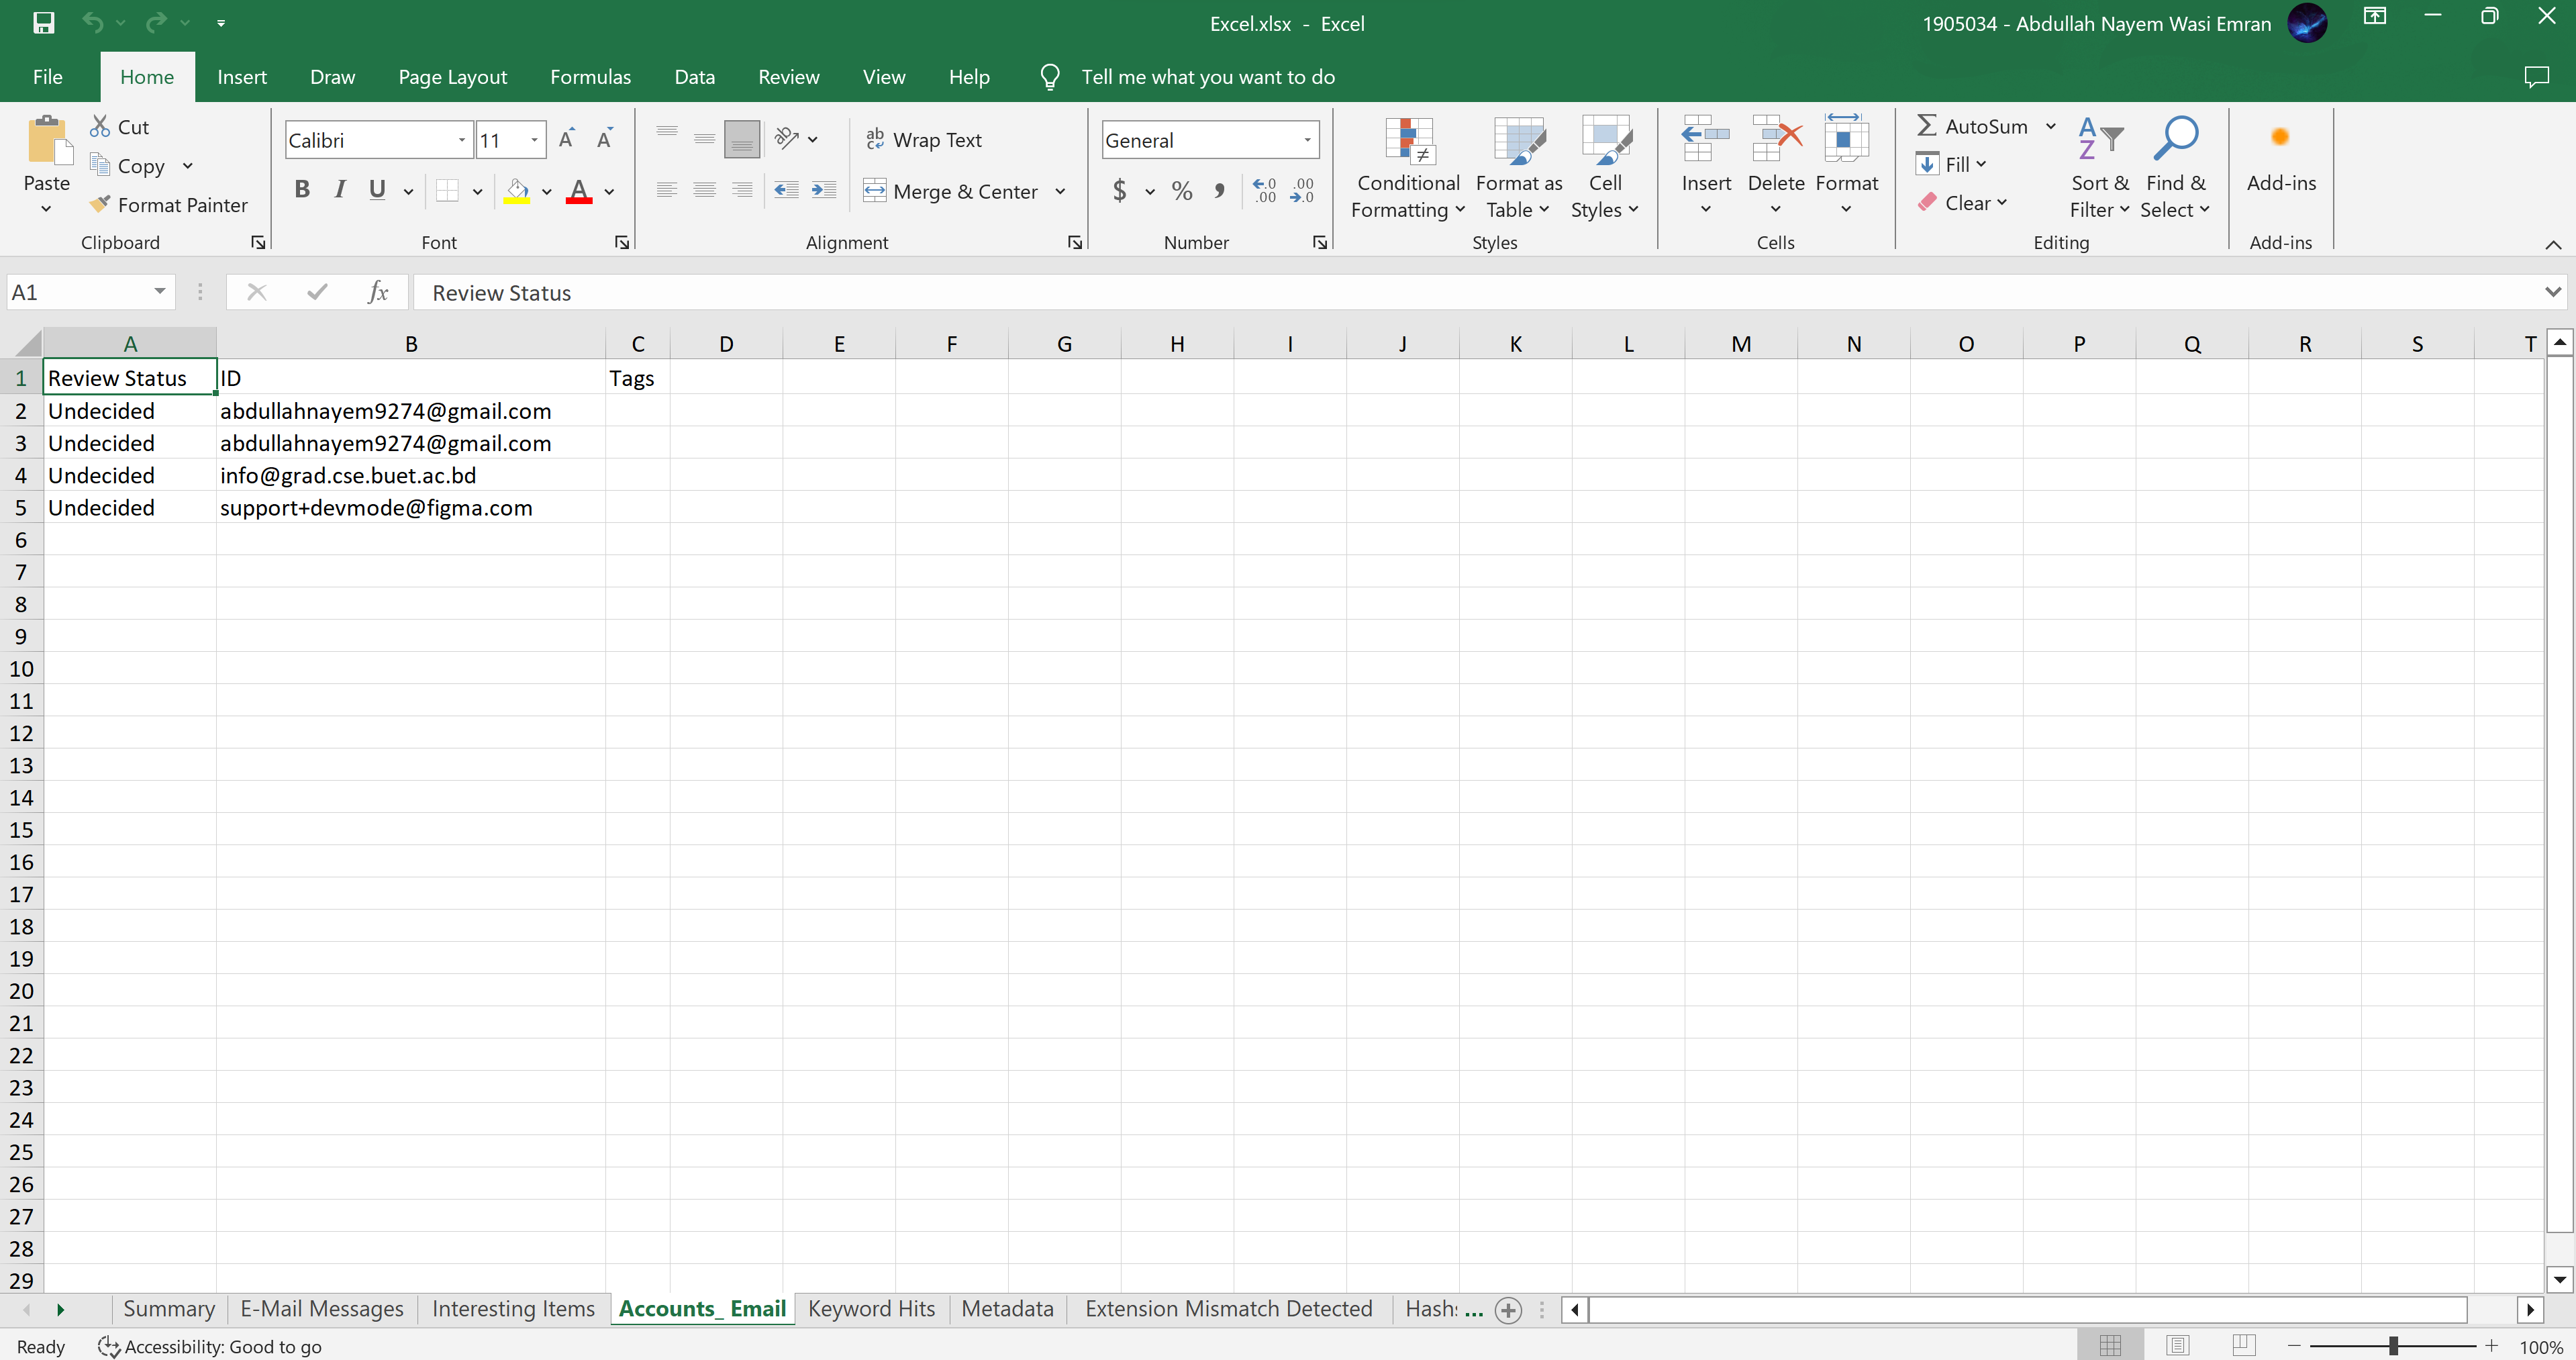
\includegraphics[width=0.75\textwidth]{5/5.3/Report Generation-3.png}
\end{center}

\section{Autopsy Functionality Testing}
\subsection{Extended DOS Partition Test}
\subsubsection*{Introduction}
Many DOS partition utilities typically restrict users from creating a third entry within an extended partition. To investigate this limitation, an experiment involved manually altering the partition table using a hex editor to create a third entry. Subsequently, the system was booted, and both Windows and Linux successfully detected and permitted mounting of the third entry within the extended partition. This validation aimed to ensure that forensic tools, like Autopsy, also facilitate investigators in examining partitions within the third entry of an extended partition.

\subsubsection*{Source}
The disk image can be downloaded from here: \href{http://prdownloads.sourceforge.net/dftt/1-extend-part.zip?download}{Disk Image Download Link}

\subsubsection*{Outputs from Autopsy}
\begin{center}
    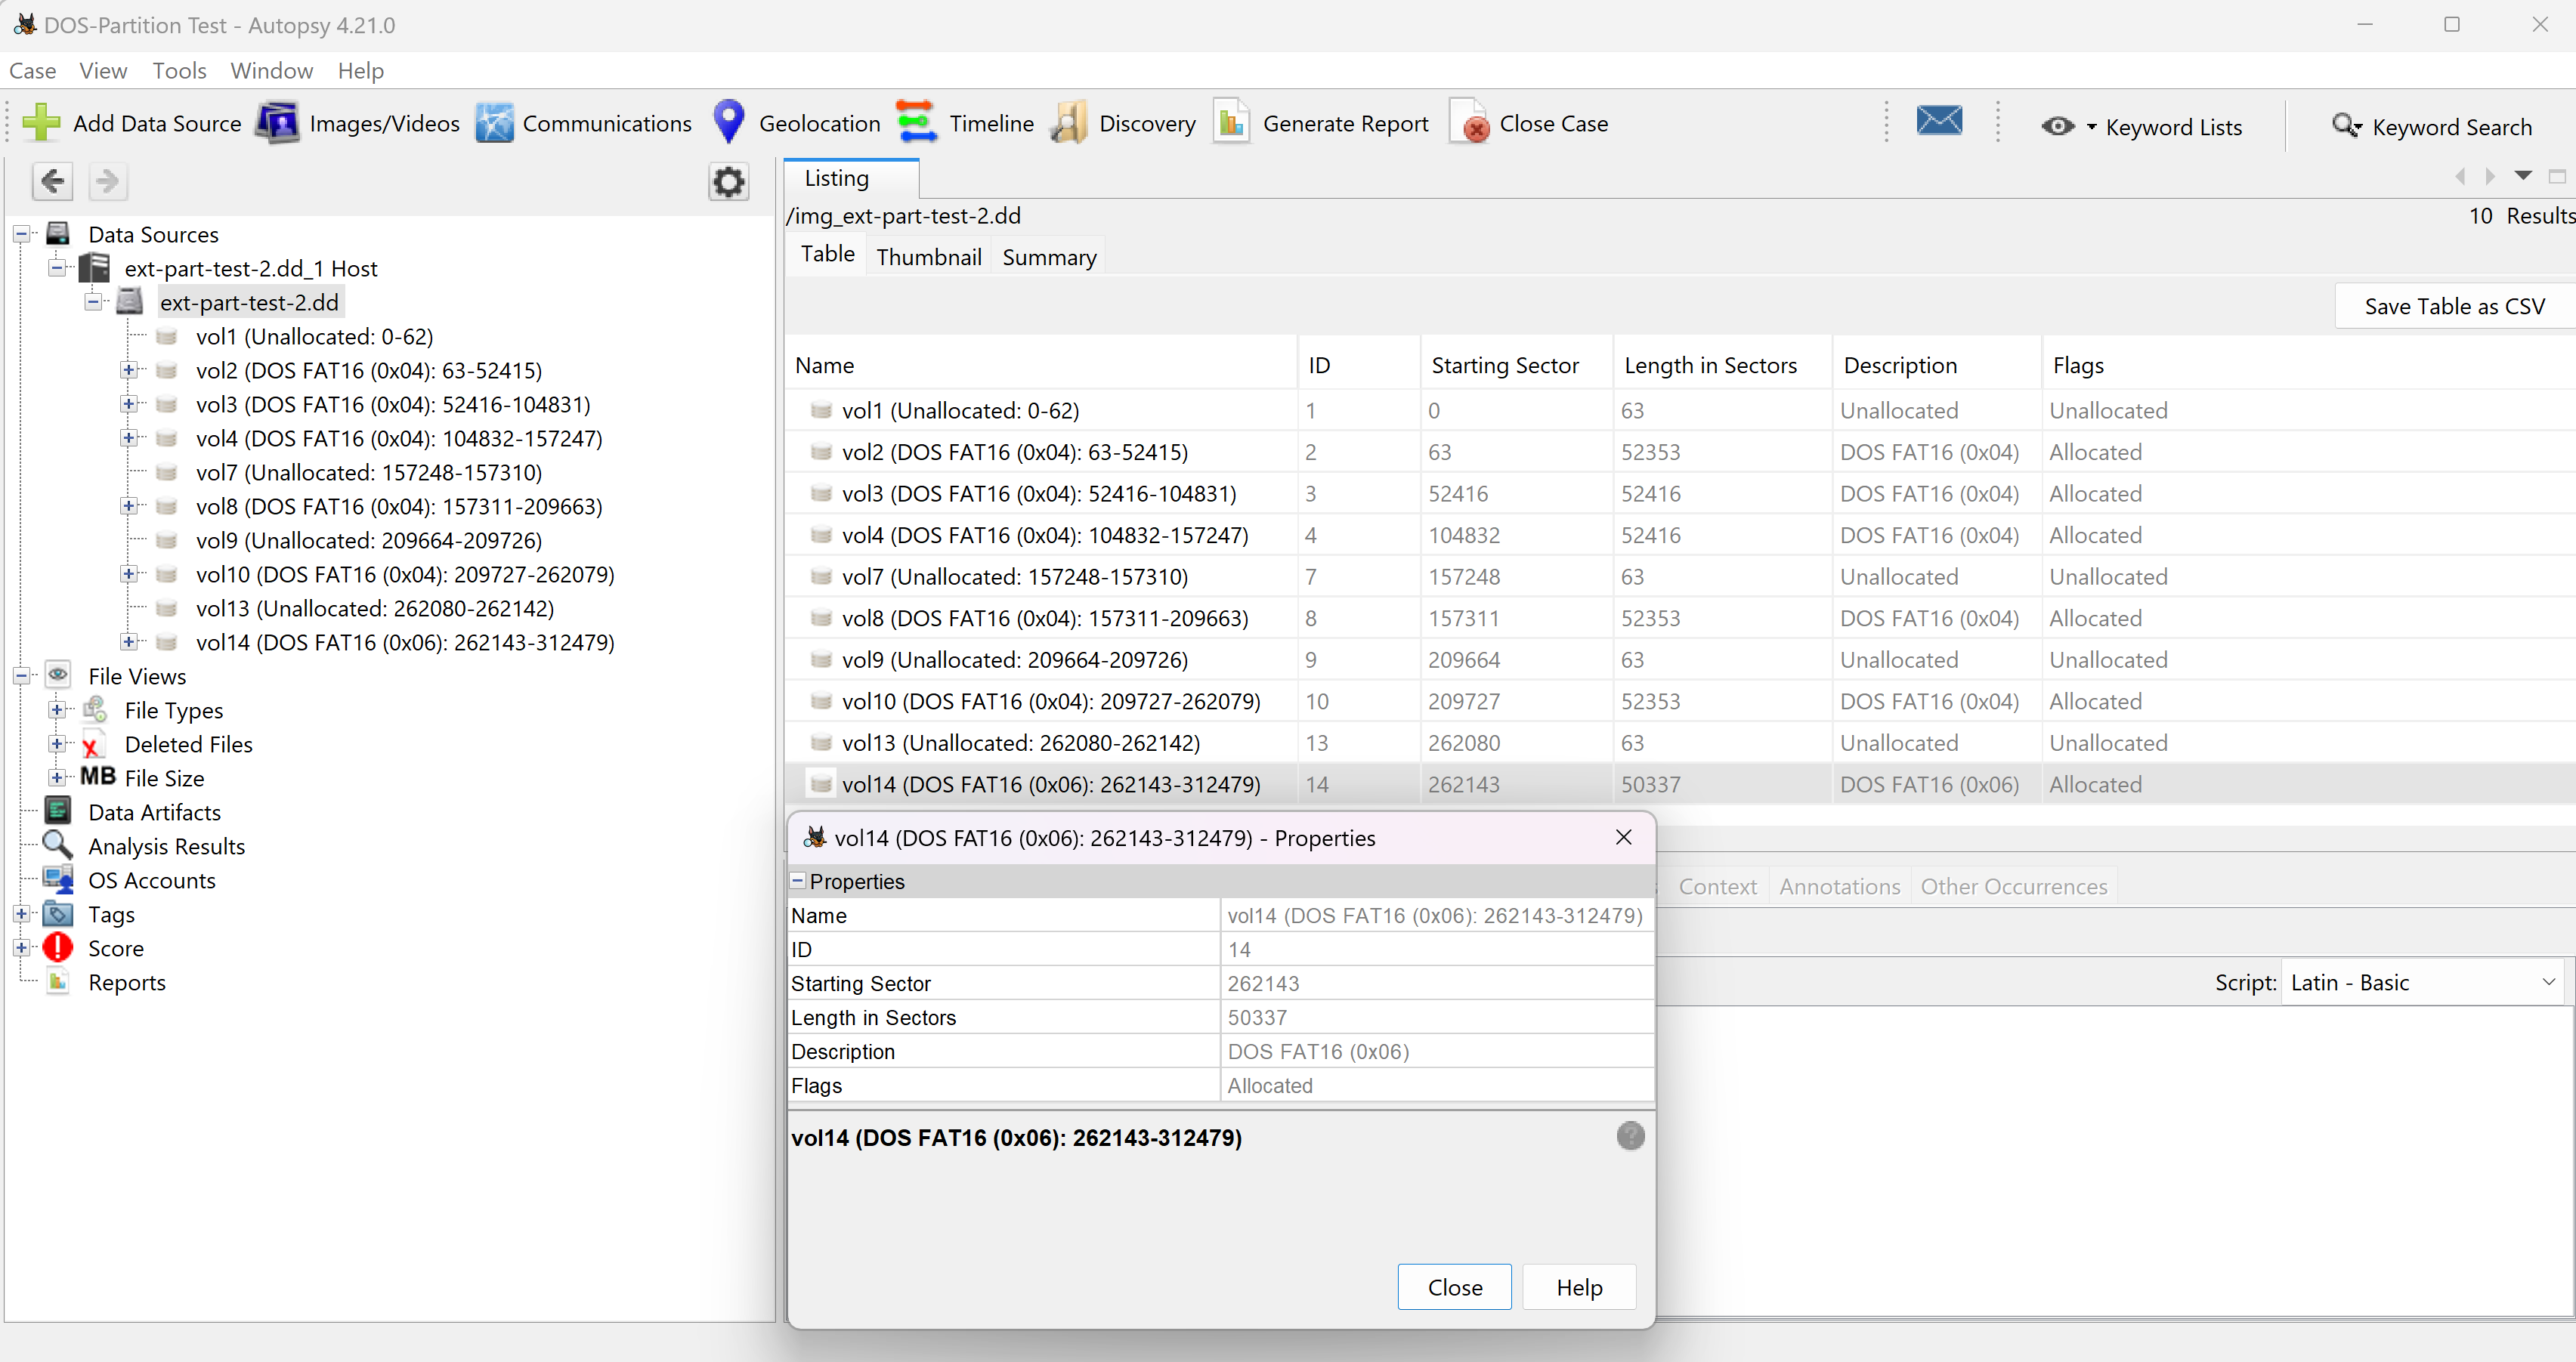
\includegraphics[width=0.75\textwidth]{6/6.1/Extended DOS Partition.png}
\end{center}

\subsubsection*{Conclusion}
\begin{itemize}
    \item Autopsy accurately identifies and displays partitions within a disk image.
    \item Autopsy correctly identifies and displays extended partitions (logical partitions) within primary extended partitions.
    \item Autopsy can present files and their properties within partitions, even if the file is empty.
\end{itemize}

\subsection{FAT Keyword Search}
\subsubsection*{Introduction}
The provided test image comprises a \textbf{FAT file system} containing numerous ASCII strings. The objective of this examination is to determine which tools are capable of identifying various types of strings. Thus, it's important to note that not all strings listed in the table below will necessarily be detected by each tool. Failure to detect a specific string does not necessarily indicate an error in the tool. For instance, the string '1slack1' may extend beyond the end of a file and into its slack space, which may or may not be detected by different tools. As long as the functionality of the tool is adequately documented, it is the responsibility of the user to employ the tool appropriately to collect potential evidence.

\subsubsection*{Source}
The disk image can be downloaded from here: \href{http://prdownloads.sourceforge.net/dftt/2-kwsrch-fat.zip?download}{Disk Image Download Link}

\subsubsection*{Outputs from Autopsy}
\begin{center}
    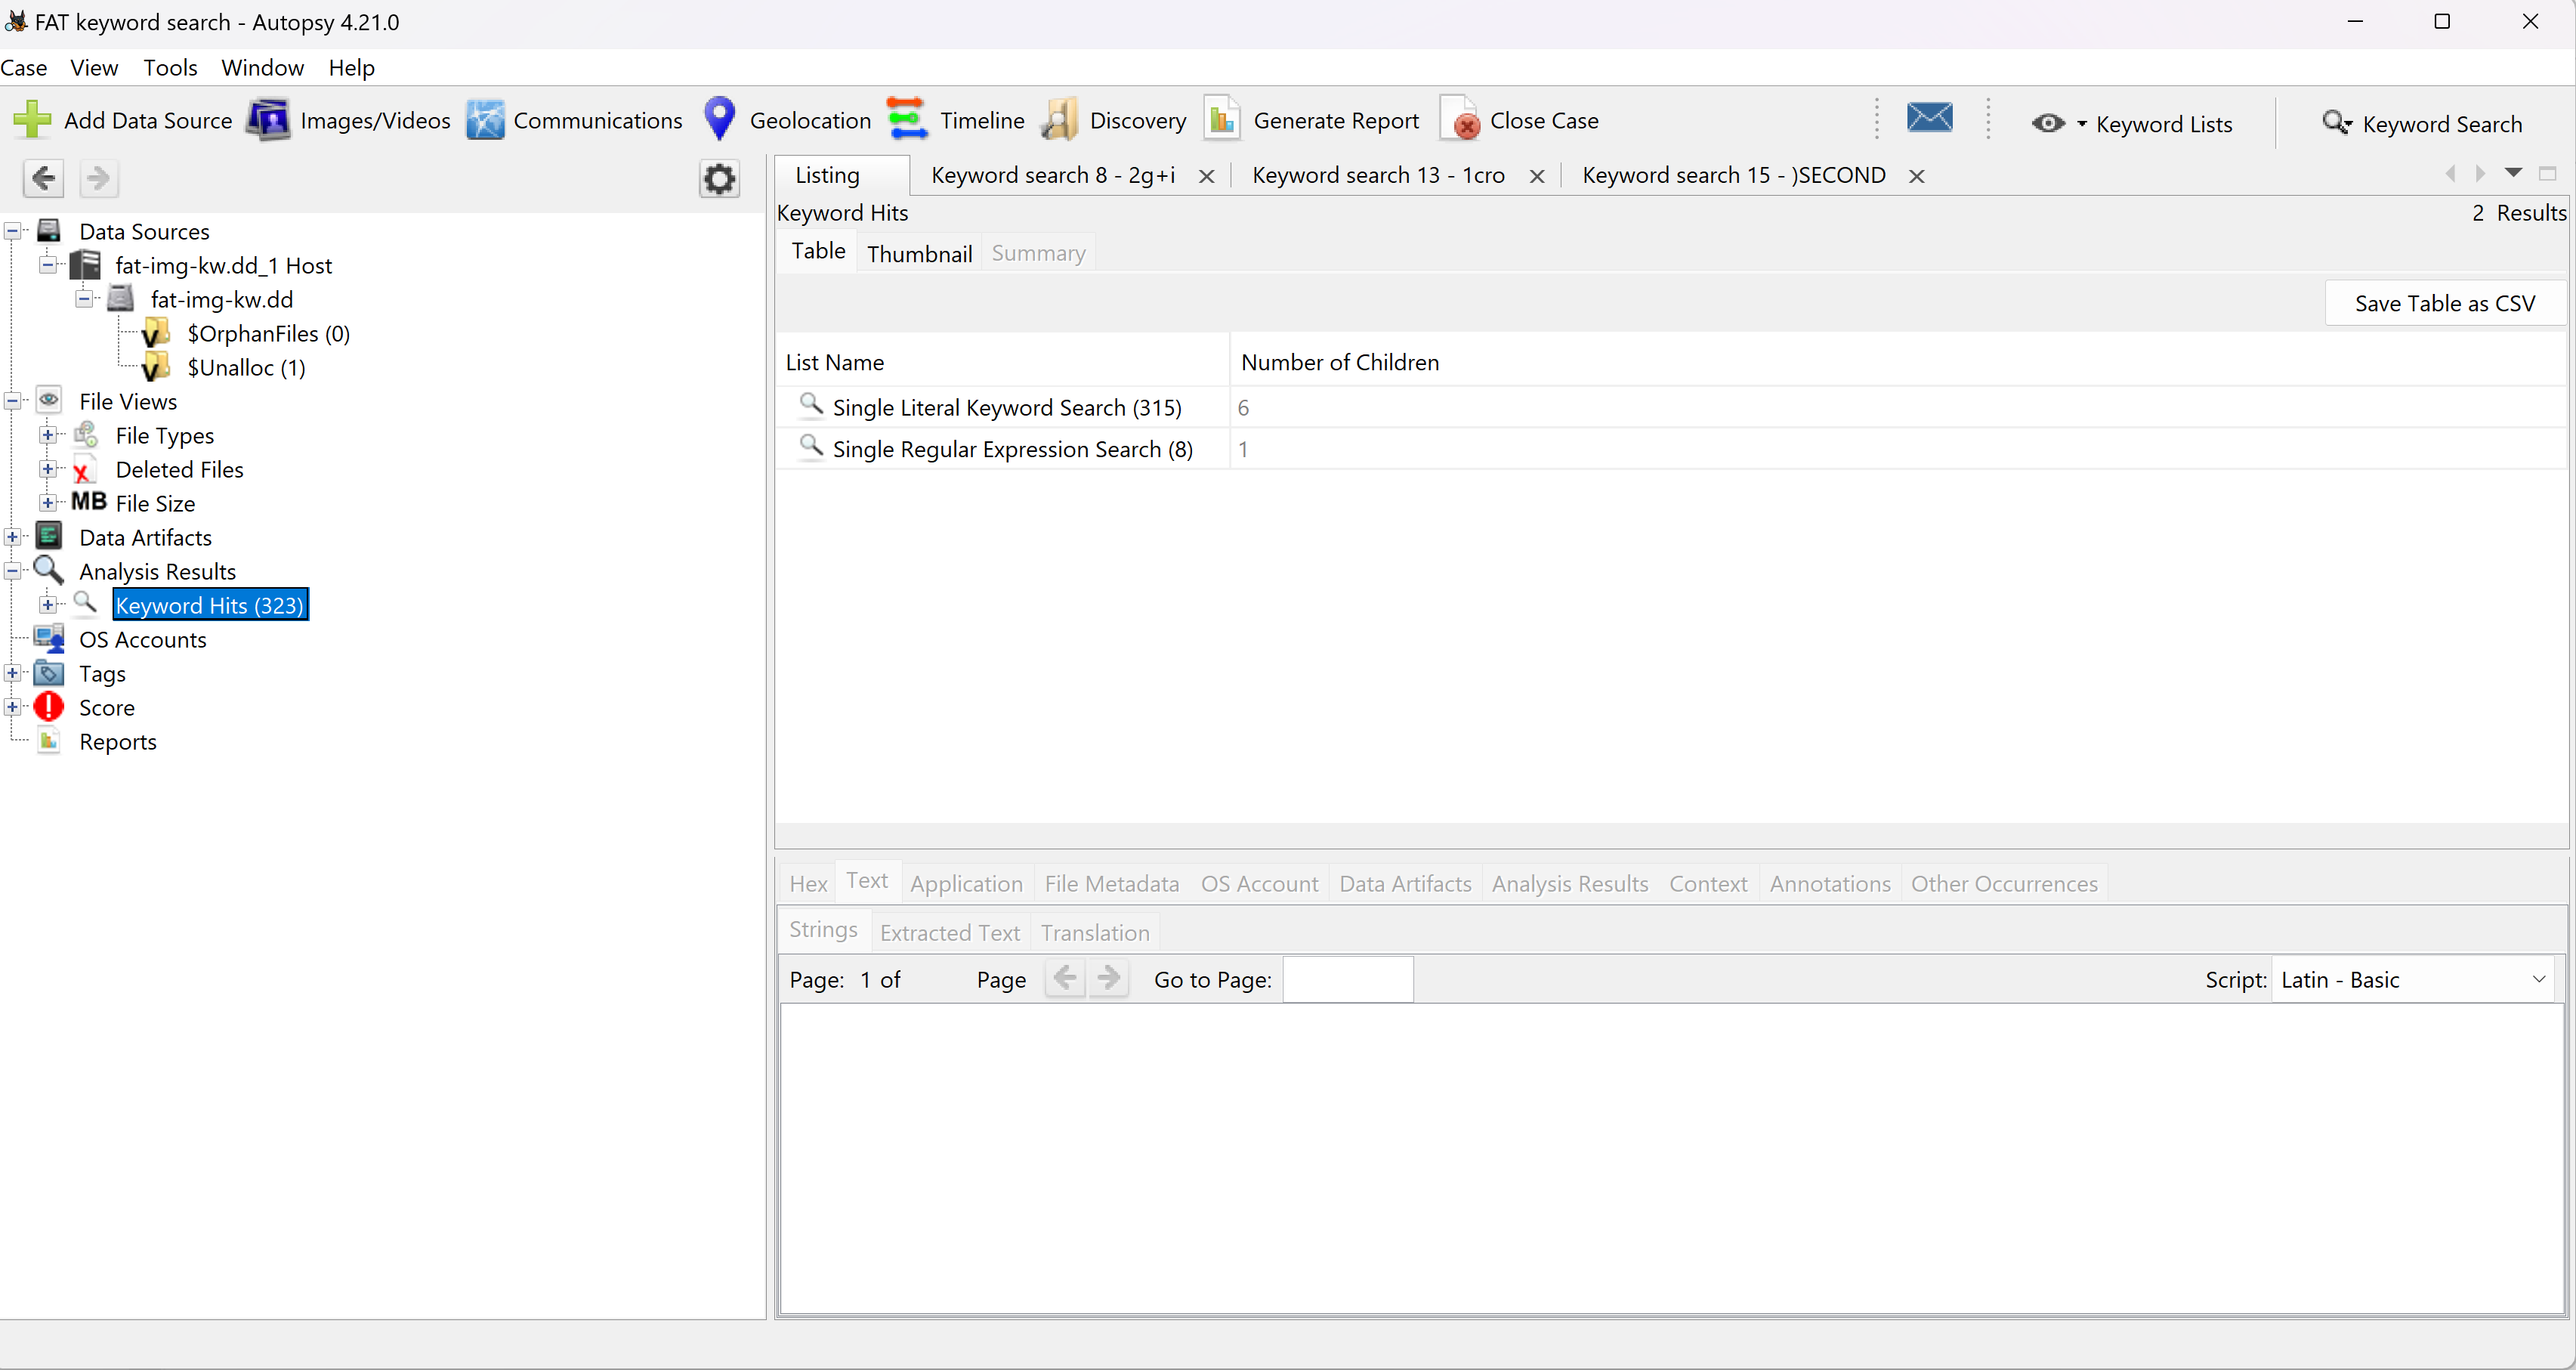
\includegraphics[width=0.75\textwidth]{6/6.2/Search Results for keyword.png}
\end{center}

\begin{center}
    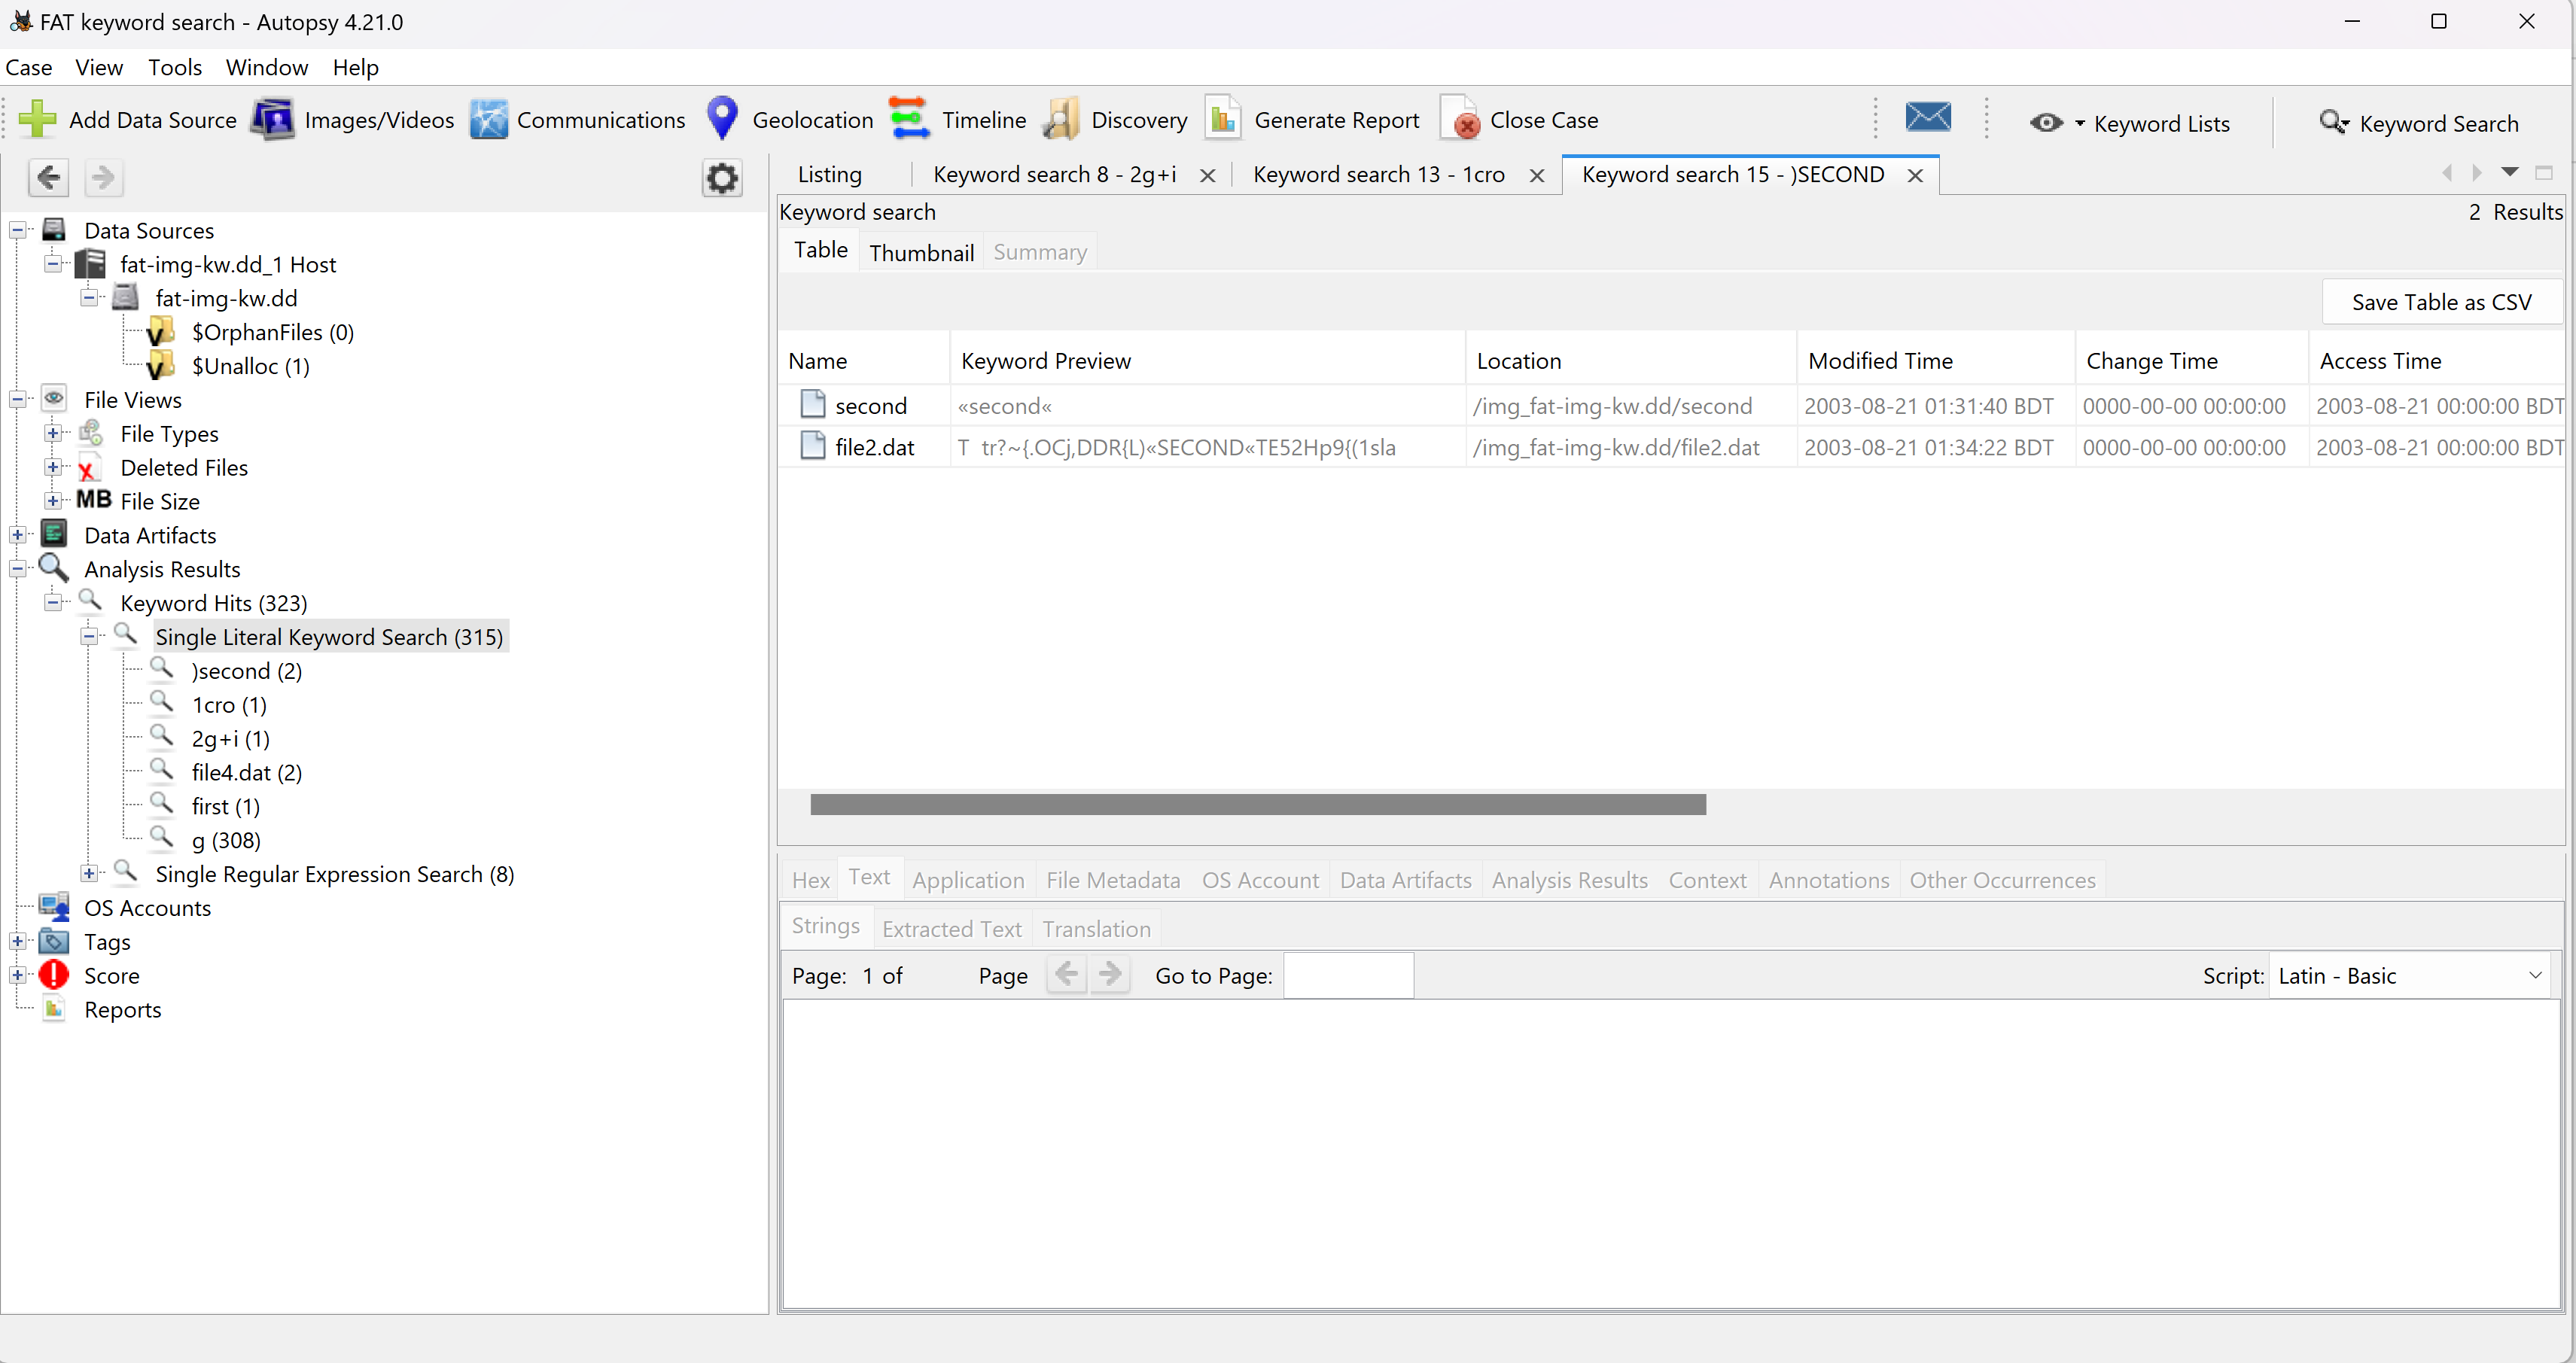
\includegraphics[width=0.75\textwidth]{6/6.2/Search Results for keyword _second_.png} \\
    The MD5 of the image is bac12239bd466fa6c86ceb0b0426da0a.
\end{center}

\subsubsection*{Conclusion}
In Autopsy, users have the capability to search for keywords within the data source. The search operation extends to file names, file content, and file metadata, including unallocated space within the data source. In this particular test, we conducted a keyword search within a FAT file system disk image. It's noteworthy that Autopsy, being a robust forensic tool, offers similar functionalities across a range of file systems such as NTFS, EXT3FS, and others.

\subsection{FTS Undelete Test}
\subsubsection*{Introduction}
The test image comprises a 6MB FAT file system containing six deleted files and two deleted directories. These files vary in size, from single cluster files to multiple fragments. It's important to note that no data structures were altered during this process to impede recovery efforts. The files were initially created and deleted in Windows XP and subsequently imaged in a Linux environment.

\subsubsection*{Source}
The disk image can be downloaded from here: \href{http://prdownloads.sourceforge.net/dftt/6-undel-fat.zip?download}{Disk Image Download Link} \\
The MD5 of the image is 4aeb06ecd361777242ab78735d51ace6.

\subsubsection*{Outputs from Autopsy}
\begin{center}
    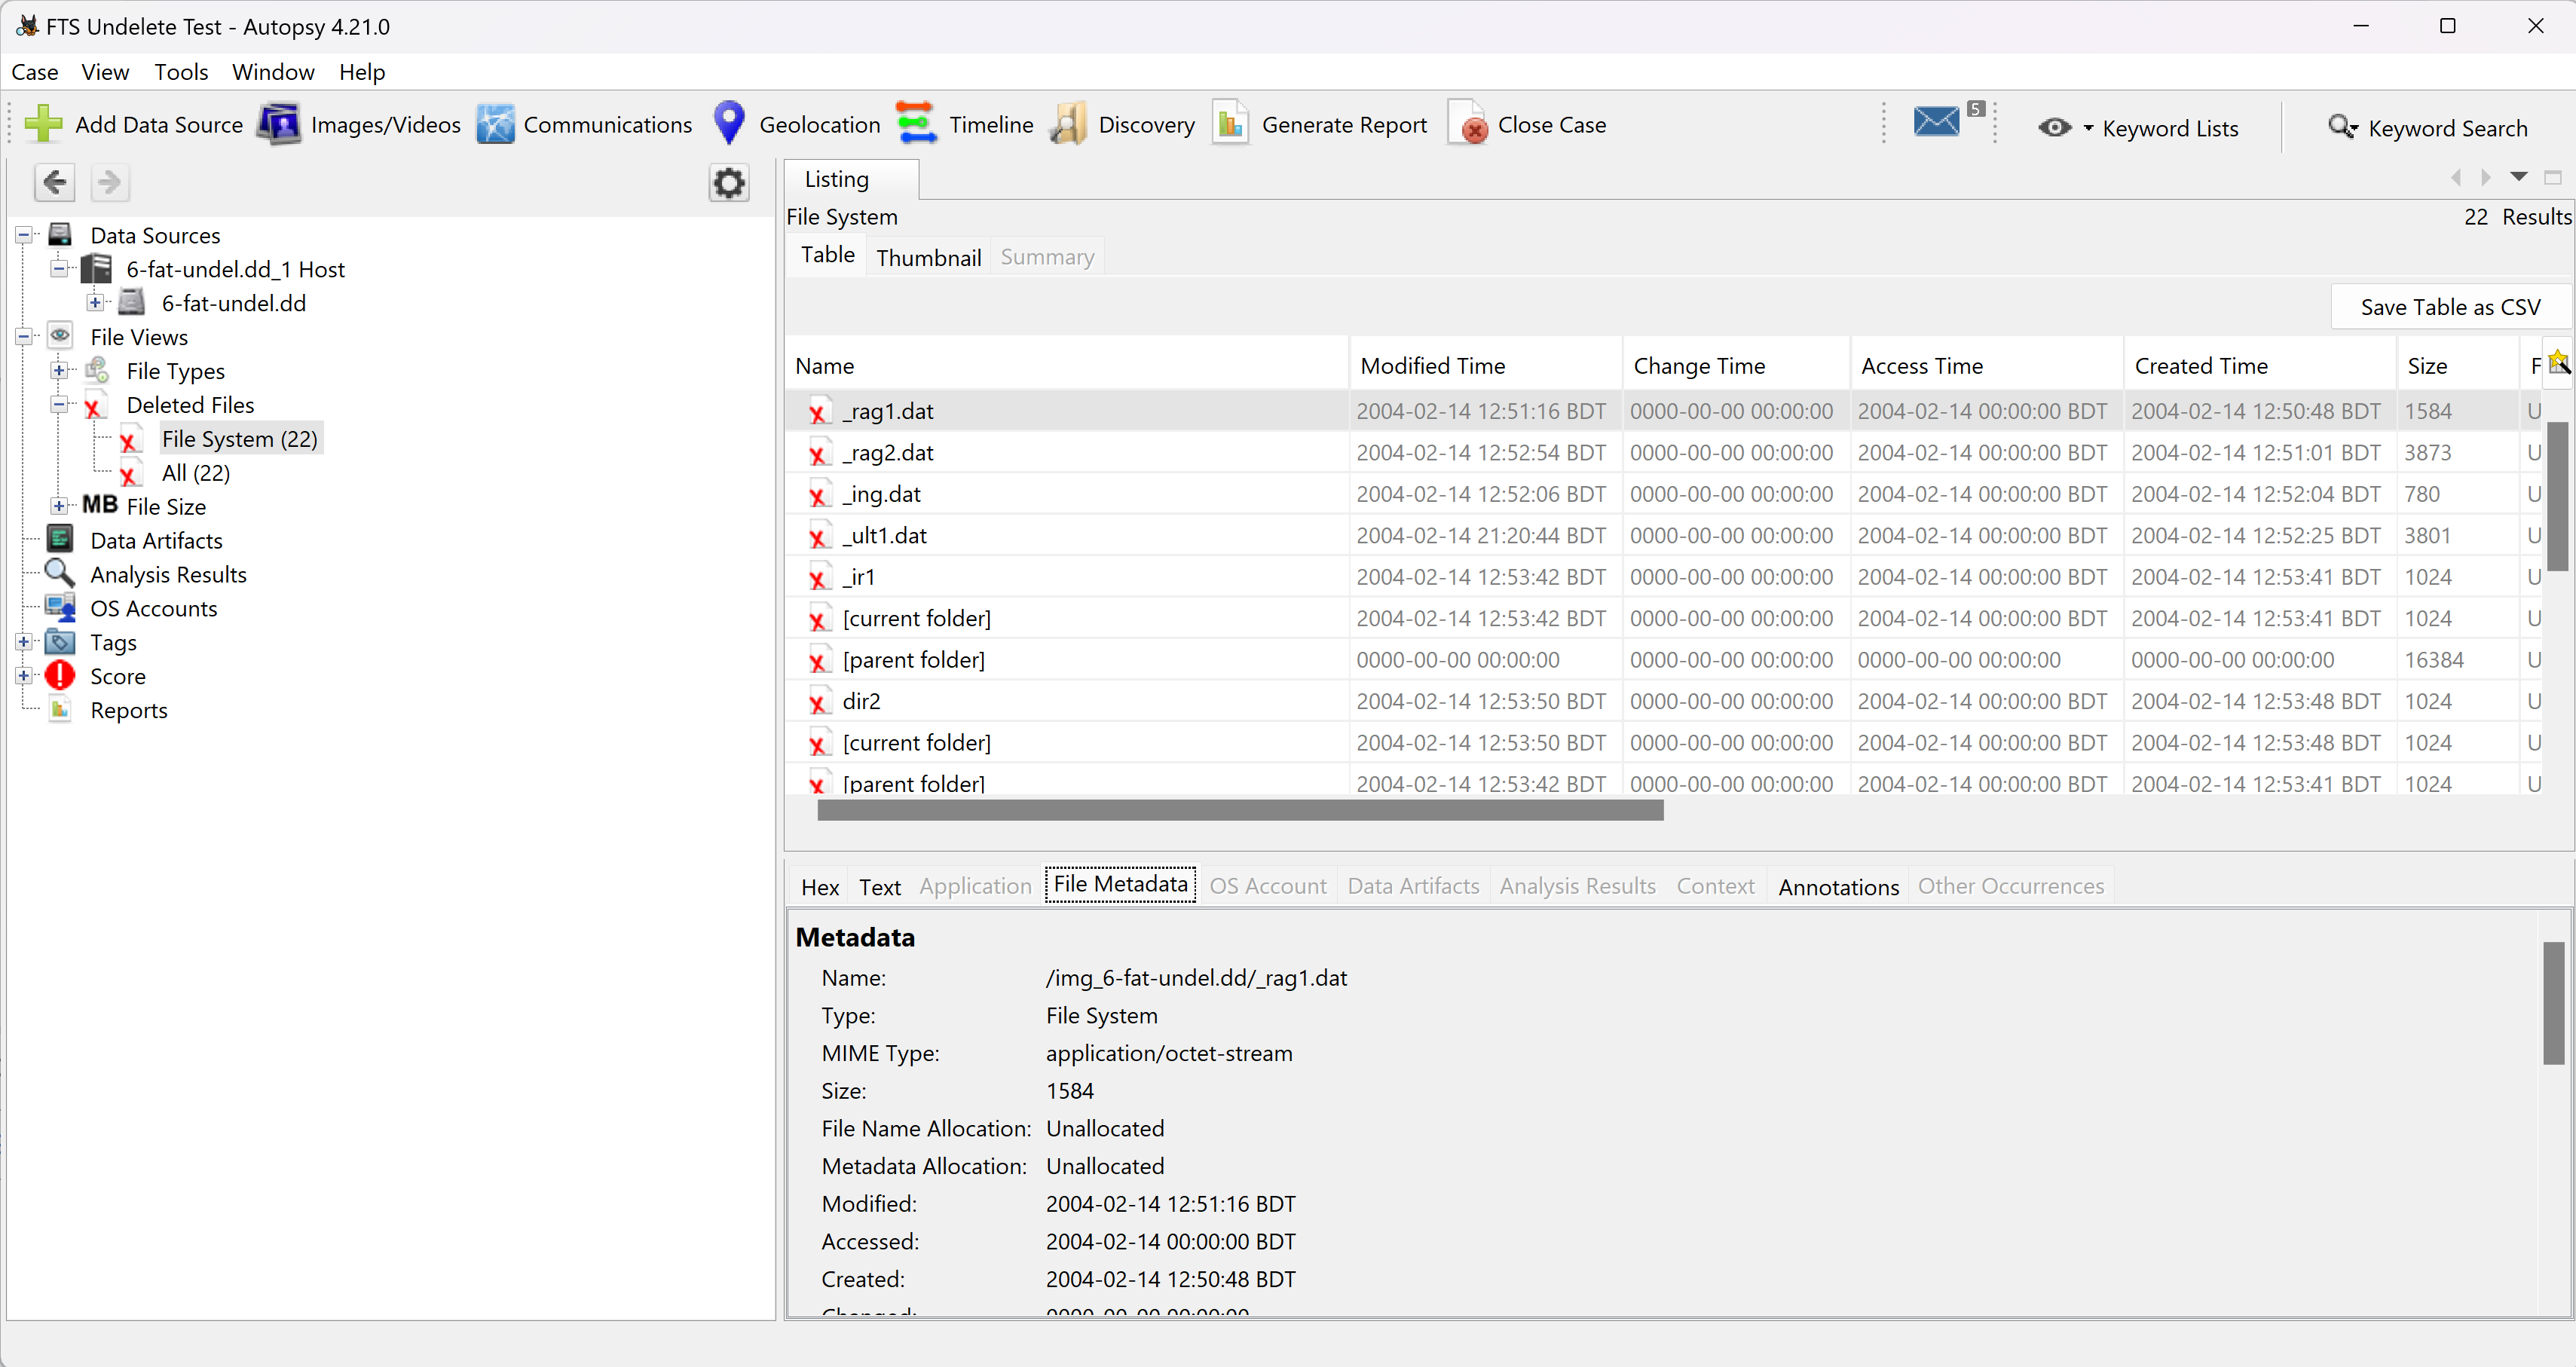
\includegraphics[width=0.75\textwidth]{6/6.3/FTS Deleted Files.png}
\end{center}

\subsubsection*{Conclusion}
Autopsy is capable of recovering and presenting deleted files and directories found within a file system.

\subsection{JPEG Search Test}
\subsubsection*{Introduction}
The provided test image represents an NTFS file system housing a collection of 10 JPEG images. Among these images are files with misleading extensions, JPEGs embedded within ZIP and Word files, as well as those stored in alternate data streams. The primary aim of utilizing this test image is to evaluate the effectiveness of automated tools designed for locating JPEG images.
\subsubsection*{Source}
The disk image can be downloaded from here: \href{http://prdownloads.sourceforge.net/dftt/8-jpeg-search.zip?download}{Disk Image Download Link} \\
The MD5 of the image is 9bdb9c76b80e90d155806a1fc7846db5.

\subsubsection*{Outputs from Autopsy}
\begin{center}
    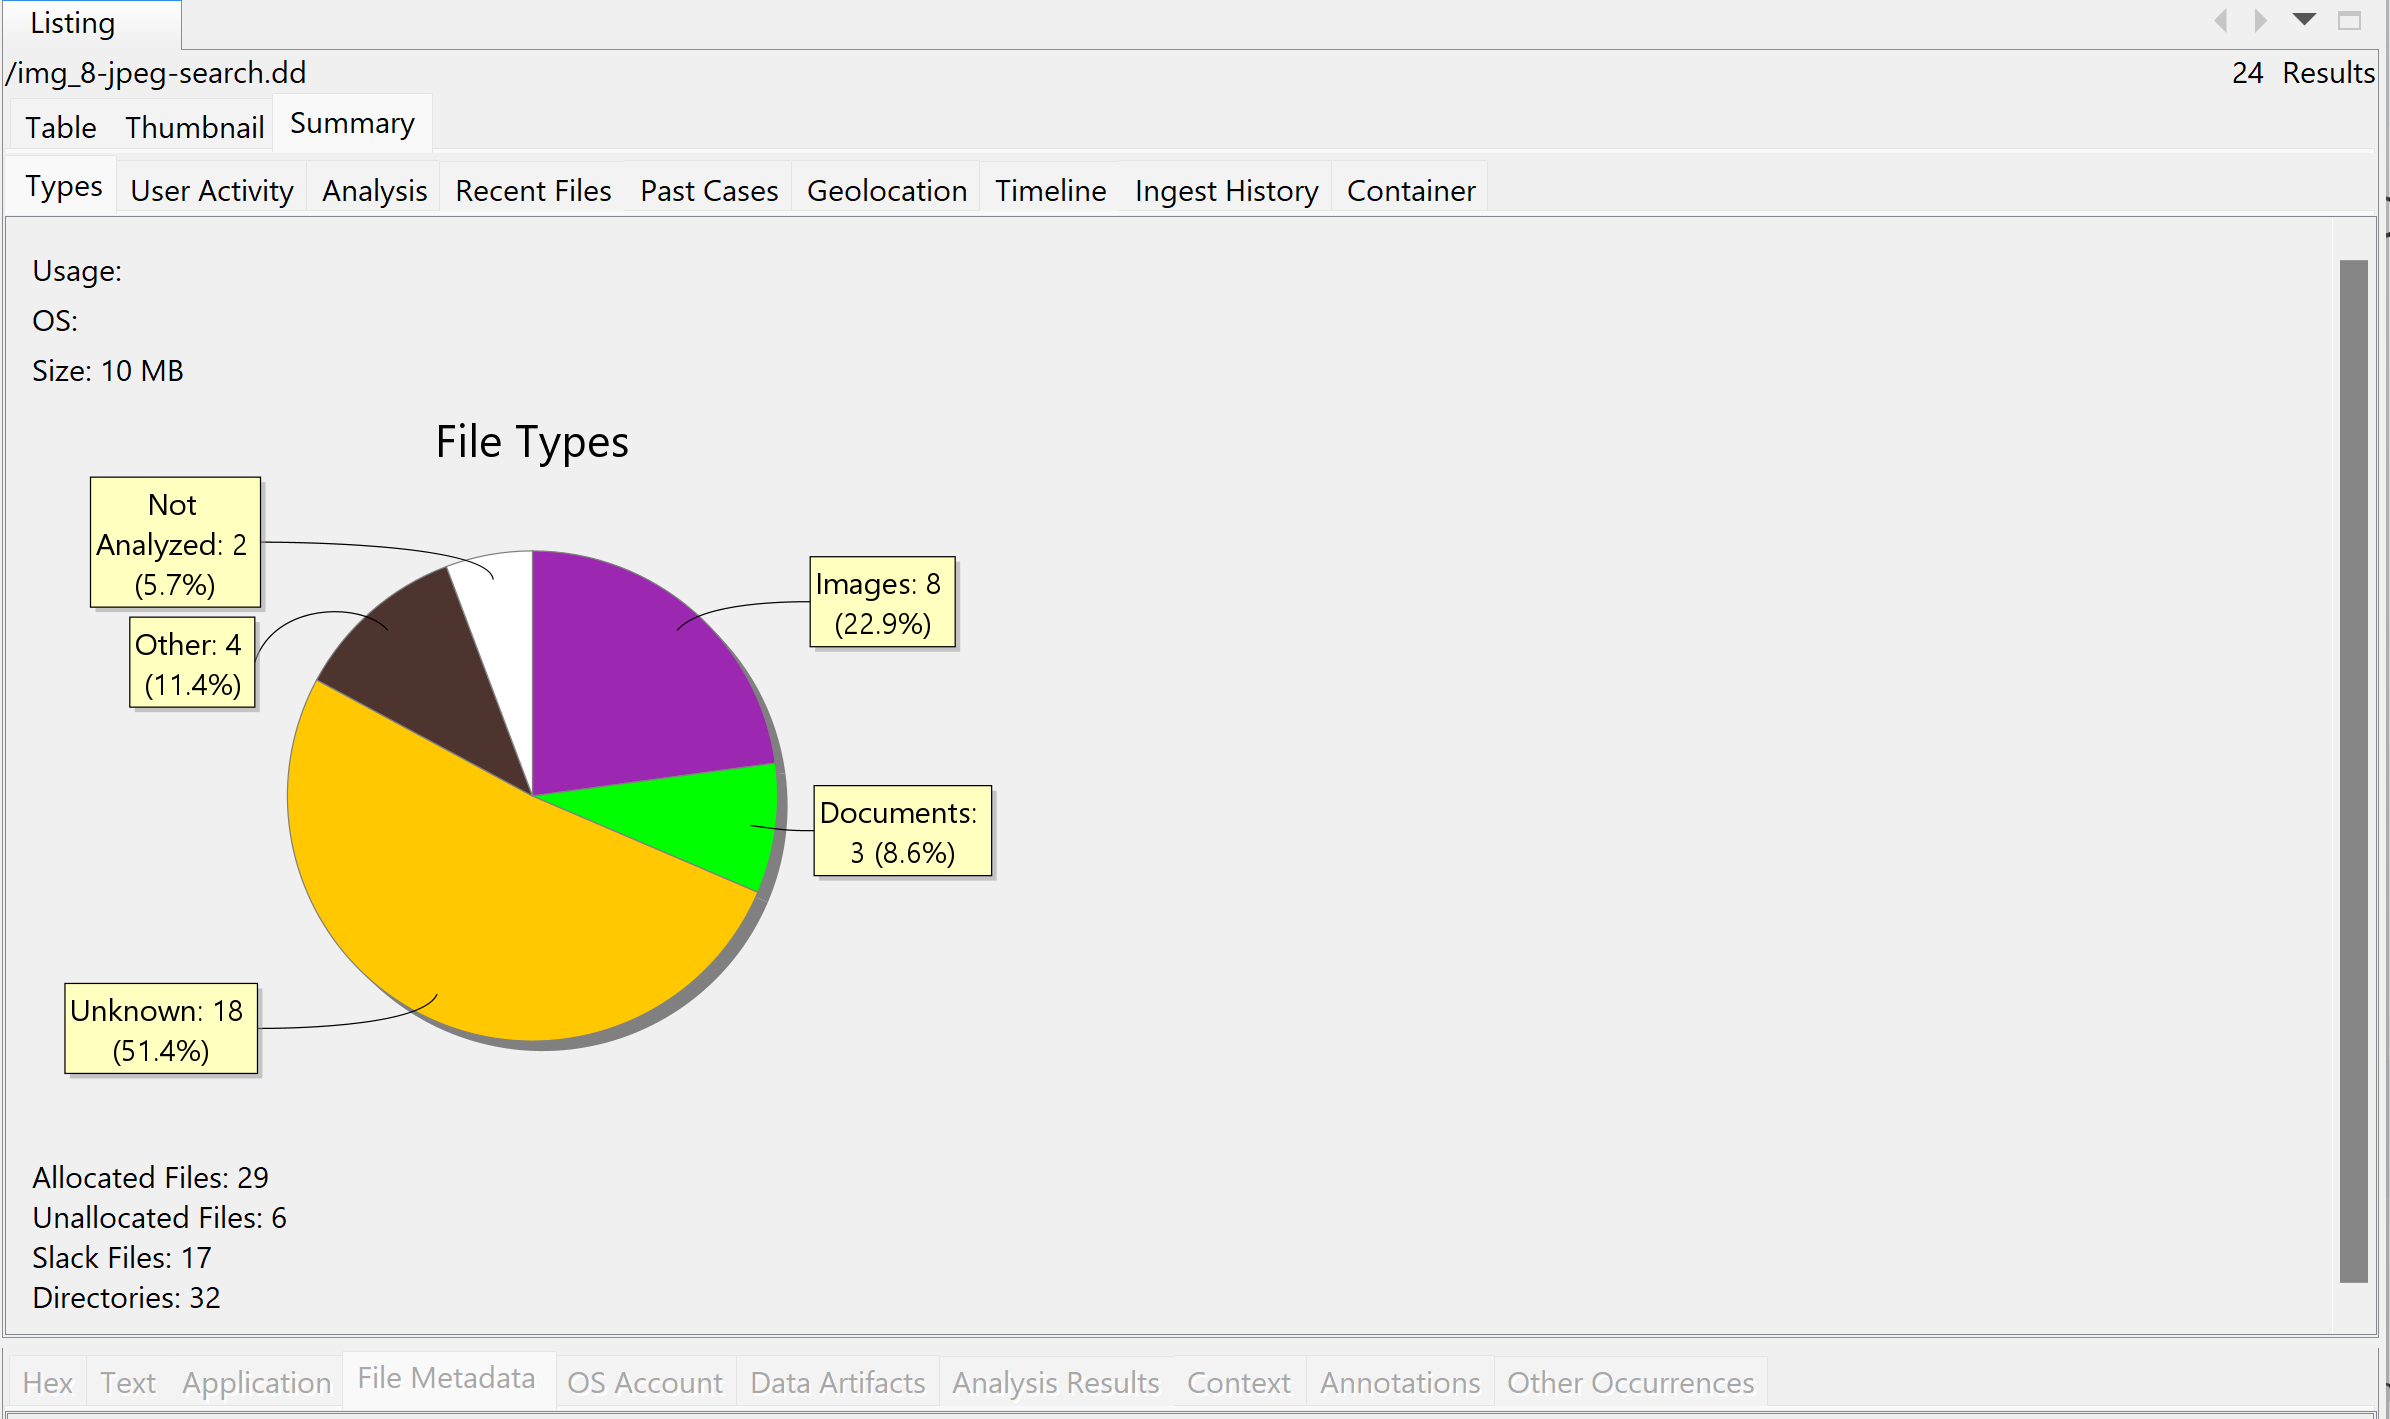
\includegraphics[width=0.75\textwidth]{6/6.4/Autopsy JPEG Search Summary.png}
\end{center}
As depicted in the figure below, Autopsy demonstrates its ability to identify JPEG images within the data source, even when the file extension is inaccurate. Furthermore, in cases where a file is labeled with a JPEG extension but does not contain JPEG image data, Autopsy accurately detects the correct file type and displays it accordingly.

\begin{center}
    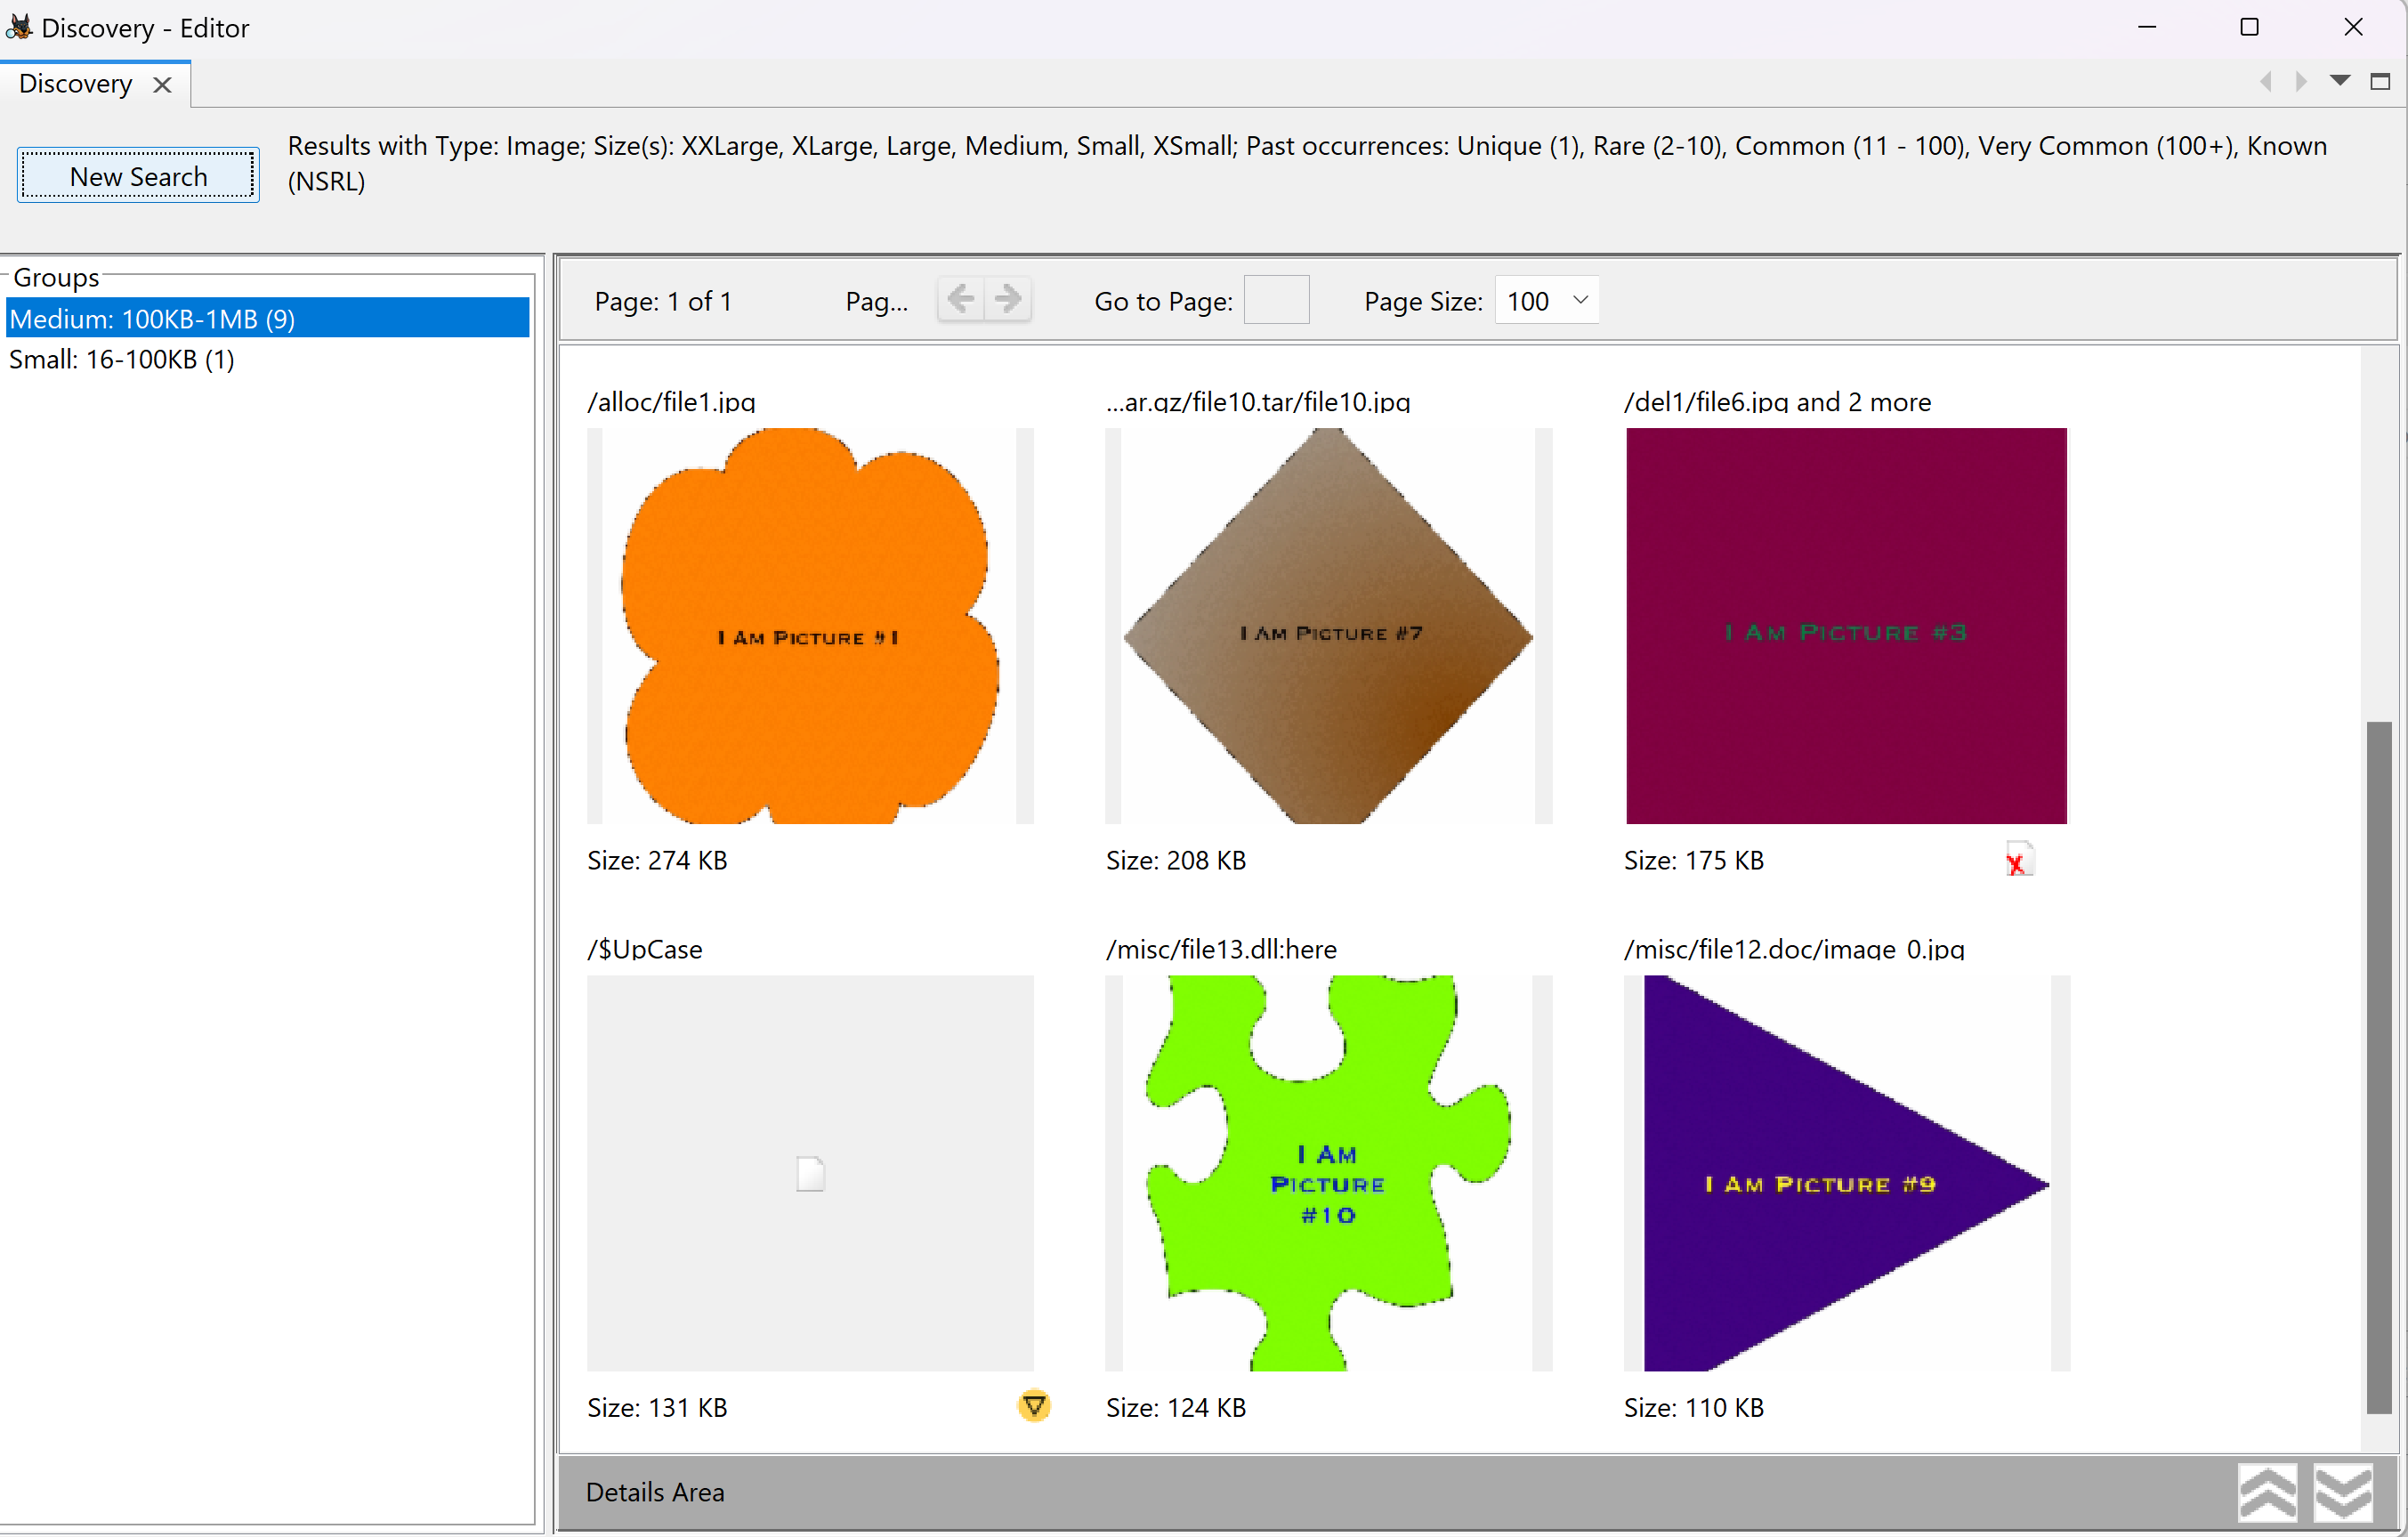
\includegraphics[width=0.75\textwidth]{6/6.4/All JPEG Images Found by Autopsy.png}
\end{center}

\begin{center}
    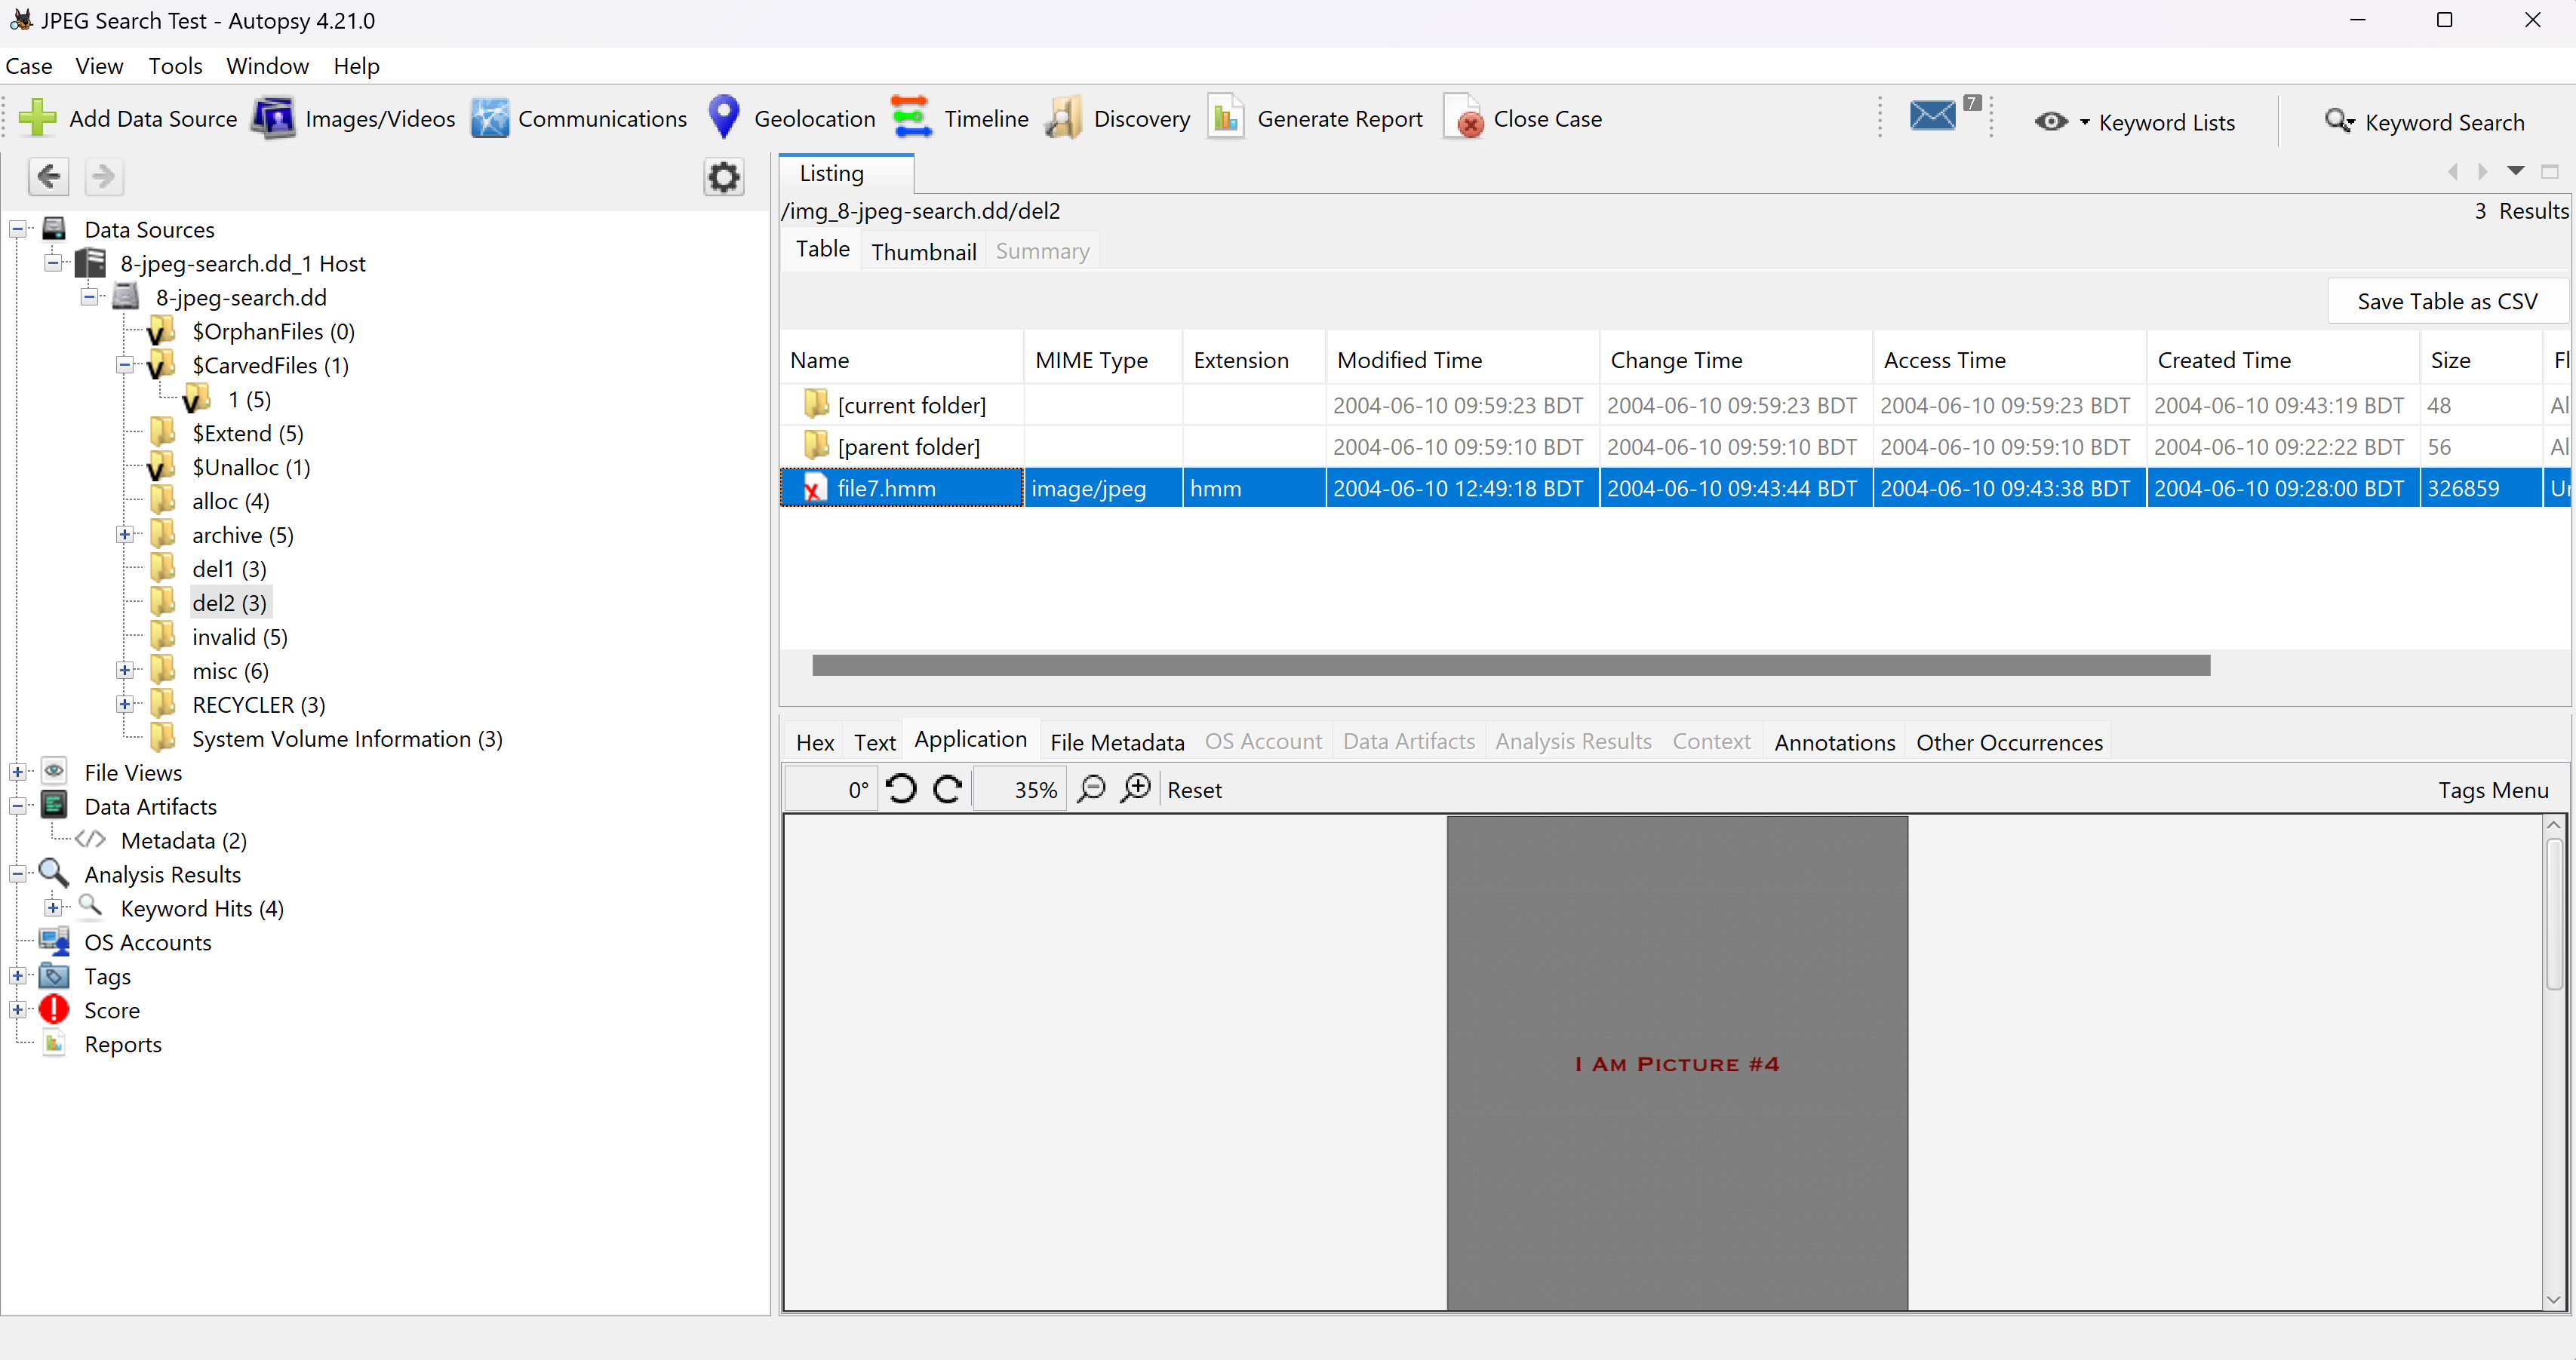
\includegraphics[width=0.75\textwidth]{6/6.4/Detecting Images with Corrupted Extension.png}
\end{center}

\begin{center}
    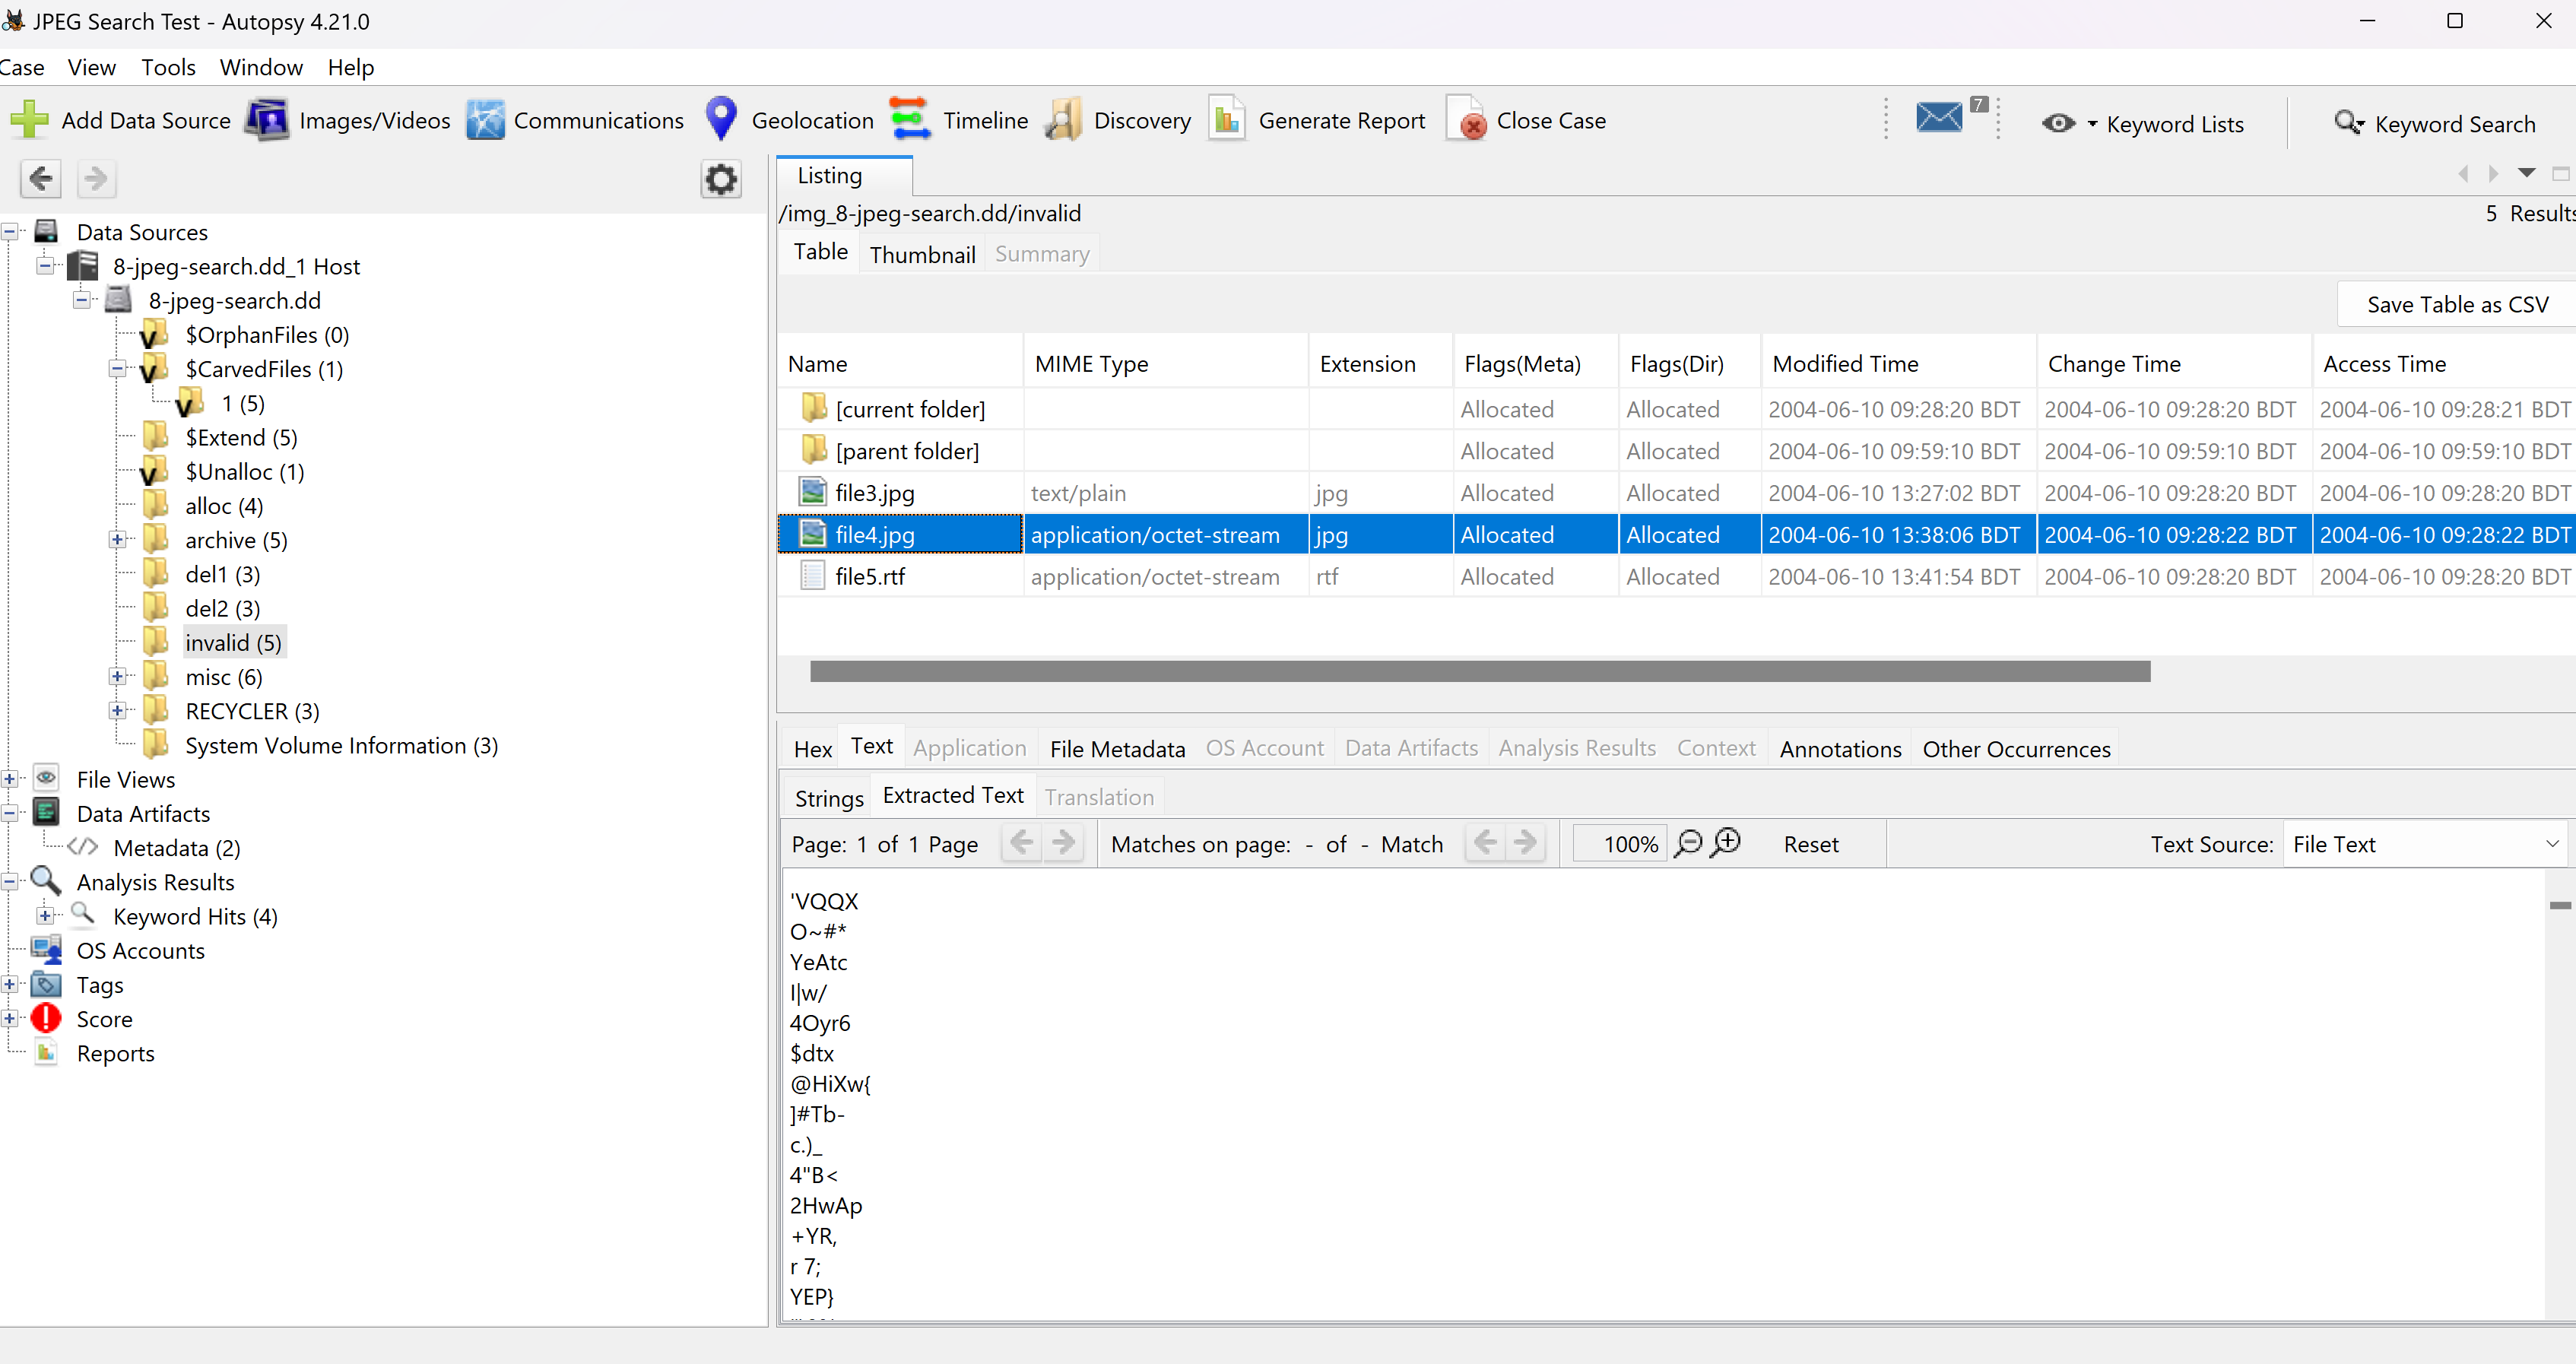
\includegraphics[width=0.75\textwidth]{6/6.4/Detecting Other File Types with JPEG Extension.png}
\end{center}

\subsubsection*{Conclusion}
Autopsy excels in identifying JPEG files, whether they have standard or non-standard extensions. It adeptly distinguishes false positives, even when files claim to be JPEGs but lack actual JPEG content. Autopsy can handle partial JPEGs, accurately recognizing valid signatures even without complete headers and footers. It effectively recovers deleted JPEGs, regardless of their extensions, and deals proficiently with deleted JPEGs with incorrect extensions. Autopsy's capabilities extend to locating and extracting embedded JPEGs within archive formats and unconventional file structures. It also excels in recognizing and extracting JPEGs embedded within document files and detecting hidden JPEGs within alternate data streams, making it a valuable tool for forensic analysis.

\subsection{NTFS Autodetect Test}
\subsubsection*{Introduction}
This test includes four images. One image is a disk image comprising two partitions, with each partition also provided as an individual file. The fourth image is an additional partition image. The objective of this test case is to evaluate the file system detection capabilities of analysis tools. While a typical partition usually contains only one file system, certain file system layouts allow for multiple file systems within a single partition. In this scenario, each partition within the disk image contains two file systems. Specifically, the first partition is formatted for NTFS and Ext2, the second for NTFS and UFS2, and the third for NTFS and UFS1. Both file systems are legitimate and can be mounted within their respective operating systems. The test aims to determine whether a tool will correctly identify the presence of two valid file systems or if it will only display one while concealing the other.
\subsubsection*{Source}
The disk image can be downloaded from here:
\href{http://prdownloads.sourceforge.net/dftt/10b-ntfs-autodetect.zip?download}{Disk Image Download Link} \\
This test case has one ’raw’ disk image and two ’raw’ partition images. In total, the images are 275 MB, but they compress to under 1 MB.\\
The MD5 of the disk image is 9225ff95b92311a28b2224e9dc324231,\\
Partition 1 is 6bd741152ccedd50e12623af5eeba803,\\
Partition 2 is 0b768efb1011b047c9831c1e00d1706c,\\ Partition 3 is 5984253cad72d4950c15a9e679139daf

\subsubsection*{Image Details}

The disk image \texttt{10-ntfs-disk.dd} contains a DOS partition table with two partitions: \texttt{10-ntfs-part1.dd} and \texttt{10-ntfs-part2.dd}. Both partitions have a type of 0x07, indicating NTFS file systems. Let's explore the contents of each partition:

\begin{itemize}
    \item \texttt{10-ntfs-part1.dd}: Originating from the first partition within \texttt{10-ntfs-disk.dd}, this image was initially formatted as NTFS using Windows XP, housing the \texttt{ntfs.txt} file. Subsequently, the partition was formatted as Ext2, resulting in the creation of the \texttt{ext2.txt} file. Windows error-checking detected no issues with the NTFS file system.
    
    \item \texttt{10-ntfs-part2.dd}: Derived from the second partition of \texttt{10-ntfs-disk.dd}, this image was initially formatted as NTFS within Windows XP, containing the \texttt{ntfs.txt} file. However, a subsequent formatting process converted it to UFS2, inadvertently creating the \texttt{ufs1.txt} file. Despite the misformatting, Windows error-checking detected no issues. Notably, this partition was intended to be UFS1 but was erroneously formatted as FreeBSD UFS2.
    
    \item Additionally, the image \texttt{10-ntfs-part3.dd} does not reside within \texttt{10-ntfs-disk.dd} but was created due to the incorrect formatting of \texttt{10-ntfs-part2.dd} as UFS2 instead of UFS1. Initially formatted as NTFS using Windows XP, this partition contains the \texttt{ntfs.txt} file. Subsequent formatting transformed it into UFS1, resulting in the creation of the \texttt{ufs1.txt} file. Once again, Windows error-checking reported no issues with the NTFS file system.
\end{itemize}

This series of events underscores the complexity and potential errors inherent in partition formatting, while also showcasing the resilience of NTFS file systems under scrutiny.

\subsubsection*{Outputs from Autopsy}

\begin{center}
    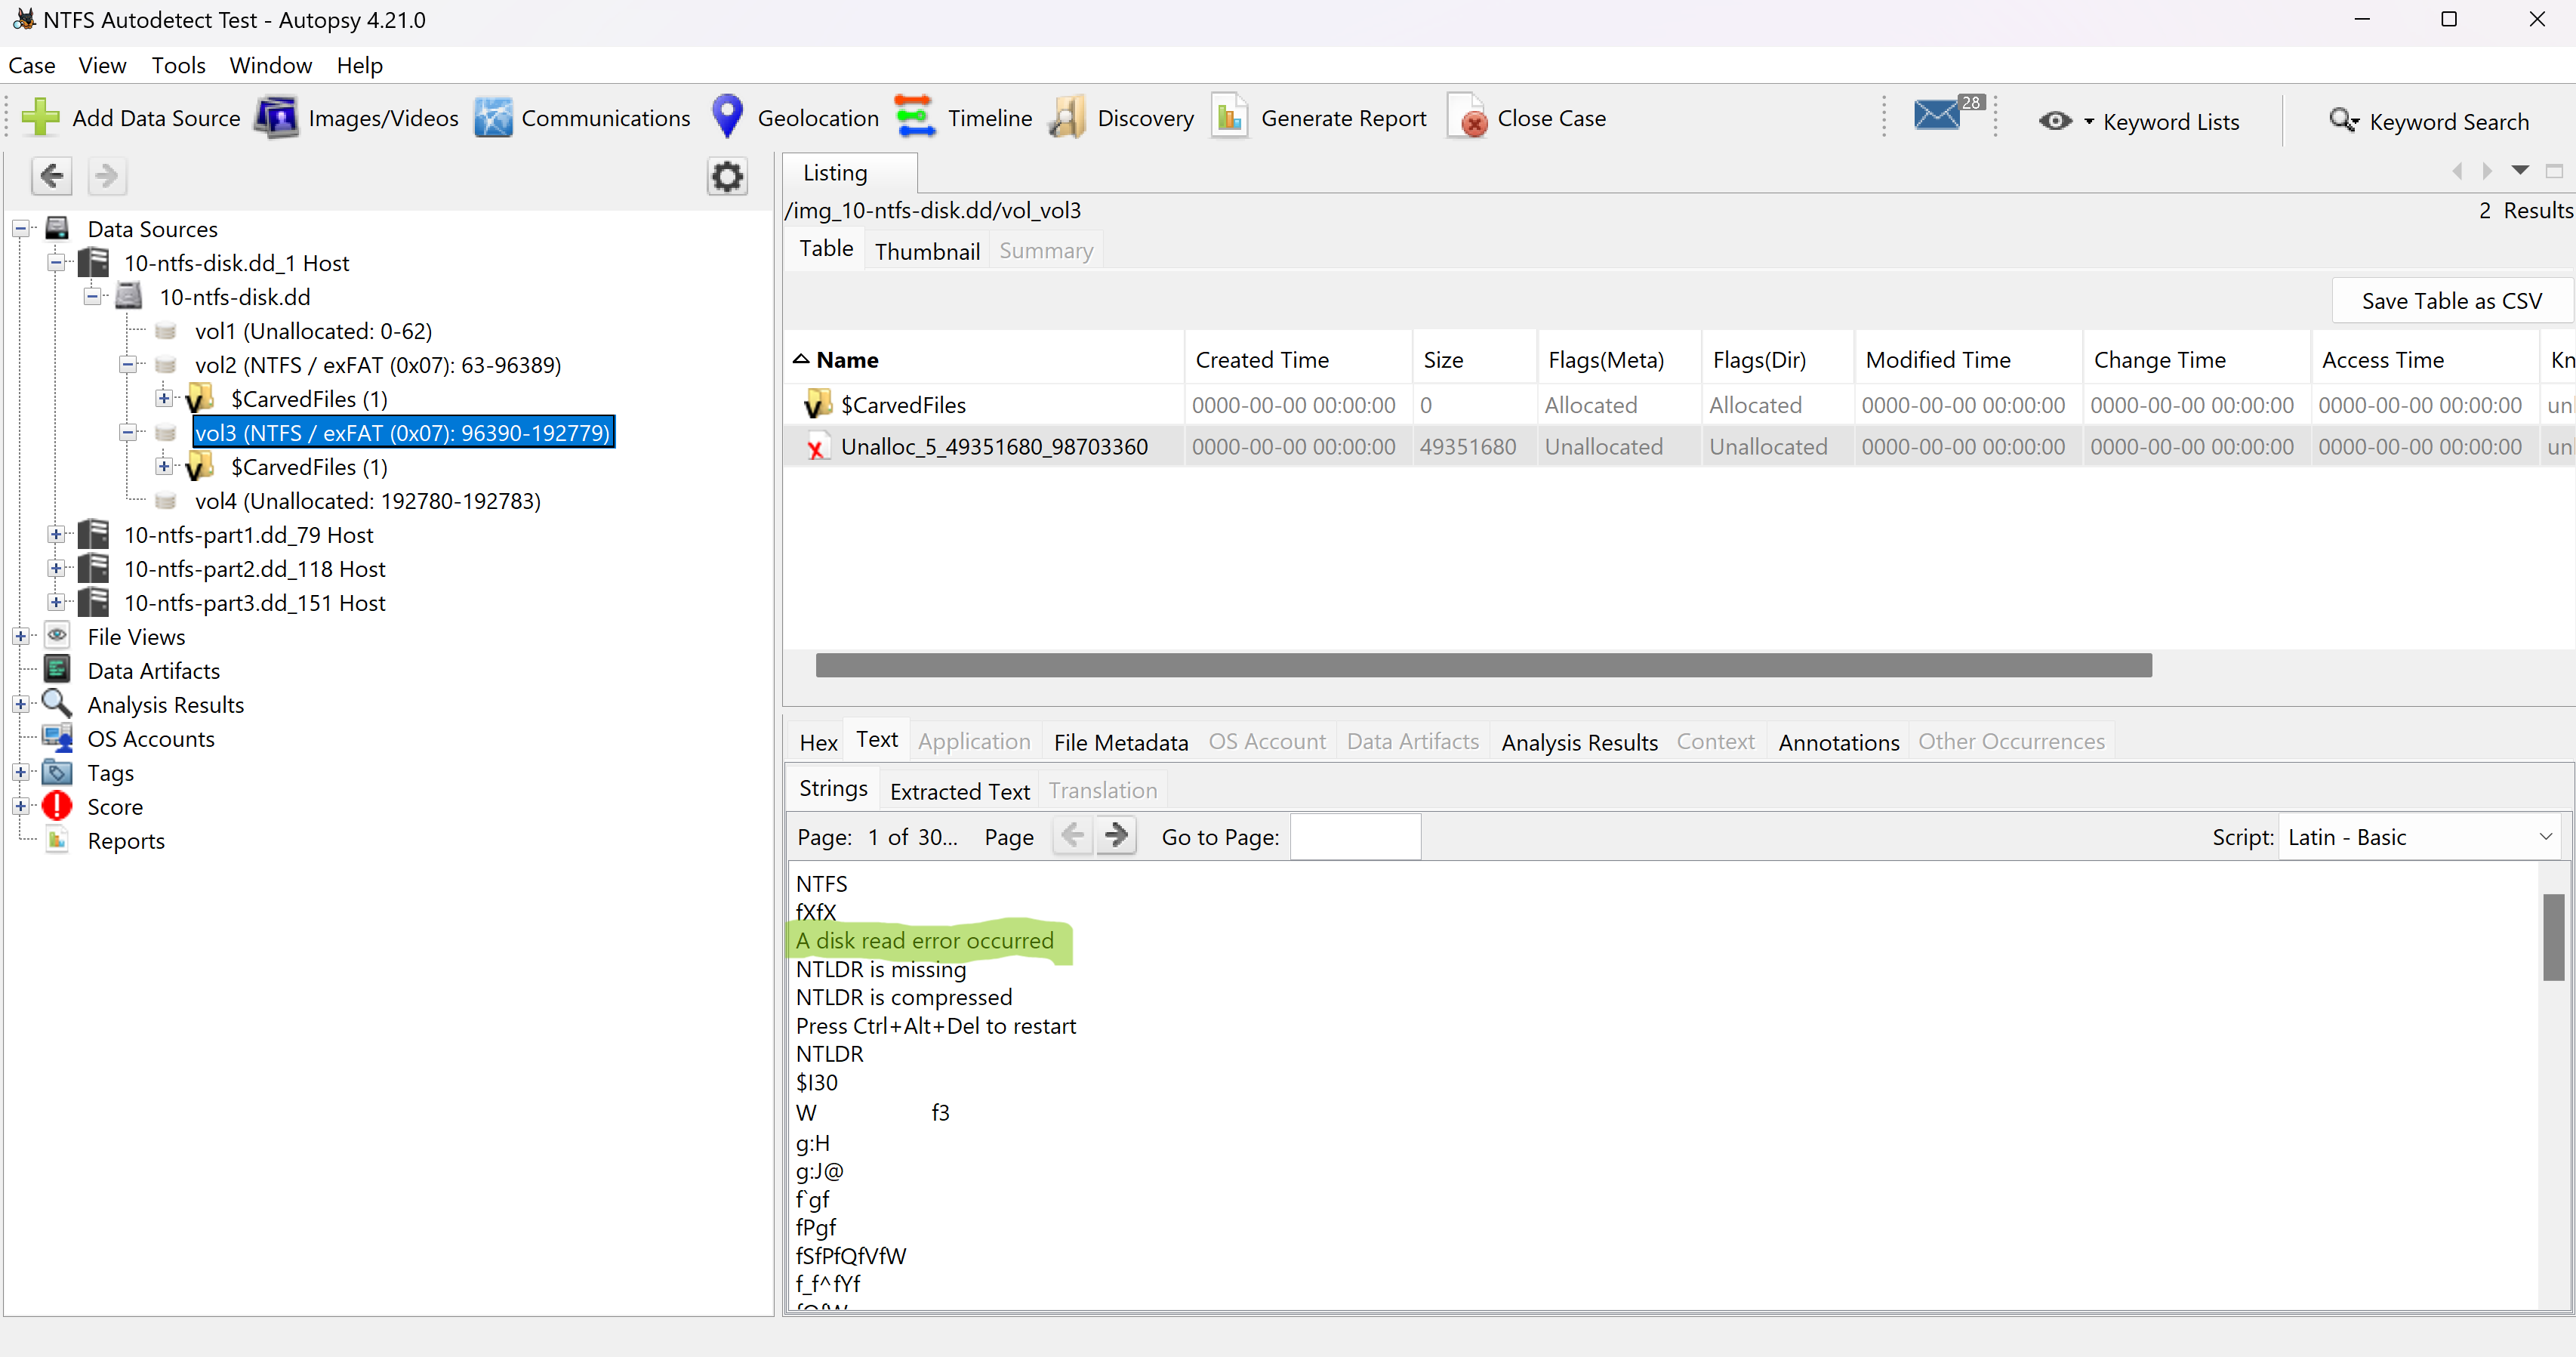
\includegraphics[width=0.4\textwidth]{6/6.5/Autopsy NTFS Autodetect-1.png}
\end{center}

\begin{center}
    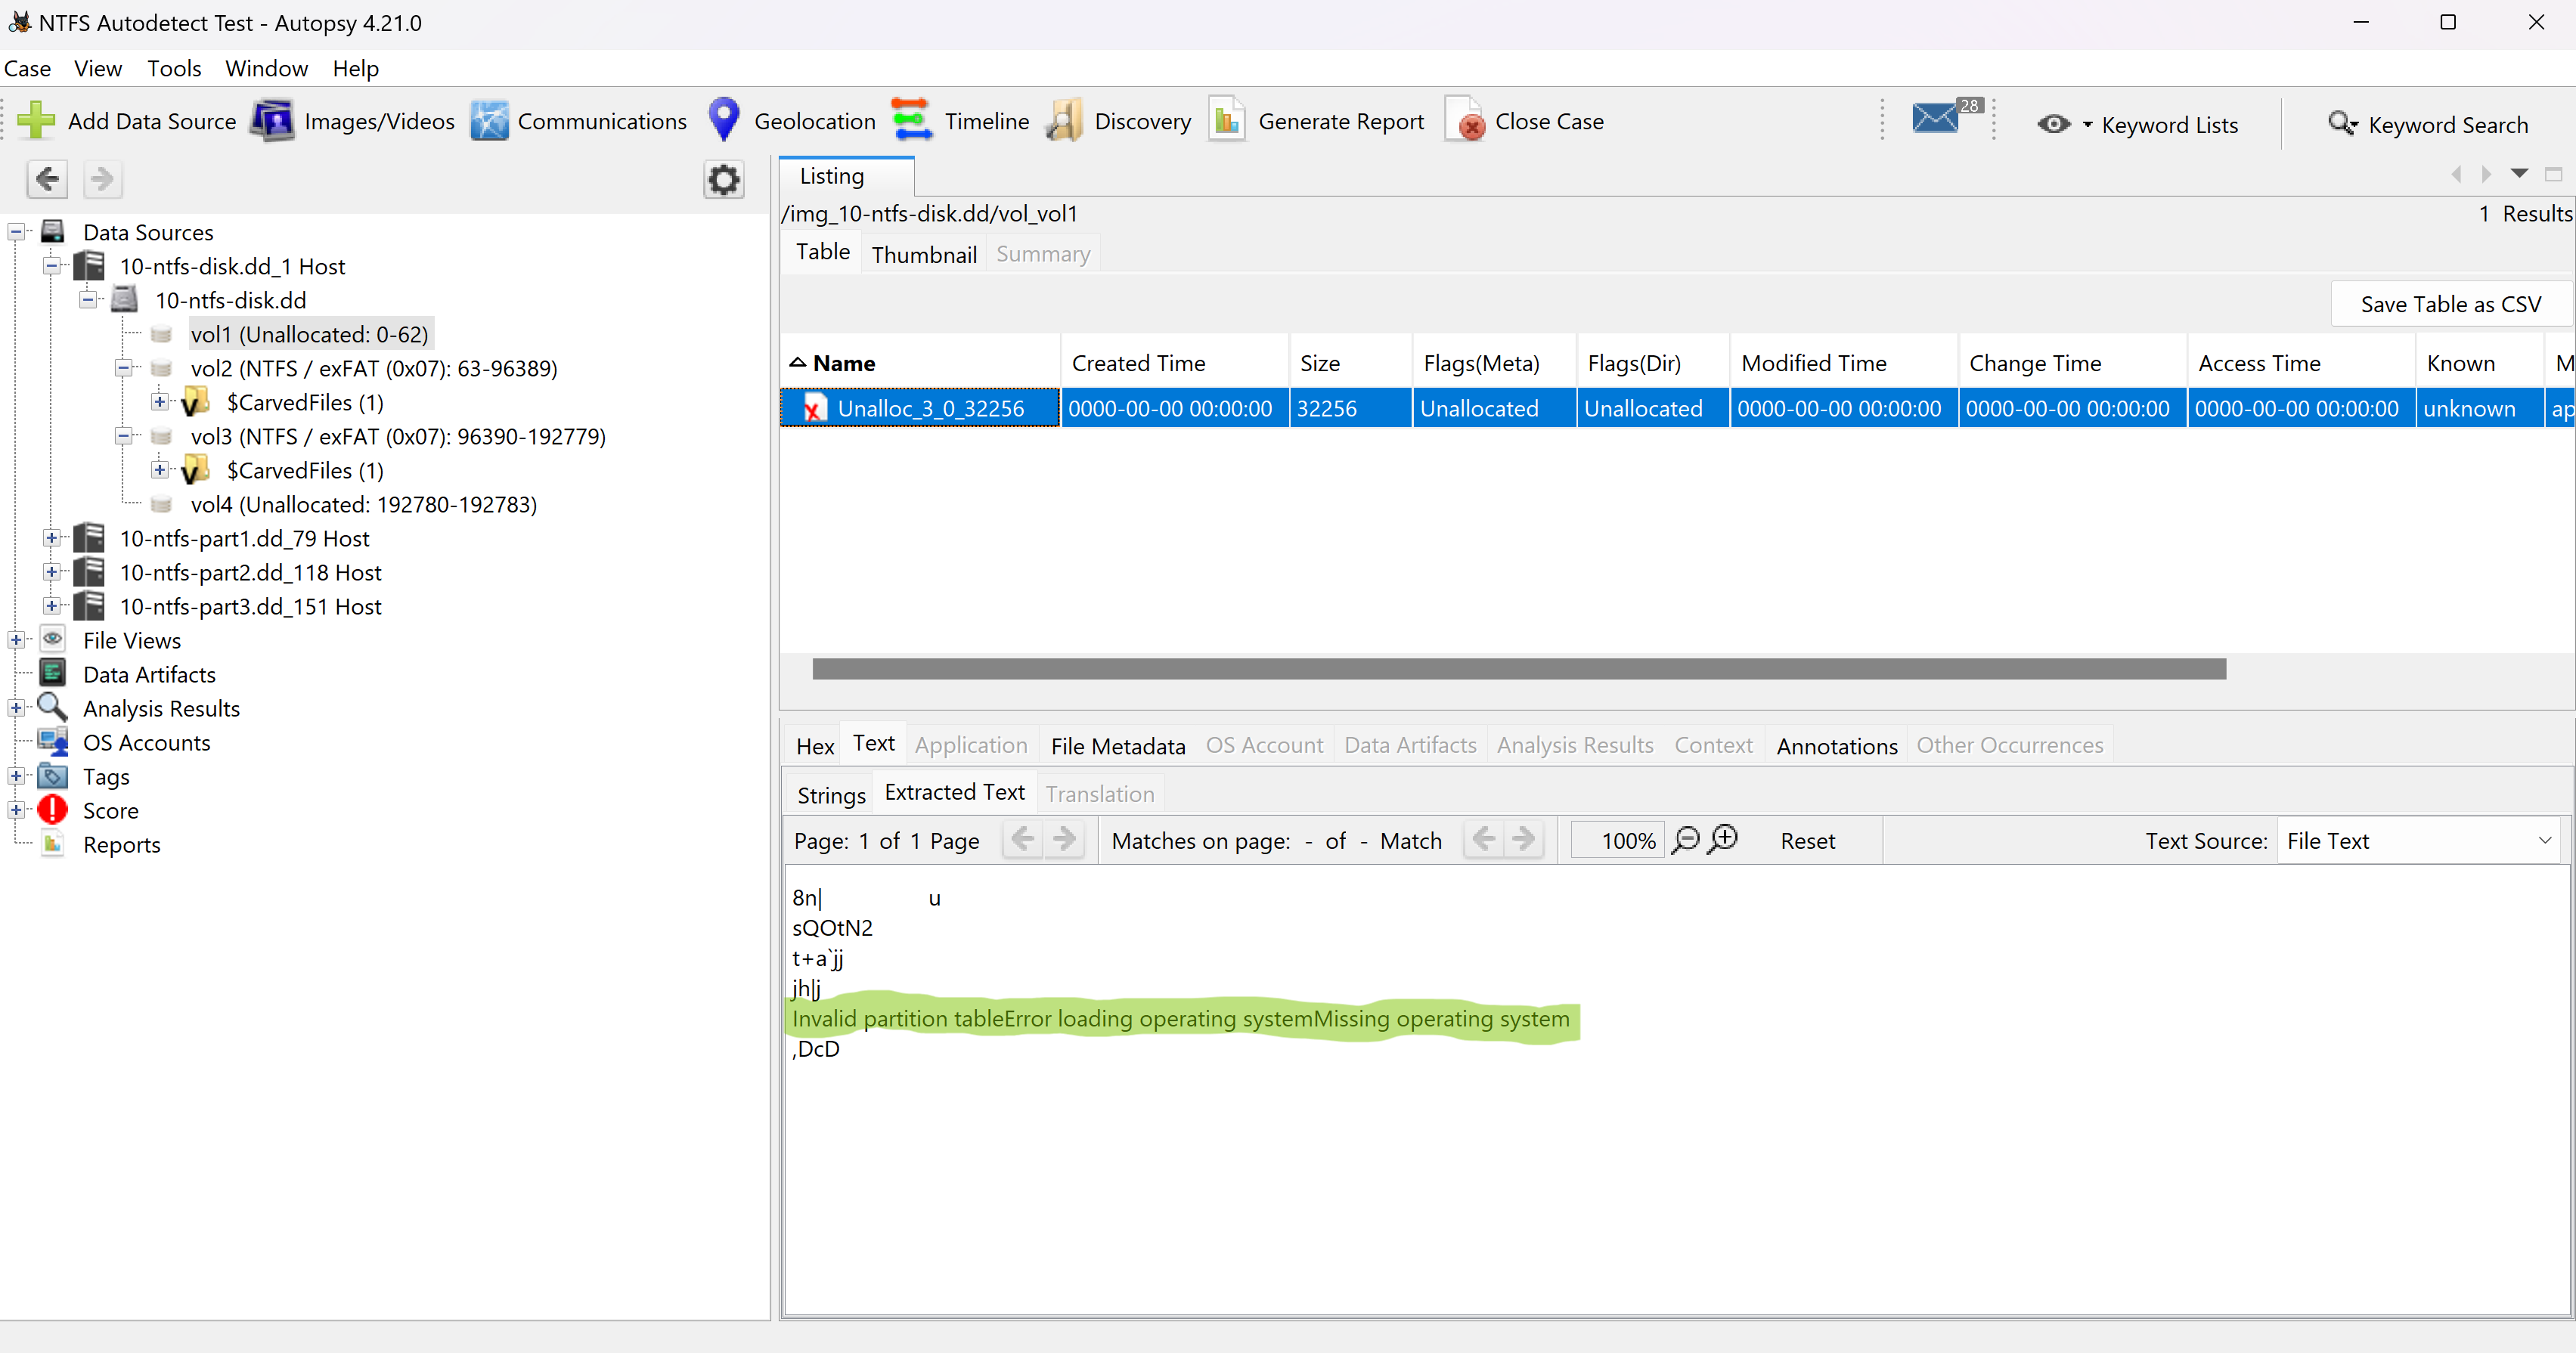
\includegraphics[width=0.4\textwidth]{6/6.5/Autopsy NTFS Autodetect-2.png}
\end{center}

\subsubsection*{Conclusion}
Autopsy can correctly detect and display multiple file systems within a partition.

\section{References}

To download Autopsy, visit: \href{https://www.autopsy.com/download/}{Autopsy Download Link} 

For more information about Autopsy, visit: \href{http://www.sleuthkit.org/autopsy/}{Autopsy Information Link} 

For digital forensics test images, visit: \href{https://dftt.sourceforge.net/}{Digital Forensics Test Images Link}
\end{document}

